\documentclass{article}[draft]
\usepackage[utf8]{inputenc}
\usepackage{amsmath}
\usepackage{amssymb}
\usepackage{color}
\usepackage{amsmath}
\newtheorem{theorem}{Theorem}[section]
\newtheorem{definition}{Definition}[section]
\newcommand{\R}{\mathbb{R}}
\newcommand{\norm}[1]{\left\lVert#1\right\rVert}


\newcommand{\myint}{\int\limits}
\newcommand{\diff}[1]{\, d#1}
\newcommand{\vect}[1]{\mathbf{#1}}
\usepackage{mleftright}
\newcommand{\of}[1]{\mleft( #1 \mright)}
\newcommand{\ddt}[1]{\partial_t #1}
\newcommand{\vth}{v_\textrm{th}}
\newcommand{\reals}{\mathbb{R}}
\newcommand{\RR}{\mathbb{R}}
\newcommand{\vr}{v}
%\newcommand{\vtheta}{\theta_{\vect{v}}}
%\newcommand{\vphi}{\varphi_{\vect{v}}}
%\newcommand{\vr}{v_{r}}
\newcommand{\vtheta}{v_{\theta}}
\newcommand{\vphi}{v_{\varphi}}
\newcommand{\vomega}{v_{\omega}}
\newcommand{\vrunit}{\hat{\vect{v}}_{r}}
\newcommand{\vthetaunit}{\hat{\vect{v}}_{\theta}}
\newcommand{\vphiunit}{\hat{\vect{v}}_{\varphi}}
\newcommand{\lp}[2]{L^{(#1)}_{#2}}
\newcommand{\lph}[2]{\tilde{L}^{(#1)}_{#2}}
\newcommand{\bfun}[2]{\Phi^{(#1)}_{#2}}
\newcommand{\tfun}[2]{\Psi^{(#1)}_{#2}}
\newcommand{\nfun}[2]{N^{(#1)}_{#2}}
\newcommand{\maxp}[2]{P^{(#1)}_{#2}}
\newcommand{\diffm}[3]{D^{(#1)}_{#2,#3}}
\usepackage{pgfplots}
\pgfplotsset{compat=newest}
\usepackage{float}
\usepackage{algorithm}
\usepackage{algpseudocode}

\title{Scalable deterministic numerical methods for the Boltzmann equation}
%\author{Milinda Fernando}
%\date{February 2014}

\begin{document}

%\begin{titlepage}
\maketitle
%\end{titlepage}

\section{Boltzmann Equation summary}
The Boltzmann equation is a nonlinear integro-differential equation that describes the evolution of the particle density function $f : \R^3 \times \R^3 \times \R \rightarrow \R^{+}_0$. Independent variables for the above density function denotes, time ($t$), position vector ($x$), and the velocity ($v$). For a fixed time $t$, $f(x,v,t)dx dv$ represent the number of particles for the phase space volume element $dxdv$. 

We can write the Boltzmann equation in the absence of external force field can be written as below. 
\begin{equation}
    \partial_t f + v\cdot \nabla_x f = \frac{1}{\epsilon}Q(f,f) \text{ for } x,v \in \R^3 \label{eq:be}
\end{equation}
In the presence of external force field (e.g., electromagnetic field) $L(x,t) : \R^3 \times \R \rightarrow \R$, the full Boltzmann equations can be written as, 
\begin{equation}
    \partial_t f + v\cdot \nabla_x f  + L \cdot \nabla_v f = \frac{1}{\epsilon}Q(f,f) \text{ for } x,v \in \R^3 \label{eq:be_full}
\end{equation}

The $\epsilon$ is known as the Knudsen number (dimensionless number, $\epsilon > 0$), $Q$ is the collision operator. 

\textbf{Note}: Unless stated otherwise, $v^\prime,v_*^\prime$ denotes the post-collision velocities and $v,v_*$ denotes the pre-collision velocities of a binary collision.

The collision operator (i.e., capture the physics of the collisions) can be broken up to two main parts, 
\begin{enumerate}
    \item Gain term ($C^+(f,f)$) : For a fixed $(t,x)$ how many particles created with velocity $v$.
    \item Loss term ($C^-(f,f)$) : For a fixed $(t,x)$ how many particles are lost with velocity $v$.
\end{enumerate} which are defined as follows. 

\subsection{Multi-species binary collisions}
\label{sec:multispecies_collissions}
Let $f_e,f_o$, denotes the distribution functions for electrons and heavy particles respectively. 



% \begin{align}
%     C^{+}(f,f) &= \int_{\R^3}\int_{S^2} B(|v-v_*|,\omega) f(v^\prime)f(v_*^\prime) d\omega dv_* \\
%     C^{-}(f,f) &= \int_{\R^3}\int_{S^2} B(|v-v_*|,\omega) f(v)f(v_*) d\omega dv_* 
% \end{align}

% The collision operator then defined as, 
% \begin{equation}
%     \begin{split}
%         C(f,f) = C^{+}(f,f) - C^{-}(f,f) %= \\ \int_{\R^3}\int_{S^2} B(|v-v_*|,\theta)(f(v^\prime)f(v_*^\prime) - f(v)f(v_*) ) d\omega dv_*    
%     \end{split}
% \end{equation}

\section{Electron - Ar collisions}
\label{sec:col_op_torch}

Assuming, that the neutral Ar atoms have $n_0\delta(0)$ distribution in the velocity space, where $n_0$ denotes the Ar density, and collision kernel $B$ approximation from experimental data, the above collusion operator simplifies to,
\begin{equation}
    C(f) = n_0 \int_{S^2} (f(v^\prime) - f(v)) \norm{v} \sigma(\norm{v},\omega) d\omega
\end{equation}

\subsection{Total and differential cross section}
For a given total cross section value, the differential cross section, can be computed as follows\cite{vahedi1995monte}, where $\varepsilon= \frac{1}{2}mv^2$
\begin{equation}
    \sigma(\varepsilon,\chi) = \frac{\sigma(\varepsilon)\varepsilon}{4\pi (1 + \varepsilon \sin^2(\chi/2))\ln(1+\varepsilon)} 
\end{equation}

\subsection{Post-collision velocity}
The scattering velocity direction is computed based on using following notations. Assumes vector coordinates w.r.t. basis $\hat{e_i},\hat{e_j}$ and $\hat{e_k}$.

\begin{itemize}
    \item $v_0$, $\hat{v_0}$ : pre-collision velocity, unit vector along $v_0$
    \item $v_1$, $\hat{v_1}$ : scattered (post-collision) velocity, unit vector along $\boldmath{v_1}$
    \item $\chi$ : scattering angle, i.e., the angle between vectors, $\hat{v_1}$ and  $\hat{v_0}$
    \item $\phi$ : angle between $v_1$ projection onto $v_0 \times(v_0 \times e_i)$, $v_0 \times e_i$ plane, and vector $v_0 \times(v_0 \times e_i)$
    \item $\theta$ : angle between $\hat{v_0}$ and $\hat{e_i}$, i.e., $cos\theta = \hat{v_0} \cdot \hat{e_i}$
\end{itemize}
The angle $\theta$ can be computed from $v_0$, and $\chi,\phi$ are taken to represent the solid angle for the collision event. The scattered velocity can be decomposed along the orthonormal basis vectors, $\hat{E_0}=\hat{v_{0}}$, $\hat{E_1}= \cfrac{\hat{v_0}\times e_i}{\sin\theta}$, and $\hat{E_2}= \hat{v_0}\times \hat{E_1}$. Therefore, the scattered direction unit vector can be written, 

\begin{equation}
    \hat{v_1} = \cos\chi \hat{v_0} + \sin\chi sin\phi (\frac{\hat{v_0}\times \hat{e_i}}{\sin\theta}) + \sin\chi cos\phi (\hat{v_0}\times \frac{\hat{v_0}\times \hat{e_i}}{\sin\theta}) \label{eq:scatter}
\end{equation}
We can see that, $\hat{v_1}\cdot \hat{v_1}=1$, and $\hat{v_1} \cdot \hat{v_0}= \cos\chi$.
When $\theta = 0 $, we can pick $\hat{E_0}=\hat{e_i}$, $\hat{E_1}=\hat{e_j}$ and $\hat{E_2}=\hat{e_k}$ as the basis to derive the scattering direction. 

In spherical coordinates, for a given incident vector $(v_r,\theta,\phi)$ that is not parallel to $\hat{e_i}$,  and scattering angle $(\chi,\gamma)$, we can compute the direction of the scattered particle as 

\begin{align}
    \theta^\prime &= \tiny \left\{\cos ^{-1}\left(\frac{\cos (\theta ) \left(\cos (\gamma ) \sin (\theta ) \sin (\chi ) \cos (\phi )+\cos (\chi ) \sqrt{1-\sin ^2(\theta ) \cos ^2(\phi )}\right)-\sin (\gamma ) \sin (\theta ) \sin (\chi ) \sin (\phi )}{\sqrt{1-\sin ^2(\theta ) \cos ^2(\phi )}}\right)\right\} \\
    \phi^\prime &= \tan ^{-1}\left(\frac{\sin (\chi ) \left(\cos (\gamma ) \sin ^2(\theta ) \sin (\phi ) \cos (\phi )+\sin (\gamma ) \cos (\theta )\right)+\sin (\theta ) \cos (\chi ) \sin (\phi ) \sqrt{1-\sin ^2(\theta ) \cos ^2(\phi )}}{\sin (\theta ) \cos (\chi ) \cos (\phi ) \sqrt{1-\sin ^2(\theta ) \cos ^2(\phi )}-\cos (\gamma ) \sin (\chi ) \left(\sin ^2(\theta ) \sin ^2(\phi )+\cos ^2(\theta )\right)}\right)
\end{align}

If the incident vector is parallel to the $\hat{e_i}$, we can compute the above, 
\begin{align}
    \theta^\prime &=\left\{\cos ^{-1}(\cos (\gamma ) \sin (\chi ))\right\} \\
    \phi^\prime &=\tan ^{-1}(\sin (\gamma ) \tan (\chi )) \\
\end{align}




\subsection{G0 : $e + Ar \rightarrow e + Ar$ collision operator}
\begin{equation}
    C_{G0}(f) = n_0 \int_{\chi} \int_{\phi} (f(v_1) - f(v_0)) \norm{v_0} \sigma_{G0}(\norm{v_0},\omega) \sin\chi d\phi d\chi
\end{equation}

Let $\varepsilon_0 = 1/2 m \norm{v_0}^2_2$ , $\varepsilon_1 = 1/2 m \norm{v_1}^2_2$, for inelastic collisions the energy lost, modeled based on \cite{vahedi1995monte}, (relative energy loss)
\begin{equation}
    \Delta \varepsilon = \frac{2m(1-cos\chi)}{M}
\end{equation} where, $m,M$ denotes the mass of the electron and the argon atom. Therefore the magnitude of the scattered velocity, can be written as, 
\begin{equation}
    \norm{v_1} = \norm{v_0} \sqrt{1- \frac{2m(1-cos\chi)}{M}} \label{eq:g0_eloss}
\end{equation} where the direction of $v_1$ is specified by $\hat{v_1}$ in (\ref{eq:scatter}).

\subsection{G1 : $e + Ar \rightarrow e + Ar^*$ collision operator}
\begin{equation}
    C_{G1}(f) = n_0 \int_{\chi} \int_{\phi} (f(v_1) - f(v_0)) \norm{v_0} \sigma_{G1}(\norm{v_0},\omega) \sin\chi d\phi d\chi
\end{equation}
Let $\varepsilon_{exc}$ be the energy threshold to trigger an excitation reaction, then we can write, 
\begin{align}
    \frac{1}{2} m v_0 ^2  - \varepsilon_{exc} &= \frac{1}{2} m v_1 ^2 \\
    \norm{v_1} &= \sqrt{\norm{v_0}^2 - \frac{2\varepsilon_{exc}}{m}}
\end{align} where the direction of $v_1$ is specified by $\hat{v_1}$ in (\ref{eq:scatter}). Note that, we use excitation threshold of $\varepsilon_{exc}=11.5eV$.

\subsection{G2 : $e + Ar \rightarrow e + Ar^+ + e$ collision operator}
\begin{itemize}
    \item $v_1$ : velocity of the scattered electron
    \item $v_2$ : velocity of the ejected electron from Ar. 
\end{itemize}
\begin{equation}
    C_{G2}(f) = n_0 \int_{\chi} \int_{\phi} (f(v_1) + f(v_2) - f(v_0)) \norm{v_0} \sigma_{G2}(\norm{v_0},\omega) \sin\chi d\phi d\chi
\end{equation}

Let $\varepsilon_{ion}$ be the energy threshold for the ionization reaction, then as in \cite{vahedi1995monte} we split the $\varepsilon_0-\varepsilon_{ion}$ equally among scattered and the ejected electron. i.e., $\varepsilon_1 = 0.5 (\varepsilon_0-\varepsilon_{ion})$, $\varepsilon_2 = 0.5 (\varepsilon_0-\varepsilon_{ion})$. Therefore, we can derive the velocity magnitudes of the scattered and ejected electrons as follows. 
\begin{align}
    \norm{v_1} &= \sqrt{\frac{1}{2}\norm{v_0}^2 - \frac{\varepsilon_{ion}}{m}}\\
    \norm{v_2} &= \sqrt{\frac{1}{2}\norm{v_0}^2 - \frac{\varepsilon_{ion}}{m}}
\end{align}
The direction of $v_1$ is given by $\hat{v_1}$ as in (\ref{eq:scatter}) and the direction of the $v_2$ derived based on the momentum conservation, assuming the momentum change in the Ar atom is negligible. 
\begin{align}
    m v_0 + M v &= Mv + m v_1 + m v_2  \\
    \hat{v_2} &= \frac{v_0 - v_1}{\norm{v_0 - v_1}}
\end{align}



\section{Maxwell-Boltzmann distribution (Maxwellian)}
\label{sec:maxwellian}
A particularly important velocity distribution function is the Maxwell-Boltzmann distribution, or Maxwellian. It describes the spread of velocities for a gas which is in thermal equilibrium. Maxwellian in $d$ dimensional velocity space can be written as,

\begin{equation}
    M(v) = A \exp(-\frac{mv^2}{2k_BT})
\end{equation}
using the number density equation, we can derive the coefficient $A$ as follows, 
\begin{equation}
M(v) = \frac{n}{(\sqrt{\pi}v_{th})^d} \exp{\left(-\left(\frac{v}{v_{th}}\right)^2 \right)}    
\end{equation} where, $v_{th}$ defined as, 
\begin{equation}
    v_{th} = \sqrt{\frac{2kT}{m}}
\end{equation}



%\section{Splitting the Boltzmann}
%\label{sec:split}

\section{Collision Operator}
\label{sec:collision_operator}
The term $v\cdot \nabla_x f$ makes the distribution $f(v)$ at fixed $(t,x)$ coupled with $f(v)$ defined in neighboring $x$. In operator splitting methods, Boltzmann equation is split in to ``transport'' and ``collision'' part. First we are going to focus on the collision part, given by, 
\begin{equation}
    \partial_t f = \frac{1}{\epsilon}C(f,f) \label{eq:col_op}
\end{equation}
% Note that without the transport term, for fixed $(t,v)$, for $x\neq x_*$ $f(x)$ and $f(x_*)$ can be evolved independently decoupled way. \emph{This allows, spatially subdivision based parallelization algorithms for the Boltzmann equation.}

% \subsection{Properties of the collision operator}
% \label{subsec:collision_op_properties}
% For a given $\R^d$ velocity space,
% \begin{theorem}
%     The Boltzmann collision operator conserves few of it moments, namely, mass, momentum, and energy.
%     \begin{align}
%         \int_{\R^d} Q(f,f) dv  = 0 \\
%         \int_{\R^d} Q(f,f) v dv  = 0 \\
%         \int_{\R^d} Q(f,f) |v|^2dv  = 0 \\
%     \end{align}
% \end{theorem}

% The solution for (\ref{eq:col_op}) evolves towards steady state, defined as the Maxwellian, which is given by, 
% \begin{equation}
%     f_{\infty}(v) = \frac{\rho}{(2\pi T)^{d/2}} \exp{-\frac{|V-v|^2}{2T}}
% \end{equation} where, the Maxwellian depends on the quantities computed from the initial distribution. 

% \begin{itemize}
%     \item \textbf{Density} : $\rho = \int_{\R^d} f(v) dv$ 
%     \item \textbf{Mean/Bulk velocity}: $V=\frac{1}{\rho} \int_{\R^d} v f(v) dv$ 
%     \item \textbf{Temperature}: $T= \frac{1}{3\rho} \int_{\R^d} |V-v|^2 f(v) dv$
% \end{itemize}

\section{Collision operator for electron-neutral elastic collisions}
\label{sec:electron_neutral_pc}
\textcolor{red}{\textbf{Note}}: The below derivation only valid for 2-body elastic collisions. For inelastic collisions require jacobian term in the strong form. Without the proper jacobian term, we the derived weak form does not obey the mass conservation. 
Let $f_e(v,t)$ be the electron density and $f_o(v,t)=\delta(v)$ for all $(t,x)$. Then the evolution of the $f_e$ can be written as, 
\begin{equation}
    \partial_t f_e(v,t) = C(f_e,f_0)
\end{equation}
Let $(v^\prime,v_*^\prime) \rightarrow (v,v_*)$ be the pre and post collision velocities. The assumption $f_o(v,t)=\delta(v)$, implies neutral particles are mostly centered at velocity $0$. We can write the pre collision velocities as, $v^\prime=v^\prime(v,\omega)$. 

With these assumptions, the generic collision operator, for fixed time $t$ can be simplified for follows. 
\begin{align}
    C(f_e,f_0) &= \int_{\R^3}\int_{S^2} B(|v-v_*|,\omega)(f_e(v^\prime)f_0(v_*^\prime) - f_e(v)f_0(v_*) ) d\omega dv_*
\end{align}
Change of the integral order (assumes that the integral is finite) with properties of the Dirac's delta function, we can write, 
\begin{align}
    C(f_e,f_0) &= \int_{S^2} B(|v|,\omega)(f_e(v^\prime) - f_e(v)) d\omega
\end{align}

Then we can write the final evolution equation as, 
\begin{equation}
    \partial_t f_e(v,t) = \int_{S^2} B(|v|,\omega)(f_e(v^\prime,t) - f_e(v,t)) d\omega
\end{equation}

Since we know the above evolution will reach the Maxwellian at $t\rightarrow \infty$, we approximate $f_e(v,t)$ as follows, where $M(v)$ denotes the Maxwellian, 
\begin{equation}
    f_e(v,t) = M(v)[1 + h(v,t)] \label{eq:maxwelian}
\end{equation}
The idea is that when $t\rightarrow \infty$ the time dependent, $h(v,t)\rightarrow 0$.
Assuming that $\phi(v)$ is our test function with required properties. We can write the variational form for the above as, 
\begin{equation}
    \frac{\partial}{\partial t} \int_{\R^3} f_e(v,t) \phi(v) dv = \int_{\R^3} \int_{S^2} B(|v|,\omega)(f_e(v^\prime,t) - f_e(v,t)) \phi(v) d\omega dv \label{eq:0d_wf}
\end{equation}

Let $P_i(v)$ be orthonormal polynomial basis with the weighted inner product in the velocity space, where $w(v)$ denotes tha weight function. 
\begin{align}
    \int_{V} w(v)P_i(v)P_j(v) dv &= k_i\delta_{ij}
\end{align}

Assuming finite dimensional expansion for fixed time $t$, on $f(v,t)$, we can write, 
\begin{equation}
    f(v,t) \approxeq \bar{f}(v,t) = M(v)\sum_{j=0}^{N_v} f_j(t) P_j(v) \label{eq:basis_expansion}
\end{equation}

% Substituting (\ref{eq:basis_expansion}) to (\ref{eq:0d_wf}) we can write, 
% \begin{align}
%     \partial_t \int_{\R^3} w(v)h(v,t)\phi(v) dv &=  \int_{\R^3} \int_{S^2} (M(v^\prime) - M(v)) \phi(v) B(|v|,\omega) d\omega dv\\
%     &+\int_{\R^3} \int_{S^2} (M(v^\prime)h(v^\prime,t) - M(v)h(v,t)) B(|v|,\omega) \phi(v) d\omega dv
% \end{align}
For the above, By substituting, basis expansion for $f(v,t)$ we can write, 
\begin{align}
    \partial_t \int_{\R^3} M(v)\sum_{j=0}^{N_v} f_j(t) P_j(v) \phi(v) dv &= \\\int_{\R^3} \int_{S^2} M(v^\prime)\sum_{j=0}^{N_v} f_j(t) P_j(v^\prime) & B(|v|,\omega) \phi(v) d\omega dv \nonumber \\
    -\int_{\R^3} \int_{S^2} M(v)\sum_{j=0}^{N_v} f_j(t) P_j(v) &B(|v|,\omega) \phi(v) d\omega dv
\end{align}
By choosing $\phi(v) = P_i(v)$, we can further simplify, 
\begin{align}
    \text{diag}(k_i^\prime)\partial_t{f_i} = \sum_{j=0}^{N_v} L_{ij} f_j(t)
\end{align} where, 
\begin{equation}
    L_{ij} = \int_{\R^3} \int_{S^2} (M(v^\prime) P_i(v)P_j(v^\prime)  - M(v) P_i(v) P_j(v) )  B(|v|,\omega) d\omega dv
\end{equation}
\begin{equation}
    k_{i}^\prime = \int_{\R^3} M(v) P_i(v)^2 dv
\end{equation}

\subsection{Issue of mass conservation when used in inelastic collisions}
For any smooth distribution, $f(v) = M(v_\alpha) \sum_{klm} f_{klm} \phi_{klm}(v_\alpha)$, and we can write, 
\begin{align}
\int_{\RR^3} f dv &= const.  \\
\frac{d}{dt} \int_{\RR^3} f dv &= 0  \\
\int_{\RR^3} \partial_t f  dv &= \int_{\RR^3} c(f) dv =0 \\
% \partial_t f &= c(f) = n_0 \int_{S^2} (f(v^\prime) - f(v)) \norm{v} \sigma(\norm{v},\omega) d\omega \\
% \frac{d}{dt} \int_{\RR^3} f dv =0  &\implies \int_{\RR^3} c(f) dv = 0 
\end{align}
We can further write, 
\begin{align}
\int_{\RR^3} c(f) dv  &= \sum_{klm} f_{klm} \int_{\RR^3}\int_{S^2} \bigl( M(v^\prime/\alpha) \phi_{klm}(v^\prime/\alpha) -   M(v/\alpha) \phi_{klm}(v/\alpha) \bigr) \\ &\times\norm{v} \sigma(\norm{v},\omega) d\omega dv, \  \forall f(v,t) \\
\implies & \int_{\RR^3}\int_{S^2} \bigl( M(v^\prime/\alpha) \phi_{klm}(v^\prime/\alpha) -   M(v/\alpha) \phi_{klm}(v/\alpha) \bigr) \norm{v} \\ \times &\sigma(\norm{v},\omega) d\omega dv =0  \forall klm
\end{align}
But the above is not satisfied, take const polynomial $\phi_{000}(x)=1/2\sqrt{\pi}$ with $v^\prime \neq v$.  



\subsection{Hermite Polynomials}
Let $H_k (x)$ be the sequence of Hermite polynomials, defined on $(\infty,infty)$ and are orthogonal with respect to the weight function $w(x) = \exp(-x^2/2)$. More precisely we can write, 
\begin{equation}
    \int_{-\infty}^{\infty} w(x) H_i(x) H_j(x) dx = \sqrt{2\pi} n! \delta_{ij}
\end{equation}where the polynomials can be generated using, 
\begin{equation}
    H_k(x) = (-1)^k \exp(x^2/2) \frac{d^k}{dx^k} \exp(-x^2/2)
\end{equation}. The corresponding Gauss-Hermite quadrature can be defined as, 
\begin{equation}
    \int_{-\infty}^{\infty} w(x) f(x) \approx \sum_{q=1}^{n} w_i f(x_i)
\end{equation} where, $x_i$ are the roots of $H_n(x)$, and $w_i$ are the corresponding weights for the Gaussian quadrature. 

\section{Computation of the collision operator}
As described in~\S\ref{subsec:binary_reactions} we can write the binary collision operator as below.  
\begin{align*}
\myint_{R^3} C \phi\of{\vect{v}_e} \diff{\vect{v}_e} 
&=
\myint_{R^3} \myint_{R^3} \myint_{S^2} 
B\of{\vect{v}_e, \vect{v}_0, \vect{\omega}} 
f_e\of{\vect{v}_e} f_0\of{\vect{v}_0} 
\left(
\phi\of{\vect{v}_e^\text{post}\of{\vect{v}_e, \vect{v}_0, \vect{\omega}}} 
- \phi\of{\vect{v}_e} 
\right)
\diff{\vect{v}_0} \diff{\vect{v}_e} \diff{\vect{\omega}}
\end{align*}
Assuming the $f(\vect{v}_0)= n_0\delta(\vect{v}_0)$, we can simplify the above as, 
\begin{align*}
\myint_{R^3} C \phi\of{\vect{v}_e} \diff{\vect{v}_e} 
&=
n_0 \myint_{R^3} \myint_{S^2} 
B\of{\vect{v}_e, 0, \vect{\omega}} 
f_e\of{\vect{v}_e}
\left(
\phi\of{\vect{v}_e^\text{post}\of{\vect{v}_e, 0, \vect{\omega}}} 
- \phi\of{\vect{v}_e} 
\right)
\diff{\vect{v}_e} \diff{\vect{\omega}}
\end{align*}

We can try to use a fixed radial basis for each lm mode, by extracting out the $(\cdot)^{l}$ factor as follows. 
\textbf{Note} : The below basis produce ill-conditioned mass matrix. 
\begin{align*}
M(v) & = \frac{n_e}{(\sqrt{\pi}v_{th})^3} \exp{\left(-\left(\frac{v}{v_{th}}\right)^2 \right)} \\
\Phi_{klm} (\vect{v}) &= \left(\frac{v_r}{v_{th}}\right)^l \exp\left(-\left(\frac{v_r}{v_{th}}\right) ^ 2\right)  P_k\of{\frac{v_r}{v_{th}}} Y_{lm}(v_\theta,v_\phi) \\
\Psi_{pqs} (\vect{v}) &= \left(\frac{v_r}{v_{th}}\right)^q P_p\of{\frac{v_r}{v_{th}}} Y_{qs}(v_\theta,v_\phi)
\end{align*}

We can write the basis expansion for $f(\vect{v})$ as,  
\begin{align*}
	f(\vect{v})  = \sum_{klm} \hat{f}_{klm} \Phi_{klm} (\vect{v})
\end{align*}
Then the discretized collision operator becomes, 
\begin{align*}
{L}_{k,l,m}^{p,q,s} &=n_0 \myint_{0}^{+\infty} \myint_{S^2} \myint_{S^2} v_r^2 \norm{\vect{v}} \sigma(\vect{v},\omega) \Phi_{klm}(\vect{v})   (\Psi_{pqs}(\vect{v}_e^{post}(\vect{v},\omega)) - \Psi_{pqs}(\vect{v})) \diff{\omega} \diff{\omega_v} \diff{v_r} \\
{L}_{k,l,m}^{p,q,s} &=n_0 (v_{th})^3 \myint_{0}^{+\infty} \myint_{S^2} \myint_{S^2} \left(\frac{v_r}{v_{th}}\right)^{(2+l)} \norm{\vect{v}} \sigma(\vect{v},\omega) \exp\left(-\left(\frac{v_r}{v_{th}}\right) ^ 2\right) \\
&P_k\of{\frac{v_r}{v_{th}}} Y_{lm}(v_\theta,v_\phi)  (\Psi_{pqs}(\vect{v}_e^{post}(\vect{v},\omega)) - \Psi_{pqs}(\vect{v})) \diff{\omega} \diff{\omega_v} \frac{\diff{v_r}}{v_{th}} \\
{M}_{k,l,m}^{p,q,s} &= \myint_{0}^{+\infty} \myint_{S^2} \myint_{S^2}  v_r^2 \Psi_{pqs}(\vect{v}) \Phi_{klm}(\vect{v}) \diff{\omega} \diff{\omega_v} \diff{v_r}\\
{M}_{k,l,m}^{p,q,s} &= (v_{th})^3 \myint_{0}^{+\infty} \myint_{S^2} \myint_{S^2} 
					   \left(\frac{v_r}{v_{th}}\right)^{(2+l+q)} P_p\of{\frac{v_r}{v_{th}}} Y_{qs}(v_\theta,v_\phi) \exp\left(-\left(\frac{v_r}{v_{th}}\right) ^ 2\right)  \\& P_k\of{\frac{v_r}{v_{th}}} Y_{lm}(v_\theta,v_\phi) \diff{\omega} \diff{\omega_v} \frac{\diff{v_r}}{v_{th}}
\end{align*}

Using orthogonalized radial basis for each lm mode we can discretize the collision operator as follows. 
\begin{align*}
M(v) & = \frac{n_e}{(\sqrt{\pi}v_{th})^3} \exp{\left(-\left(\frac{v}{v_{th}}\right)^2 \right)} \\
\Phi_{klm} (\vect{v}) &= \exp\left(-\left(\frac{v_r}{v_{th}}\right) ^ 2\right)  P_{kl}\of{\frac{v_r}{v_{th}}} Y_{lm}(v_\theta,v_\phi) \\
\Psi_{pqs} (\vect{v}) &= P_{pq}\of{\frac{v_r}{v_{th}}} Y_{qs}(v_\theta,v_\phi)
\end{align*} where, 
\begin{align*}
	P_{pq}\of{x}  &= x^q \mathcal{P}^{2q+2}_p(x)  \\
   \myint_{0}^{+\infty} P_{pq}\of{x} P_{pl} \exp(-x^2) x^2 dx &= \delta_{ql}
\end{align*} with $\mathcal{P}^{2q+2}_p$ denotes the derived Maxwell polynomials. 


\begin{align*}
{L}_{k,l,m}^{p,q,s} &=n_0 (v_{th})^3 \myint_{0}^{+\infty} \myint_{S^2} \myint_{S^2} \left(\frac{v_r}{v_{th}}\right)^{2} \norm{\vect{v}} \sigma(\vect{v},\omega) \exp\left(-\left(\frac{v_r}{v_{th}}\right) ^ 2\right) \\
&P_{kl}\of{\frac{v_r}{v_{th}}} Y_{lm}(v_\theta,v_\phi)  (\Psi_{pqs}(\vect{v}_e^{post}(\vect{v},\omega)) - \Psi_{pqs}(\vect{v})) \diff{\omega} \diff{\omega_v} \frac{\diff{v_r}}{v_{th}} \\
{M}_{k,l,m}^{p,q,s} &= (v_{th})^3 \myint_{0}^{+\infty} \myint_{S^2} \myint_{S^2} 
 \left(\frac{v_r}{v_{th}}\right)^{2} P_{pq}\of{\frac{v_r}{v_{th}}} Y_{qs}(v_\theta,v_\phi) \exp\left(-\left(\frac{v_r}{v_{th}}\right) ^ 2\right)  \\& P_{kl}\of{\frac{v_r}{v_{th}}} Y_{lm}(v_\theta,v_\phi) \diff{\omega} \diff{\omega_v} \frac{\diff{v_r}}{v_{th}} \\
 {M}_{k,l,m}^{p,q,s} &= \delta^p_q \delta^q_l \delta^m_s
\end{align*}

For given distribution function of the form, $f(\vect{v}) = \exp\of{-\left(\frac{v_r}{v_{th}}\right)^2}h(\vect{v})$ we can compute the expansion coefficients $\hat{f}_{klm}$ as, 
\begin{align*}
	\hat{f}_{klm} = \myint_{R^3} \Psi_{klm}(\vect{v}) f(\vect{v}) \diff{\vect{v}}
\end{align*}

The $n^{th}$ moment of the distribution function can be computed,
\begin{align*}
	m_n&=\myint_{R^3} \norm{v}^n f(\vect{v}) \diff{\vect{v}}\\
	m_n&=(v_{th})^{3+n}\myint_{0}^{+\infty} \myint_{S^2} \of{\frac{v_r}{v_{th}}}^{2+n} \sum_{klm} \hat{f}_{klm} \Phi_{klm}(\vect{v}) \diff{\omega}\frac{\diff{v_r}}{v_{th}}
\end{align*}

The electron temperature is defined as, 
\begin{align*}
T_e & = \frac{1}{3k_B} m_e \frac{m_2}{m_0}
\end{align*}
The electron energy distribution function (EEDF) can be computed with, 
\begin{align*}
E_f(\epsilon) &= \myint_{S^2} f\of{\left(\sqrt{\frac{2\epsilon}{m_e}},\omega\right)} \diff{\omega} \\
E_f(\epsilon) &= \myint_{S^2} \sum_{klm} \exp(-\frac{2\epsilon}{m_e}) \hat{f}_{klm} \Phi_{klm}\of{\left(\sqrt{\frac{2\epsilon}{m_e}},\omega\right)} \diff{\omega}
\end{align*}

\subsection{Collision operator using B-splines}
\begin{align*}
M(v) & = \frac{n_e}{(\sqrt{\pi}v_{th})^3} \exp{\left(-\left(\frac{v}{v_{th}}\right)^2 \right)} \\
\Phi_{klm} (\vect{v}) &= \left(\frac{v_r}{v_{th}}\right)^l P_k\of{\frac{v_r}{v_{th}}} Y_{lm}(v_\theta,v_\phi) \\
\Psi_{pqs} (\vect{v}) &= \left(\frac{v_r}{v_{th}}\right)^q P_p\of{\frac{v_r}{v_{th}}} Y_{qs}(v_\theta,v_\phi)
\end{align*}where $P_k,P_p$ denotes the B-splines polynomials.  

\subsection{Collision operator spectrum}
Let $C : V \rightarrow V$ denotes the infinity dimension collision operator, $P_n V \rightarrow V_n$ be the projection operator for finite dimensional subspace $V_n \subset V$. For orthogonal radial basis choice, $P_n$ is an orthogonal projection, while for B-splines it is not orthogonal.

\begin{align*}
C_{n\times n} &= P_n C P_n^T \\
\norm{C_{n\times n}} = \norm{P_n C P_n^T} &\leq \norm{P_n^2}\norm{C} \\
\norm{P_n} &=\sqrt{n} \\
\frac{\norm{C_{n\times n}}}{n} &\leq \norm{C}
\end{align*}



%For the electron-Boltzmann equation, the generalized weak form of the collision operator can be written as follows (note: velocity should be normalized by the thermal velocity).
%\begin{equation}
%    L_{ij} = n_0 \int_{\R^3} \int_{S^2} (M(v^\prime) P_i(v)P_j(v^\prime)  - M(v) P_i(v) P_j(v) )  B(|v|,\omega) d\omega dv \label{eq:cOp}
%\end{equation}
%
%\begin{equation}
%    M_{ij} = \int_{\R^3} M(v) P_i(v)P_j(v) dv
%\end{equation}
%
%In spherical coordinates, the above becomes, 
%
%\begin{align*}
%    {L}_{k,l,m}^{p,q,s} &=n_0
%    \myint_{0}^{+\infty} 
%    v^2
%    P^p \of{\frac{v}{\vth}} 
%    \myint_{S^2}^{}
%    \myint_{S^2}^{}
%    B\of{v,\omega} Y^{qs}\of{v_\theta, v_\phi} 
%     \times
%    \\
%    & \times
%    \left(
%    M\of{v^\prime} P_k\of{\frac{v^\prime}{\vth}} Y_{lm}\of{v_\theta^\prime, v_\phi^\prime}
%    -
%    M\of{v} P_k\of{\frac{v}{\vth}} Y_{lm}\of{v_\theta, v_\phi}
%    \right)
%    \diff{\omega}
%    \diff{v_\omega}
%    \diff{v} 
%\end{align*}
%
%\begin{align*}
%    {M}_{k,l,m}^{p,q,s} &=
%    \myint_{0}^{+\infty} 
%    v^2
%    M\of{v} P^p \of{\frac{v}{\vth}}  P_k \of{\frac{v}{\vth}} \delta^{qs}_{lm}
%    \diff{v} 
%\end{align*}

\subsection{Tensorized computation of ${L}_{k,l,m}^{p,q,s}$}

%\begin{align*}
%    {L}_{k,l,m}^{p,q,s} &= {L^{+}}_{k,l,m}^{p,q,s} - {L^{-}}_{k,l,m}^{p,q,s}
%\end{align*} where, 
%\begin{align*}
%    {L^{+}}_{k,l,m}^{p,q,s} = n_0 \int_{v_r} 
%                               \int_{S^2(v_\theta,v_\phi)}
%                               \int_{S^2(\chi,\gamma)} & 
%                               v^2 M(v^\prime) P^p \of{\frac{v}{\vth}} Y^{qs}\of{v_\theta, v_\phi} \times \\ & P_k\of{\frac{v^\prime}{\vth}} Y_{lm}\of{v_\theta^\prime, v_\phi^\prime} |v|\sigma(|v|,\chi) d\omega d\omega_v dv \\
%    {L^{-}}_{k,l,m}^{p,q,s} = n_0 \int_{v_r} 
%                              \int_{S^2(v_\theta,v_\phi)}
%                              \int_{S^2(\chi,\gamma)} & 
%                              v^2 M(v) P^p \of{\frac{v}{\vth}} Y^{qs}\of{v_\theta, v_\phi} \times \\ & P_k\of{\frac{v}{\vth}} Y_{lm}\of{v_\theta, v_\phi} |v|\sigma(|v|,\chi) d\omega d\omega_v dv
%\end{align*}

The list of tensors that can be precomputed
\begin{itemize}
    \item $V_r$ - quadrature points on the radial direction (incident velocities)
    \item $W_r$ - quadrature weights on the radial direction
    \item $V_\theta$ - quadrature points on the polar direction 
    \item $W_\theta$ - quadrature weights for theta
    \item $V_\phi$ - quadrature points on the azimuthal direction 
    \item $S_\chi$ - quadrature points on the scattering angle
    \item $S_\gamma$ - quadrature points on the azimuthal angle (for scattering direction)
    \item $W_\chi$ - quadrature weights
    \item $\sigma_{r\chi}$ - differential cross section tensor (rank 2)
    \item $Y_{lm}^{\theta\phi}$ - $lm$-mode spherical harmonic function evaluated at $(V_\theta, V_\phi)$. The sparse version (i.e., for given $l$ mode not selecting all the $m$ modes) , but generally can be considered as rank 4 tensor. 
    \item $M_r$ - Maxwellian times $v_r$ evaluated at $V_r$
    \item $P_{kr}$     - $k^{th}$ Maxwell polynomial evaluated at the $V_r$ $r^{th}$ location.
\end{itemize}
Notation : Same index up-down denotes contraction, $\otimes$ for kronecker product, same level index, same index (i.e., up-up, down down) denotes the element-wise multiplication. 
The total cross section $\sigma_r$, can be written as, 
\begin{align}
    \sigma_r &= \frac{\pi}{|S\chi|} \sigma_{r,\chi} W^\chi
\end{align}

The weighted spherical harmonic tensor, 
\begin{align}
    \tilde{Y}^{qsr}_{\theta\phi} = \mleft({Y}^{qs}_{\theta\phi} W_\theta \frac{\pi}{|V\chi|} \mright) 
\end{align}

Then we can write, 
\begin{align}
    {L^{-}}_{k,l,m}^{p,q,s} &= ((P^p_r W_r \sigma_r) (P^r_k M^r) ) \otimes Y_{lm}^{\theta\phi} \tilde{Y}^{qs}_{\theta\phi} \\
    {L^{-}}_{k,l,m}^{p,q,s} &= ((P^p_r W_r \sigma_r) (P^r_k M^r) ) \otimes \delta^{qs}\delta_{lm} %Y_{lm}^{\theta\phi} \tilde{Y}^{qs}_{\theta\phi} 
\end{align}


More additional tensors that we need to compute the $L^{+}$ component. 

\begin{itemize}
    \item $S^{r\theta\phi\chi\gamma}_{r^\prime\theta^\prime \phi^\prime}$ : Scattering velocity tensor, for each $v=(r,\theta,\phi)$ and scattering solid angle $(\chi,\gamma)$ computes $(r^\prime,\theta^\prime,\phi^\prime)$ scattered or newly created particle velocity (i.e., in G2 ejected electron). This is a rank 8 tensor where it might be too expensive to compute. For cases $G0$, $G1$ we can compute $S^{r\theta\phi\chi\gamma}_{r^\prime\theta^\prime \phi^\prime} = {S^r}_{r^\prime} \otimes S^{\theta\phi\chi\gamma}_{\theta^\prime \phi^\prime}$ since radial component only depends on energy, while for reactions like $G2$ it's depends on both energy and direction (i.e., for momentum conservation).
    \item $P^{r\theta\phi\chi\gamma}_{k}$ - radial polynomial evaluated at differed velocity for given incident particle ($r,\theta,\phi,\chi,\gamma$)
    \item $M^{r\theta\phi\chi\gamma}$ - Maxwellian times $v_r$ evaluated for the differed particle for a given incident particle ($r,\theta,\phi,\chi,\gamma$)
    \item $Y^{r\theta\phi\chi\gamma}_{lm}$ - $lm$ spherical harmonic mode evaluated differed particle direction for a given incident particle ($r,\theta,\phi,\chi,\gamma$)
    \item $\sigma^{r\theta\phi\chi\gamma}$ - differential cross section broadcasted on scattering cross section angles. 
    \item $B^{r\theta\phi}_{pqs}$ - $pqs$ basis evaluated at the incident grid.              
\end{itemize}

For the general case, of the differed particle, (i.e., differed particle all velocity components are functions of $r,\theta,\phi,\chi,\gamma$) we can write the following. Note, $A$ is obtained for contraction on the $\gamma$ azimuthal of angle of the scattered particle, $B$ is obtained with contraction on the polar angle of the scattering direction, $C$ is obtained contraction on $(\theta,\phi)$ for the velocity space angular directions, and finally $L^{+}$ obtained using radical direction contraction. 

\begin{align}
    A^{r\theta\phi}_{klm}   &=  ( P^{r\theta\phi\chi\gamma}_{k} M^{r\theta\phi\chi\gamma} Y^{r\theta\phi\chi\gamma}_{lm}) W{\gamma} W_{\chi} \\
    {L^{+}}_{k,l,m}^{p,q,s} &=  B^{r\theta\phi}_{pqs} A^{r\theta\phi}_{klm} W_\phi W_\theta W_r
    % B^{r\theta\phi}_{klm}      & = \frac{\pi}{|S_\gamma|} \sigma^{r\chi} (W_\chi A^{r\theta\phi}_{\chi klm}) \\
    % C^{rqs}_{klm}              & = \tilde{Y}^{qs}_{\theta\phi} B^{r\theta\phi}_{klm} \\
    %{L^{+}}_{k,l,m}^{p,q,s}     & = {P^p}_r C^{rqs}_{klm}
\end{align}

\subsection{Distribution moments in basis expansion}
Let $f(v) = M(v_\alpha) \sum_{klm} f_{klm} \phi_{klm}(v_\alpha)$, where $v_\alpha = v/\alpha$. Then we can write the zeroth moment (number of species particles) of the distribution, 
\begin{align}
    n_e & = \int_{R^3} f(v) dv \\
\end{align} which can be written as, 
\begin{align}
    n_e & = q^{klm} f_{klm}  
\end{align} where, 
\begin{align}
    q_{klm} & = \int_{\R^3} M(v_\alpha) \phi_{klm}(v_\alpha) dv = 0  \text{ if } klm \neq 000 \\
    q_{000} & = \int_{\R^3} M(v_\alpha) \phi_{klm}(v_\alpha) dv = \frac{n}{4\pi} 
\end{align}



\subsection{Varying thermal velocity}
Let $\alpha,\beta$ be two thermal velocities, and their corresponding normalized velocity be $v_\alpha=v/\alpha,v_\beta=v/\beta$.
Let $f(v) = M(v_\alpha) h(v_\alpha)$. Let $h^{(\alpha)}$ be the basis coefficients w.r.t. the chosen basis. Let us try to expand $f(v)$ using maxwellian at different temperature say at $\beta$, let $h^{(\beta)}$ be the coefficients for the expansion.
\begin{equation}
    M^{(\beta)} h^{(\beta)} = W^{(\alpha)} h^{(\alpha)}
\end{equation} where, 
\begin{align}
    M^{(\beta)}_{ij} &= \int_{v} \int_{S^2} M(v_\beta) \phi_i(v_\beta) \phi_j(v_\beta) d\omega dv  = \frac{n}{4\pi} \delta_{ij} \\
    W^{(\alpha)}_{ij} &= \int_{v} \int_{S^2} M(v_\alpha) \phi_i(v_\beta) \phi_j(v_\alpha) d\omega dv   \label{eq:bchnage}
\end{align}

For $W_ij^{(\alpha)}$, let i=0, then we can write (Note : $\phi_0(v_\beta)=1$)
\begin{align*}
    W^{(\alpha)}_{0j} &= \int_{v} \int_{S^2} M(v_\alpha) \phi_0(v_\beta) \phi_j(v_\alpha) d\omega dv\\
    W^{(\alpha)}_{0j} &= \int_{v} \int_{S^2} M(v_\alpha) \phi_j(v_\alpha) d\omega dv = \frac{n}{4\pi} \delta_{0j}
\end{align*}
Therefore, we can write $h^{(\beta)}_0=h^{(\alpha)}_0$. There zeroth coefficient always match hence we should preserve zeroth moment of the distribution under basis change.  

\subsection{Bounds on the tails for the basis change}
The thermal velocity basis change operator is given by, \eqref{eq:bchnage}, using orthogonality in the angular directions we can only operate in the radial direction. Therefore, the above simplifies to following (note that we can consider scaling of the 1d Maxwellian)
\begin{align}
    W_{ij} &= \int_{\reals} M(v_\alpha) P_i(v_\beta) P_j(v_\alpha)dv \label{eq:basis_change}
\end{align}
Let $\epsilon >0$, $\alpha = \beta + \epsilon$. Then we can write the simplified $W_{ij}$ as, 
\begin{align}
    W_{ij} &= \frac{n}{\sqrt{\pi}^{3}}  \int_{\reals}  \exp(-v_\alpha^2) P_i (v_\alpha (1 + \frac{\epsilon}{\beta})) P_j(v_\alpha) \frac{dv}{\alpha} \\
\end{align}



\clearpage
\section{Advection term}
\subsection{Eulerian approach}
Advection (acceleration) term
\begin{align*}
\partial_t f + \vect{E}\cdot \nabla_{\vect{v}} f = C[f]
\end{align*}
In spherical coordinates
\begin{align*}
\nabla_{\vect{v}} 
= \vrunit \frac{\partial}{\partial \vr}
+ \vthetaunit \frac{1}{\vr} \frac{\partial}{\partial \vtheta}
+ \vphiunit \frac{1}{\vr \sin\of{\vtheta}} \frac{\partial}{\partial \vphi}
\end{align*}
\begin{align*}
\vect{E} 
= E \hat{\vect{z}} 
= E \left( \cos\of{\vtheta} \vrunit - \sin\of{\vtheta} \vthetaunit \right)
\end{align*}
\begin{align*}
\vect{E}\cdot \nabla_{\vect{v}} f
= E 
\left( \cos\of{\vtheta} \frac{\partial f}{\partial \vr} 
- \sin\of{\vtheta} \frac{1}{\vr} \frac{\partial f}{\partial \vtheta} \right)
\end{align*}
Expansion in terms of Maxwell polynomials and spherical harmonics
\begin{align*}
f = 
\sum_{klm} a_{klm} \Phi_{kl}\of{\frac{v}{\vth}} Y_{lm}\of{\vtheta,\vphi}
\end{align*}
Spherical harmonics
\begin{align*}
Y_{lm}\of{\vtheta,\vphi} = U_{lm} P^{|m|}_l\of{\cos\of{\vtheta}} \alpha_m\of{\vphi}
\end{align*}
\begin{align*}
U_{lm} &= 
\begin{cases}
(-1)^m \sqrt{2} \sqrt{\frac{2l+1}{4\pi} \frac{(l-|m|)!}{(l+|m|!}}, &m\neq 0 \\
\sqrt{\frac{2l+1}{4\pi}}, &m = 0
\end{cases}
\\
\alpha_m\of{\vphi}
&=
\begin{cases}
\sin\of{|m|\phi}, &m < 0 \\
1, &m = 0\\
\cos\of{m\phi}, &m > 0
\end{cases}
\end{align*}
Useful relationships
\begin{align*}
x P^m_l\of{x} 
&= \frac{l+m}{2l+1} P^m_{l-1}\of{x}
+ \frac{l-m+1}{2l+1} P^m_{l+1}\of{x}
\\
&= \alpha_M\of{l,m} P^m_{l-1}\of{x}
+ \beta_M\of{l,m} P^m_{l+1}\of{x}
\\
(1-x^2) \frac{d}{dx} P^m_l\of{x} 
&= \frac{(l+1)(l+m)}{2l+1} P^m_{l-1}\of{x} 
- \frac{l(l-m+1)}{2l+1} P^m_{l+1}\of{x}
\\
&= \alpha_D\of{l,m} P^m_{l-1}\of{x} 
+ \beta_D\of{l,m} P^m_{l+1}\of{x}
\end{align*}
Now we can show
\begin{align*}
\cos\of{\vtheta} Y_{lm}\of{\vtheta,\vphi}
&=
\cos\of{\vtheta} U_{lm} P^{|m|}_l\of{\cos\of{\vtheta}} \alpha_m\of{\vphi}
\\
&=
\cos\of{\vtheta} U_{lm} P^{|m|}_l\of{\cos\of{\vtheta}} \alpha_m\of{\vphi}
\\
&=
U_{lm} \left( \alpha_M\of{l,|m|} P^{|m|}_{l-1}\of{\cos\of{\vtheta}} 
+ \beta_M\of{l,|m|} P^{|m|}_{l-1}\of{\cos\of{\vtheta}} \right) \alpha_m\of{\vphi}
\\
&=
\alpha_M\of{l,|m|} \frac{U_{lm}}{U_{(l-1)m}} Y_{(l-1)m}\of{\vtheta,\vphi} 
+ \beta_M\of{l,|m|} \frac{U_{lm}}{U_{(l+1)m}} Y_{(l+1)m}\of{\vtheta,\vphi}
\\
&=
A_M\of{l,m} Y_{(l-1)m}\of{\vtheta,\vphi} 
+ 
B_M\of{l,m} Y_{(l+1)m}\of{\vtheta,\vphi}
\end{align*}

\begin{align*}
-\sin\of{\vtheta} \frac{d}{d\vtheta} Y_{lm}\of{\vtheta,\vphi}
&=
-\sin\of{\vtheta} U_{lm} \frac{d}{d\vtheta} P^{|m|}_l\of{\cos\of{\vtheta}} \alpha_m\of{\vphi}
\\
&=
\left(\sin\of{\vtheta}\right)^2 U_{lm} \frac{d}{d\cos\of{\vtheta}} P^{|m|}_l\of{\cos\of{\vtheta}} \alpha_m\of{\vphi}
\\
&=
\left(1 - \left(\cos\of{\vtheta}\right)^2\right) U_{lm} \frac{d}{d\cos\of{\vtheta}} P^{|m|}_l\of{\cos\of{\vtheta}} \alpha_m\of{\vphi}
\\
&=
U_{lm} \left( \alpha_D\of{l,|m|} P^{|m|}_{l-1}\of{\cos\of{\vtheta}} 
+ \beta_D\of{l,|m|} P^{|m|}_{l-1}\of{\cos\of{\vtheta}} \right) \alpha_m\of{\vphi}
\\
&=
\alpha_D\of{l,|m|} \frac{U_{lm}}{U_{(l-1)m}} Y_{(l-1)m}\of{\vtheta,\vphi} 
+ \beta_D\of{l,|m|} \frac{U_{lm}}{U_{(l+1)m}} Y_{(l+1)m}\of{\vtheta,\vphi}
\\
&=
A_D\of{l,m} Y_{(l-1)m}\of{\vtheta,\vphi} 
+ 
B_D\of{l,m} Y_{(l+1)m}\of{\vtheta,\vphi}
\end{align*}
Substituting into advection term
\begin{align*}
\vect{E}\cdot \nabla_{\vect{v}} f
&= E 
\left( \cos\of{\vtheta} \frac{\partial f}{\partial \vr} 
- \sin\of{\vtheta} \frac{1}{\vr} \frac{\partial f}{\partial \vtheta} \right)
\\
&= E 
\sum_{klm} a_{klm} 
\Bigg(
\frac{d}{d\vr}\Phi_{kl}\of{\frac{v}{\vth}}
\left( A_M\of{l,m} Y_{(l-1)m}\of{\vtheta,\vphi} 
+ B_M\of{l,m} Y_{(l+1)m}\of{\vtheta,\vphi} \right)
\\
&+
\frac{1}{\vr}\Phi_{kl}\of{\frac{v}{\vth}}
\left( A_D\of{l,m} Y_{(l-1)m}\of{\vtheta,\vphi} 
+ B_D\of{l,m} Y_{(l+1)m}\of{\vtheta,\vphi} \right) 
\Bigg)
\\
&= E 
\sum_{klm} a_{klm} 
\Bigg(
\left( A_M\of{l,m} \frac{d}{d\vr}\Phi_{kl}\of{\frac{v}{\vth}} 
+ A_D\of{l,m} \frac{1}{\vr}\Phi_{kl}\of{\frac{v}{\vth}} \right)
Y_{(l-1)m}\of{\vtheta,\vphi} 
\\
&+
\left( B_M\of{l,m} \frac{d}{d\vr}\Phi_{kl}\of{\frac{v}{\vth}} 
+ B_D\of{l,m} \frac{1}{\vr}\Phi_{kl}\of{\frac{v}{\vth}} \right)
Y_{(l+1)m}\of{\vtheta,\vphi} 
\Bigg)
\end{align*}
Projecting onto test functions
\begin{multline*}
\myint \vect{E}\cdot \nabla_{\vect{v}} f \Psi_{pq}\of{\textstyle\frac{\vr}{\vth}} Y_{qs}\of{\theta,\phi} 
\vr^2 \diff{\vr} \diff{\vomega}\\
= E 
\myint 
\sum_{k}
\Bigg(
a_{k(q+1)s} 
\left( A_M\of{q+1,s} \frac{d}{d\vr}\Phi_{k(q+1)}\of{\frac{v}{\vth}} 
+ A_D\of{q+1,s} \frac{1}{\vr}\Phi_{k(q+1)}\of{\frac{v}{\vth}} \right)
\\
+ a_{k(q-1)s} \left( B_M\of{q-1,s} \frac{d}{d\vr}\Phi_{k(q-1)}\of{\frac{v}{\vth}} 
+ B_D\of{q-1,s} \frac{1}{\vr}\Phi_{k(q-1)}\of{\frac{v}{\vth}} \right)
\Bigg)
\Psi_{pq}\of{\textstyle\frac{\vr}{\vth}}
\vr^2 \diff{\vr}
\end{multline*}
Non-dimensionalizing integrands
\begin{multline*}
= E \vth^2
\myint 
\sum_{k}
\Bigg(
a_{k(q+1)s} 
\left( A_M\of{q+1,s} \frac{d}{dx}\Phi_{k(q+1)}\of{x} 
+ A_D\of{q+1,s} \frac{1}{x}\Phi_{k(q+1)}\of{x} \right)
\\
+ a_{k(q-1)s} \left( B_M\of{q-1,s} \frac{d}{dx}\Phi_{k(q-1)}\of{x} 
+ B_D\of{q-1,s} \frac{1}{x}\Phi_{k(q-1)}\of{x} \right)
\Bigg)
\Psi_{pq}\of{x}
x^2 \diff{x}
\end{multline*}
Differentiating by parts
\begin{multline*}
= E \vth^2
\myint 
\sum_{k}
\Bigg(
a_{k(q+1)s} \Bigg( 
\left( A_M\of{q+1,s} - \frac12 A_D\of{q+1,s} \right) 
\Psi_{pq}\of{x} \frac{d}{dx}\Phi_{k(q+1)}\of{x} 
\\
- \frac12 A_D\of{q+1,s} \Phi_{k(q+1)}\of{x} \frac{d}{dx} \Psi_{pq}\of{x} \Bigg)
\\
+ a_{k(q-1)s} \Bigg( 
\left( B_M\of{q-1,s} - \frac12 B_D\of{q-1,s} \right) \Psi_{pq}\of{x} \frac{d}{dx}\Phi_{k(q-1)}\of{x} 
\\
- \frac12 B_D\of{q-1,s} \Phi_{k(q-1)}\of{x} \frac{d}{dx}\Psi_{pq}\of{x}
\Bigg)
\Bigg)
x^2 \diff{x}
\end{multline*}
Writing in a more compact form
\begin{multline*}
= E \vth^2 \sum_{k}
a_{k,q+1,s} \Bigg( 
\left( A_M\of{q+1,s} - \frac12 A_D\of{q+1,s} \right) 
C^{q,\Psi d\Phi+}_{p,k} 
- \frac12 A_D\of{q+1,s} C^{q,\Phi d\Psi+}_{p,k} \Bigg)
\\
+ E \vth^2 \sum_{k}
a_{k,q-1,s} \Bigg( 
\left( B_M\of{q-1,s} - \frac12 B_D\of{q-1,s} \right) C^{q,\Psi d\Phi-}_{p,k}
- \frac12 B_D\of{q-1,s} C^{q,\Phi d\Psi-}_{p,k}
\Bigg)
\end{multline*}
where
\begin{align*}
C^{q,\Psi d\Phi+}_{p,k} 
&= \myint \Psi_{p,q}\of{x} \frac{d}{dx} \Phi_{k,q+1}\of{x} x^2 \diff{x}
\\
C^{q,\Psi d\Phi-}_{p,k} 
&= \myint \Psi_{p,q}\of{x} \frac{d}{dx} \Phi_{k,q-1}\of{x} x^2 \diff{x}
\\
C^{q,\Phi d\Psi+}_{p,k} 
&= \myint \Phi_{k,q+1}\of{x} \frac{d}{dx} \Psi_{p,q}\of{x} x^2 \diff{x}
\\
C^{q,\Phi d\Psi-}_{p,k} 
&= \myint \Phi_{k,q-1}\of{x} \frac{d}{dx} \Psi_{p,q}\of{x} x^2 \diff{x}
\end{align*}
Potentially these can be found analytically and tried to do that for Laguerre polynomials but the results are quite messy. So, it seems to be more convenient just to compute those numerically.

\subsubsection{Case of Maxwell polynomials}

\begin{align*}
\Phi_{kl}\of{x} &= e^{-x^2} x^l \maxp{2l+2}{k}\of{x} \\
\Psi_{pq}\of{x} &= x^q \maxp{2q+2}{p}\of{x} 
\end{align*}

\begin{align*}
\myint_0^\infty \Phi_{kq}\of{x} \Psi_{pq}\of{x} x^2 \diff{x} 
&= \myint_0^\infty e^{-x^2} x^{2q+2}\maxp{2q+2}{k}\of{x} \maxp{2q+2}{p}\of{x} \diff{x}
= \delta_{k,p}
\end{align*}

\begin{align*}
\Psi_{p,q}\of{x} \frac{d}{dx} \Phi_{k,q+1}\of{x} 
&= e^{-x^2} x^{2q} \maxp{2q+2}{p}\of{x} 
\left( \left( (q+1) - 2x^2 \right) \maxp{2q+4}{k} + x \sum_{j=0}^{k-1} \diffm{2q+4}{j}{k} \maxp{2q+4}{j} \right)
\\
\Psi_{p,q}\of{x} \frac{d}{dx} \Phi_{k,q-1}\of{x} 
&= e^{-x^2} x^{2q-2} \maxp{2q+2}{p}\of{x} 
\left( \left( (q-1) - 2x^2 \right) \maxp{2q}{k} + x \sum_{j=0}^{k-1} \diffm{2q}{j}{k} \maxp{2q}{j} \right)
\\
\Phi_{k,q+1}\of{x} \frac{d}{dx} \Psi_{p,q}\of{x}
&= e^{-x^2} x^{2q} \maxp{2q+4}{k}\of{x} 
\left( q \maxp{2q+2}{p} + x \sum_{j=0}^{p-1} \diffm{2q+2}{j}{p} \maxp{2q+2}{j} \right)
\\
\Phi_{k,q-1}\of{x} \frac{d}{dx} \Psi_{p,q}\of{x}
&= e^{-x^2} x^{2q-2} \maxp{2q}{k}\of{x} 
\left( q \maxp{2q+2}{p} + x \sum_{j=0}^{p-1} \diffm{2q+2}{j}{p} \maxp{2q+2}{j} \right)
\end{align*}
where differentiation  matrices
\begin{align*}
\frac{d}{dx} \maxp{l}{k} \of{x} &= \sum_{j=0}^{k-1} \diffm{l}{j}{k} \maxp{l}{j}\of{x}
\end{align*}
are assembled as
\begin{align*}
\diffm{l}{k-1}{k} &= \frac{k}{\beta^{(l)}_k}
\\
\diffm{l}{k-2}{k} &= \frac{\sum_{j=0}^{k-1} \alpha^{(l)}_j - k \alpha^{(l)}_{k-1}}{\sqrt{\beta^{(l)}_k \beta^{(l)}_{k-1}}} 
\\
\diffm{l}{k-3}{k} &= \frac{2 \sqrt{\beta^{(l)}_{k-1} \beta^{(l)}_{k}} - \sqrt{\beta^{(l)}_{k-1}} \diffm{l}{k-1}{k} - \alpha^{(l)}_{k-2} \diffm{l}{k-2}{k} }{\sqrt{\beta^{(l)}_{k-2}}} 
\\
\diffm{l}{j}{k} &= -\frac{\sqrt{\beta^{(l)}_{j+2}} \diffm{l}{j+2}{k} + \alpha^{(l)}_{j+1} \diffm{l}{j+1}{k} }{\sqrt{\beta^{(l)}_{j+1}}}
,\quad 0 \leq j \leq k-4 
\end{align*}

\subsubsection{Case of Laguerre polynomials}
\begin{align*}
\Phi_{kl}\of{x} &= e^{-x^2} x^l \lagp{l+1/2}{k}\of{x^2} \\
\Psi_{pq}\of{x} &= x^q \lagp{q+1/2}{p}\of{x^2} 
\end{align*}

\begin{align*}
\frac{d}{dx} \lagp{l}{k} \of{x^2} 
&= 2 x \frac{d}{dx^2} \lagp{l}{k}\of{x^2} = - 2 x \lagp{l+1}{k-1}\of{x^2}
\end{align*}

\begin{align*}
\Psi_{p,q}\of{x} \frac{d}{dx} \Phi_{k,q+1}\of{x} 
&= e^{-x^2} x^{2q} \lagp{q+1/2}{p} 
\left( \left( (q+1) - 2x^2 \right) \lagp{q+3/2}{k} - 2x^2 \lagp{q+5/2}{k-1} \right)
\\
\Psi_{p,q}\of{x} \frac{d}{dx} \Phi_{k,q-1}\of{x} 
&= 
e^{-x^2} x^{2q-2} \lagp{q+1/2}{p} 
\left( \left( (q-1) - 2x^2 \right) \lagp{q-1/2}{k} - 2x^2 \lagp{q+1/2}{k-1} \right)
\\
\Phi_{k,q+1}\of{x} \frac{d}{dx} \Psi_{p,q}\of{x}
&= e^{-x^2} x^{2q} \lagp{q+3/2}{k} 
\left( q \lagp{q+1/2}{p} - 2x^2 \lagp{q+3/2}{p-1} \right)
\\
\Phi_{k,q-1}\of{x} \frac{d}{dx} \Psi_{p,q}\of{x}
&= e^{-x^2} x^{2q-2} \lagp{q-1/2}{k}
\left( q \lagp{q+1/2}{p} - 2x^2 \lagp{q+3/2}{p-1} \right)
\end{align*}

\subsubsection{Case of Maxwell polynomials in energy}

\begin{align*}
\Phi_{kl}\of{x} &= e^{-x^4} x^l \sqrt{2} \maxp{l+1/2}{k}\of{x^2} \\
\Psi_{pq}\of{x} &= x^q \sqrt{2} \maxp{q+1/2}{p}\of{x^2} 
\end{align*}

\begin{align*}
\myint_0^\infty \Phi_{kq}\of{x} \Psi_{pq}\of{x} x^2 \diff{x} 
&= 2 \myint_0^\infty e^{-x^4} x^{2q+2}\maxp{q+1/2}{k}\of{x^2} \maxp{q+1/2}{p}\of{x^2} \diff{x} 
\\
&= \myint_0^\infty e^{-y^2} x^{q+1/2}\maxp{q+1/2}{k}\of{y} \maxp{q+1/2}{p}\of{y} \diff{y}
= \delta_{k,p}
\end{align*}

\begin{align*}
\frac{d}{dx} \Phi_{k,q} \of{x} 
&= 
\frac{d}{dx} \left( e^{-x^4} x^q \right) \sqrt{2} \maxp{q+1/2}{k}\of{x^2}
+ \left( e^{-x^4} x^q \right) \sqrt{2} 2 x \frac{d}{dx^2} \maxp{q+1/2}{k}\of{x^2}
\\
&= 
e^{-x^4} x^{q-1} \left( q - 4 x^4 \right) \sqrt{2} \maxp{q+1/2}{k}\of{x^2}
+ \left( e^{-x^4} x^q \right) \sqrt{2} 2 x \sum_{j=0}^{k-1} \diffm{q+1/2}{j}{k} \maxp{q+1/2}{j}\of{x^2}
\\
&= 
e^{-x^4} x^{q-1} \sqrt{2} \left( \left( q - 4 x^4 \right) \maxp{q+1/2}{k}\of{x^2}
+ 2 x^2 \sum_{j=0}^{k-1} \diffm{q+1/2}{j}{k} \maxp{q+1/2}{j}\of{x^2} \right)
\end{align*}


\begin{align*}
\frac{d}{dx} \Psi_{k,q} \of{x} 
&= 
\frac{d}{dx} \left(  x^q \right) \sqrt{2} \maxp{q+1/2}{k}\of{x^2}
+ \left( x^q \right) \sqrt{2} 2 x \frac{d}{dx^2} \maxp{q+1/2}{k}\of{x^2}
\\
&= 
x^{q-1} q \sqrt{2} \maxp{q+1/2}{k}\of{x^2}
+ \left( x^q \right) \sqrt{2} 2 x \sum_{j=0}^{k-1} \diffm{q+1/2}{j}{k} \maxp{q+1/2}{j}\of{x^2}
\\
&= 
x^{q-1} \sqrt{2} \left( q \maxp{q+1/2}{k}\of{x^2}
+ 2 x^2 \sum_{j=0}^{k-1} \diffm{q+1/2}{j}{k} \maxp{q+1/2}{j}\of{x^2} \right)
\end{align*}

\begin{align*}
\Psi_{p,q}\of{x} \frac{d}{dx} \Phi_{k,q+1}\of{x} 
&= 2 e^{-x^4} x^{2q} \maxp{q+1/2}{p}\of{x^2} \left( \left( q+1 - 4 x^4 \right) \maxp{q+3/2}{k}\of{x^2}
+ 2 x^2 \sum_{j=0}^{k-1} \diffm{q+3/2}{j}{k} \maxp{q+3/2}{j}\of{x^2} \right)
\\
\Psi_{p,q}\of{x} \frac{d}{dx} \Phi_{k,q-1}\of{x} 
&= 
2 e^{-x^4} x^{2q-2} \maxp{q+1/2}{p}\of{x^2} \left( \left( q-1 - 4 x^4 \right) \maxp{q-1/2}{k}\of{x^2}
+ 2 x^2 \sum_{j=0}^{k-1} \diffm{q-1/2}{j}{k} \maxp{q-1/2}{j}\of{x^2} \right)
\\
\Phi_{k,q+1}\of{x} \frac{d}{dx} \Psi_{p,q}\of{x}
&= 2e^{-x^4} x^{2q} \maxp{q+3/2}{k}\of{x^2} 
\left( q \maxp{q+1/2}{p}\of{x^2}
+ 2 x^2 \sum_{j=0}^{p-1} \diffm{q+1/2}{j}{p} \maxp{q+1/2}{j}\of{x^2} \right)
\\
\Phi_{k,q-1}\of{x} \frac{d}{dx} \Psi_{p,q}\of{x}
&= 2e^{-x^4} x^{2q-2} \maxp{q-1/2}{k}\of{x^2} 
\left( q \maxp{q+1/2}{p}\of{x^2}
+ 2 x^2 \sum_{j=0}^{p-1} \diffm{q+1/2}{j}{p} \maxp{q+1/2}{j}\of{x^2} \right)
\end{align*}

\begin{align*}
C^{q,\Psi d\Phi+}_{p,k} 
&= \myint
e^{-y^2} y^{q+1/2} \maxp{q+1/2}{p}\of{y} \left( \left( q+1 - 4 y^2 \right) \maxp{q+3/2}{k}\of{y}
+ 2 y \sum_{j=0}^{k-1} \diffm{q+3/2}{j}{k} \maxp{q+3/2}{j}\of{y} \right)
\diff{y}
\\
C^{q,\Psi d\Phi-}_{p,k} 
&= \myint 
e^{-y^2} y^{q-1/2} \maxp{q+1/2}{p}\of{y} \left( \left( q-1 - 4 y^2 \right) \maxp{q-1/2}{k}\of{y}
+ 2 y \sum_{j=0}^{k-1} \diffm{q-1/2}{j}{k} \maxp{q-1/2}{j}\of{y} \right)
\diff{y}
\\
C^{q,\Phi d\Psi+}_{p,k} 
&= \myint 
e^{-y^2} y^{q+1/2} \maxp{q+3/2}{k}\of{y} 
\left( q \maxp{q+1/2}{p}\of{y}
+ 2 y \sum_{j=0}^{p-1} \diffm{q+1/2}{j}{p} \maxp{q+1/2}{j}\of{y} \right)
\diff{y}
\\
C^{q,\Phi d\Psi-}_{p,k} 
&= \myint 
e^{-y^2} y^{q-1/2} \maxp{q-1/2}{k}\of{y} 
\left( q \maxp{q+1/2}{p}\of{y}
+ 2 y \sum_{j=0}^{p-1} \diffm{q+1/2}{j}{p} \maxp{q+1/2}{j}\of{y} \right)
\diff{y}
\end{align*}
where differentiation  matrices
\begin{align*}
\frac{d}{dx} \maxp{l}{k} \of{y} &= \sum_{j=0}^{k-1} \diffm{l}{j}{k} \maxp{l}{j}\of{y}
\end{align*}

\clearpage
\subsection{Lagrangian approach with operator splitting}
\begin{align*}
\partial_t f + \vect{E}\cdot \nabla_{\vect{v}} f = C[f]
\end{align*}
Given advection time step $\Delta t$, a second order operator splitting:

\begin{align*}
&\left\{
\begin{aligned}
\partial_t f^{(0)} + \vect{E}\cdot \nabla_{\vect{v}} f^{(0)} &= 0, \quad t_n < t \leq t_n + \frac12 \Delta t \\
f^{(0)}\of{t_n} &= f\of{t_n}
\end{aligned}
\right.
\\
&\left\{
\begin{aligned}
\partial_t f^{(1)} &= C[f^{(1)}], \quad t_n < t \leq t_n + \Delta t \\
f^{(1)}\of{t_n} &= f^{(0)}\of{t_n + \frac12 \Delta t}
\end{aligned}
\right.
\\
&\left\{
\begin{aligned}
\partial_t f^{(2)} + \vect{E}\cdot \nabla_{\vect{v}} f^{(2)} &= 0, \quad t_n + \frac12 \Delta t < t \leq t_n + \Delta t  \\
f^{(2)}\of{t_n} &= f^{(1)}\of{t_n + \Delta t}
\end{aligned}
\right.
\\
& f\of{t_n + \Delta t} = f^{(2)}\of{t_n + \Delta t}
\end{align*}

%\begin{align*}
%f = 
%\sum a_{klm}\of{t}
%\psi_{klm}\of{\vect{v}}
%= 
%\sum a_{klm}\of{t}
%\tilde{\psi}_{klm}\of{\vect{v}-\vect{v}_0}
%\end{align*}

\begin{align*}
f = 
\sum a_{klm}\of{t}
{\psi}_{klm}\of{\vect{v}}
=
\sum a_{klm}\of{t}
\tilde{\psi}_{klm}\of{\vect{v}-\vect{v}_0}
\end{align*}
\begin{align*}
\tilde{\psi}_{klm}\of{\vect{v}} &= \exp\of{-\left(\frac{\vect{v}}{\vth}\right)^2} P_k\of{\frac{\vr}{\vth}} Y_{lm}\of{\vtheta, \vphi}
\\
\tilde{\phi}_{klm}\of{\vect{v}} &= P_k\of{\frac{\vr}{\vth}} Y_{lm}\of{\vtheta, \vphi}
\end{align*}

Collisional term in ``physical'' system of coordinates:
\begin{multline*}
\sum 
\partial_t a_{klm}\of{t}
\myint_{R^3}
\psi_{klm}\of{\vect{v}}
\phi_{pqs}\of{\vect{v}}
d\vect{v}
\\
=
\sum 
a_{klm}\of{t}
\myint_{R^3}
\myint_{S^2} 
\psi_{klm}\of{\vect{v}}
B\of{\vect{v}, \vect{\omega}}
\left( 
\phi_{pqs}\of{\vect{v}^\text{post}\of{\vect{v},\vect{\omega}}}
-
\phi_{pqs}\of{\vect{v}}
\right) 
d\vect{v}
\end{multline*}

Substituting shifted basis and test functions
\begin{multline*}
\sum 
\partial_t a_{klm}\of{t}
\myint_{R^3}
\tilde{\psi}_{klm}\of{\vect{v}-\vect{v}_0}
\tilde{\phi}_{pqs}\of{\vect{v}-\vect{v}_0}
d\vect{v} d\vect{\omega}
\\
=
\sum 
a_{klm}\of{t}
\myint_{R^3}
\myint_{S^2} 
\tilde{\psi}_{klm}\of{\vect{v}-\vect{v}_0}
B\of{\vect{v}, \vect{\omega}}
\left( 
\tilde{\phi}_{pqs}\of{\vect{v}^\text{post}\of{\vect{v},\vect{\omega}}-\vect{v}_0}
-
\tilde{\phi}_{pqs}\of{\vect{v}-\vect{v}_0}
\right) 
d\vect{v} d\vect{\omega}
\end{multline*}

Shifting integration variable $\vect{v} = \vect{v}_0 + \vect{u}$
\begin{multline}\label{eq:shiftedColOp}
\sum 
\partial_t a_{klm}\of{t}
\myint_{R^3}
\tilde{\psi}_{klm}\of{\vect{u}}
\tilde{\phi}_{pqs}\of{\vect{u}}
d\vect{u} d\vect{\omega}
\\
=
\sum 
a_{klm}\of{t}
\myint_{R^3}
\myint_{S^2} 
\tilde{\psi}_{klm}\of{\vect{u}}
B\of{\vect{u}+\vect{v}_0, \vect{\omega}}
\left( 
\tilde{\phi}_{pqs}\of{\vect{v}^\text{post}\of{\vect{u}+\vect{v}_0,\vect{\omega}}-\vect{v}_0}
-
\tilde{\phi}_{pqs}\of{\vect{u}}
\right) 
d\vect{u} d\vect{\omega}
\end{multline}


Let $\vect{v}_c$ denotes the physical mean velocity of $f(\vect{v})$. Let $\vect{v_0}$ be the shift of the coordinates, i.e., $\vect{u}=\vect{v}-\vect{v}_0$.

For advection, 
\begin{align*}
%	\vect{v}_c^{(0)}(t_n+ \Delta t/2) - \vect{v}_c^{(0)}(t_n) &= \vect{v}_0^{(0)}(t_n+ \Delta t/2) - \vect{v}_0^{(0)}(t_n) \\
	\vect{v}_0^{(0)}(t_n+ \Delta t/2) &=\vect{v}_0^{(0)}(t_n) -\frac{q}{mv_{th}} \int_{t_n}^{t_n + \Delta t/2} E(\tau) d\tau
\end{align*}
For collisions, we take the chosen $\vect{v}_0 = \vect{v}_0^{(0)}(t_n + \Delta t/2)$. The mean velocity change due to collisions can be written as, 
\begin{align*}
\vect{v}_c^{(1)} (t_n + \Delta t) &= \vect{u}^{(1)}(t_n + \Delta t) + v_0 \\
\vect{v}_c^{(1)} (t_n) &= \vect{u}^{(1)}(t_n) + v_0 \\
\vect{v}_c^{(1)} (t_n + \Delta t) - \vect{v}_c^{(1)} (t_n) &= \vect{u}_c^{(1)}(t_n + \Delta t) -\vect{u}_c^{(1)}(t_n) = \vect{b}\\
\end{align*}
By changing the $v_0$ to accommodate collision mean velocity change, we can write, 
\begin{align*}
\vect{v}_0^{(1)}(t_n + \Delta t) &= \vect{b} + \vect{v}_0^{(1)}(t_n) = \vect{b} + \vect{v}_0 
\end{align*} 


Overall algorithm 1: given $\vect{v}_0$, $a_{klm}$ at $t_n$ (without temperature projection)
\begin{enumerate}
\item $\vect{v}_1 \leftarrow \vect{v}_0(t_n) - \frac{q}{m v_{th}} \myint_{t_n}^{t_n+\frac12 \Delta t} \vect{E}\of{\tau} d\tau$
\item Assemble collision op. with $\vect{v_1}$, solve \eqref{eq:shiftedColOp} from $t_n$ to $t_n + \Delta t$
\item Compute physical mean shift $\vect{b}$ due to collisions, and update $\vect{v}_1=\vect{v}_1+\vect{b}$
\item Project coefficients for updated $v_1$ (i.e., $\vect{v}_1$ change projection).
\item $\vect{v}_0(t_n + \Delta t) \leftarrow \vect{v}_1 - \frac{q}{m v_{th}} \myint_{t_n+\frac12 \Delta t}^{t_n + \Delta t} \vect{E}\of{\tau} d\tau$
\end{enumerate}

\newpage
Overall algorithm 2: given $\vect{v}_0$, $a_{klm}$ at $t_n$ (without temperature projection)
\begin{enumerate}
	\item $f(t_n + \Delta t /2, \vect{v} ) = \sum_{klm} f_{klm} \phi_{klm}\of{\vect{v}-\vect{c}} $ %where $\vect{c} = \frac{q}{m v_{th}} \myint_{t_n}^{t_n+\frac12 \Delta t} \vect{E}\of{\tau} d\tau$ 
	\item Project basis $f(t_n + \Delta t /2, \vect{v} )= \sum_{klm} f\prime_{klm} \phi_{klm}(\vect{v})$
	\item solve \eqref{eq:shiftedColOp} from $t_n$ to $t_n + \Delta t$ (One time assembly of the collision operator)
	\item Advect and re-project (Note: for fixed $\Delta t $ projection operator pre-computed and reused) 
\end{enumerate}




%\begin{align*}
%\psi_{pqs}\of{\vect{v}} &= \tilde{\psi}_{pqs}\of{\vect{v}-\vect{v}_0}
%\\
%\phi_{pqs}\of{\vect{v}} &= \tilde{\phi}_{pqs}\of{\vect{v}-\vect{v}_0}
%\end{align*}


%\begin{align*}
%f\of{\vect{v}, t} = \tilde{f}\of{\vect{v} - \myint_0^t \vect{E}\of{\tau} d\tau, t}
%\end{align*}
%
%\begin{align*}
%\partial_t \tilde{f} = C[\tilde{f}]
%\end{align*}
\clearpage
\section{Projection of Boltzmann equation onto spherical harmoincs (only left-hand-side so far)}
Advection (acceleration) term
\begin{align*}
\partial_t f - \vect{E}\cdot \nabla_{\vect{v}} f = C[f]
\end{align*}
In spherical coordinates
\begin{align*}
\nabla_{\vect{v}} 
= \vrunit \frac{\partial}{\partial \vr}
+ \vthetaunit \frac{1}{\vr} \frac{\partial}{\partial \vtheta}
+ \vphiunit \frac{1}{\vr \sin\of{\vtheta}} \frac{\partial}{\partial \vphi}
\end{align*}
\begin{align*}
\vect{E} 
= E \hat{\vect{z}} 
= E \left( \cos\of{\vtheta} \vrunit - \sin\of{\vtheta} \vthetaunit \right)
\end{align*}
\begin{align*}
\vect{E}\cdot \nabla_{\vect{v}} f
= E 
\left( \cos\of{\vtheta} \frac{\partial f}{\partial \vr} 
- \sin\of{\vtheta} \frac{1}{\vr} \frac{\partial f}{\partial \vtheta} \right)
\end{align*}
Expansion in terms of spherical harmonics
\begin{align*}
f = 
\sum_{lm} f_{l,m}\of{\vr} Y_{l,m}\of{\vtheta,\vphi}
\end{align*}
Spherical harmonics
\begin{align*}
Y_{lm}\of{\vtheta,\vphi} = U_{lm} P^{|m|}_l\of{\cos\of{\vtheta}} \alpha_m\of{\vphi}
\end{align*}
\begin{align*}
U_{lm} &= 
\begin{cases}
(-1)^m \sqrt{2} \sqrt{\frac{2l+1}{4\pi} \frac{(l-|m|)!}{(l+|m|!}}, &m\neq 0 \\
\sqrt{\frac{2l+1}{4\pi}}, &m = 0
\end{cases}
\\
\alpha_m\of{\vphi}
&=
\begin{cases}
\sin\of{|m|\phi}, &m < 0 \\
1, &m = 0\\
\cos\of{m\phi}, &m > 0
\end{cases}
\end{align*}
Useful relationships
\begin{align*}
x P^m_l\of{x} 
&= \frac{l+m}{2l+1} P^m_{l-1}\of{x}
+ \frac{l-m+1}{2l+1} P^m_{l+1}\of{x}
\\
&= \alpha_M\of{l,m} P^m_{l-1}\of{x}
+ \beta_M\of{l,m} P^m_{l+1}\of{x}
\\
(1-x^2) \frac{d}{dx} P^m_l\of{x} 
&= \frac{(l+1)(l+m)}{2l+1} P^m_{l-1}\of{x} 
- \frac{l(l-m+1)}{2l+1} P^m_{l+1}\of{x}
\\
&= \alpha_D\of{l,m} P^m_{l-1}\of{x} 
+ \beta_D\of{l,m} P^m_{l+1}\of{x}
\end{align*}
Now we can show
\begin{align*}
\cos\of{\vtheta} Y_{lm}\of{\vtheta,\vphi}
&=
\cos\of{\vtheta} U_{lm} P^{|m|}_l\of{\cos\of{\vtheta}} \alpha_m\of{\vphi}
\\
&=
\cos\of{\vtheta} U_{lm} P^{|m|}_l\of{\cos\of{\vtheta}} \alpha_m\of{\vphi}
\\
&=
U_{lm} \left( \alpha_M\of{l,|m|} P^{|m|}_{l-1}\of{\cos\of{\vtheta}} 
+ \beta_M\of{l,|m|} P^{|m|}_{l-1}\of{\cos\of{\vtheta}} \right) \alpha_m\of{\vphi}
\\
&=
\alpha_M\of{l,|m|} \frac{U_{lm}}{U_{(l-1)m}} Y_{(l-1)m}\of{\vtheta,\vphi} 
+ \beta_M\of{l,|m|} \frac{U_{lm}}{U_{(l+1)m}} Y_{(l+1)m}\of{\vtheta,\vphi}
\\
&=
A_M\of{l,m} Y_{(l-1)m}\of{\vtheta,\vphi} 
+ 
B_M\of{l,m} Y_{(l+1)m}\of{\vtheta,\vphi}
\end{align*}

\begin{align*}
-\sin\of{\vtheta} \frac{d}{d\vtheta} Y_{lm}\of{\vtheta,\vphi}
&=
-\sin\of{\vtheta} U_{lm} \frac{d}{d\vtheta} P^{|m|}_l\of{\cos\of{\vtheta}} \alpha_m\of{\vphi}
\\
&=
\left(\sin\of{\vtheta}\right)^2 U_{lm} \frac{d}{d\cos\of{\vtheta}} P^{|m|}_l\of{\cos\of{\vtheta}} \alpha_m\of{\vphi}
\\
&=
\left(1 - \left(\cos\of{\vtheta}\right)^2\right) U_{lm} \frac{d}{d\cos\of{\vtheta}} P^{|m|}_l\of{\cos\of{\vtheta}} \alpha_m\of{\vphi}
\\
&=
U_{lm} \left( \alpha_D\of{l,|m|} P^{|m|}_{l-1}\of{\cos\of{\vtheta}} 
+ \beta_D\of{l,|m|} P^{|m|}_{l-1}\of{\cos\of{\vtheta}} \right) \alpha_m\of{\vphi}
\\
&=
\alpha_D\of{l,|m|} \frac{U_{lm}}{U_{(l-1)m}} Y_{(l-1)m}\of{\vtheta,\vphi} 
+ \beta_D\of{l,|m|} \frac{U_{lm}}{U_{(l+1)m}} Y_{(l+1)m}\of{\vtheta,\vphi}
\\
&=
A_D\of{l,m} Y_{(l-1)m}\of{\vtheta,\vphi} 
+ 
B_D\of{l,m} Y_{(l+1)m}\of{\vtheta,\vphi}
\end{align*}
Substituting into advection term
\begin{align*}
\vect{E}\cdot \nabla_{\vect{v}} f
&= E 
\left( \cos\of{\vtheta} \frac{\partial f}{\partial \vr} 
- \sin\of{\vtheta} \frac{1}{\vr} \frac{\partial f}{\partial \vtheta} \right)
\\
&= E 
\sum_{lm}
\Bigg(
\frac{d}{d\vr}f_{lm}\of{\vr}
\left( A_M\of{l,m} Y_{(l-1)m}\of{\vtheta,\vphi} 
+ B_M\of{l,m} Y_{(l+1)m}\of{\vtheta,\vphi} \right)
\\
&+
\frac{1}{\vr}f_{lm}\of{\vr}
\left( A_D\of{l,m} Y_{(l-1)m}\of{\vtheta,\vphi} 
+ B_D\of{l,m} Y_{(l+1)m}\of{\vtheta,\vphi} \right) 
\Bigg)
\\
&= E 
\sum_{lm} 
\Bigg(
\left( A_M\of{l,m} \frac{d}{d\vr}f_{lm}\of{\vr} 
+ A_D\of{l,m} \frac{1}{\vr}f_{lm}\of{\vr} \right)
Y_{(l-1)m}\of{\vtheta,\vphi} 
\\
&+
\left( B_M\of{l,m} \frac{d}{d\vr}f_{lm}\of{\vr} 
+ B_D\of{l,m} \frac{1}{\vr}f_{lm}\of{\vr} \right)
Y_{(l+1)m}\of{\vtheta,\vphi} 
\Bigg)
\end{align*}
Projecting onto test spherical harmonics
\begin{multline*}
\myint \vect{E}\cdot \nabla_{\vect{v}} f Y_{qs}\of{\theta,\phi} \diff{\vomega}\\
= E 
\Bigg(
\left( A_M\of{q+1,s} \frac{d}{d\vr} f_{q+1,s} \of{\vr} 
+ A_D\of{q+1,s} \frac{1}{\vr} f_{q+1,s} \of{\vr} \right)
\\
+ \left( B_M\of{q-1,s} \frac{d}{d\vr} f_{q-1,s} \of{\vr} 
+ B_D\of{q-1,s} \frac{1}{\vr} f_{q-1,s} \of{\vr} \right)
\Bigg)
\end{multline*}

Two term expansion ($l = 0,1$, $m=0$):
\begin{align*}
\frac{d}{dt} f_{0,0} - E 
\left( A_M\of{1,0} \frac{d}{d\vr} f_{1,0} 
+ A_D\of{1,0} \frac{1}{\vr} f_{1,0} \right) &= \ldots
\\
\frac{d}{dt} f_{1,0} - E 
\left( B_M\of{0,0} \frac{d}{d\vr} f_{0,0} 
+ B_D\of{0,0} \frac{1}{\vr} f_{0,0} \right) &= \ldots
\end{align*}
or more explicitly:
\begin{align*}
\frac{d}{dt} f_{0,0} - E 
\left( \frac{1}{\sqrt{3}} \frac{d}{d\vr} f_{1,0} 
+  \frac{2}{\sqrt{3}} \frac{1}{\vr} f_{1,0} \right) &= \ldots
\\
\frac{d}{dt} f_{1,0} - E 
\left( \frac{1}{\sqrt{3}} \frac{d}{d\vr} f_{0,0} \right) &= \ldots
\end{align*}
diagonalization?
\begin{align*}
\frac{d}{dt} \left( f_{0,0} + f_{1,0} \right) - E 
\left( \frac{1}{\sqrt{3}} \frac{d}{d\vr} \left( f_{0,0} + f_{1,0} \right) 
+  \frac{2}{\sqrt{3}} \frac{1}{\vr} f_{1,0} \right) &= \ldots
\\
\frac{d}{dt} \left( f_{0,0} - f_{1,0} \right) - E 
\left( - \frac{1}{\sqrt{3}} \frac{d}{d\vr} \left( f_{0,0} - f_{1,0} \right) 
+  \frac{2}{\sqrt{3}} \frac{1}{\vr} f_{1,0} \right) &= \ldots
\end{align*}



\newpage
\section{Numerical evaluation}
This section presents, a numerical evaluation of the spatially homogeneous Boltzmann equation without external force field. Recall, under the above assumptions we can write the collision source term as \eqref{eq:nr_be}, 
\begin{equation}
	\partial_t f_e(v,t) = \sum_{k} n_k C_k(f_e) \label{eq:nr_be}
\end{equation} where the $C_k$ denotes the collision operator for the $k^{th}$ collision. We consider the following experiments in the study. 
\begin{itemize}
\item G0: $e + Ar \rightarrow e + Ar $ 
\item G1: $e + Ar \rightarrow e + Ar^*$
\item G2: $e + Ar \rightarrow e + Ar^+ + e$ 
\end{itemize} The post collision velocities for the above collisions are summerized in \S\ref{sec:col_op_torch}.


\subsection{Handling changing temperature}
Due to the kinetic energy loss in $e-Ar$ collisions, the thermal velocity decreases with the time. Since we use quadrature points on the normalized velocity (i.e., $\frac{v}{v_th}$) we need transform the solution from one temperature to another. If the temperature drop is significant and if we don't have enough basis functions in the radial direction, the projection between temperature cause an aliasing effect and gives larger tails. 

Let $T_\alpha$ be the current temperature and we want to transform the solution to $T_\beta=T_\alpha (1+ \epsilon)$ where $\epsilon \in [-a,a]$ for $a>0$.

\begin{align}
W_{ij} &= \int_{\reals} M(v_\alpha) P_i(v_\beta) P_j(v_\alpha)dv \label{eq:basis_change}
\end{align}
Let $\epsilon >0$, $\alpha = \beta + \epsilon$. Then we can write the simplified $W_{ij}$ as, 
\begin{align}
W_{ij} &= \frac{n}{\sqrt{\pi}^{3}}  \int_{\reals}  \exp(-v_\alpha^2) P_i (v_\alpha (1 + \frac{\epsilon}{\beta})) P_j(v_\alpha) \frac{dv}{\alpha} \\
\end{align}

\begin{figure}[!htbp]
	\centering
	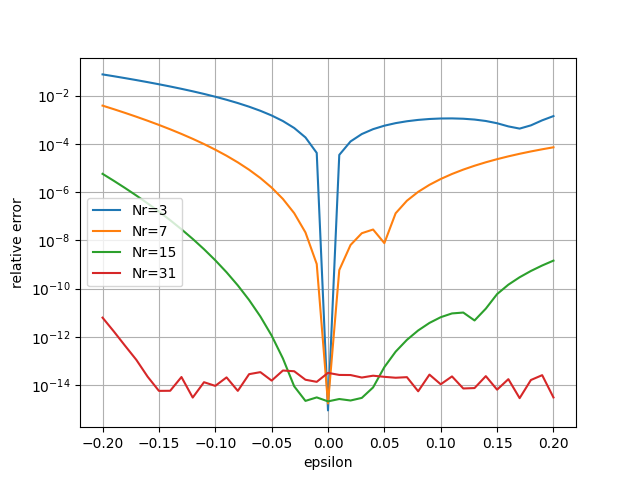
\includegraphics[width=0.48\textwidth]{fig/basis_1ev_grid.png}
	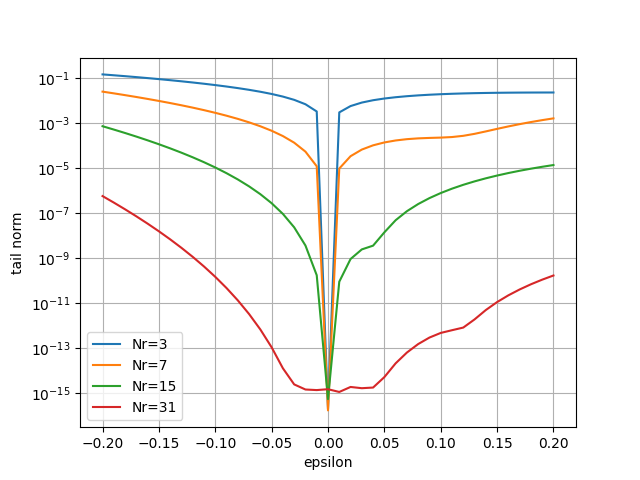
\includegraphics[width=0.48\textwidth]{fig/basis_1ev_tail.png}
	\caption{The left most figure shows the $f(v)$ expansion evaluated at uniform grid in the radial direction followed by normed difference computation for increasing $N_r$ polynomials. For a given Maxwellian distribution (i.e., $h^{\alpha}=1$) we compute the projection of the solution to $T_\beta=T_\alpha (1+\epsilon)$ with computed $W_{\beta\alpha}$, where $h^{\beta} = W_{\beta \alpha} h^{\alpha}$. The right most figure shows the tail of the computed $h^{\beta}$ with increasing polynomials in the radial direction.  \label{fig:basis_projection_error}
	}
\end{figure}
\begin{figure}[!hbtp]
	\centering
	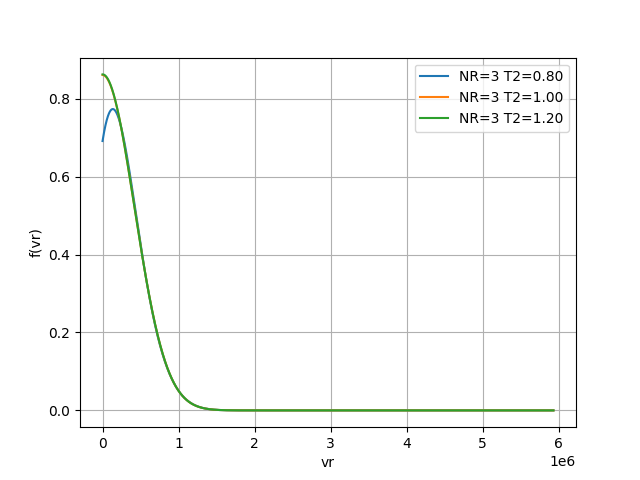
\includegraphics[width=0.48\textwidth]{fig/basis_1ev_f_NR_3.png}
	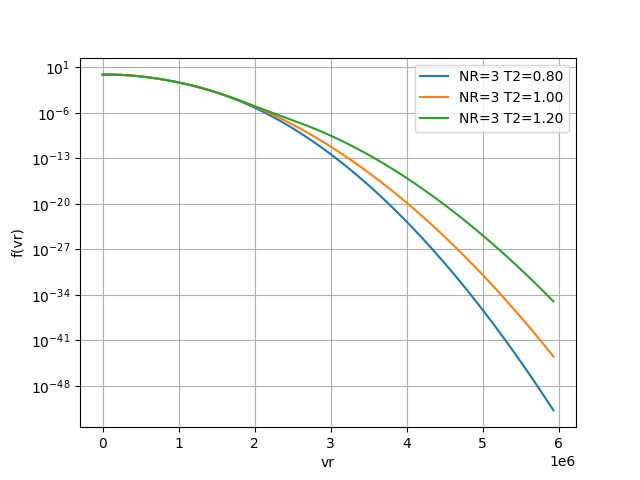
\includegraphics[width=0.48\textwidth]{fig/basis_1ev_log_f_NR_3.png}
	
	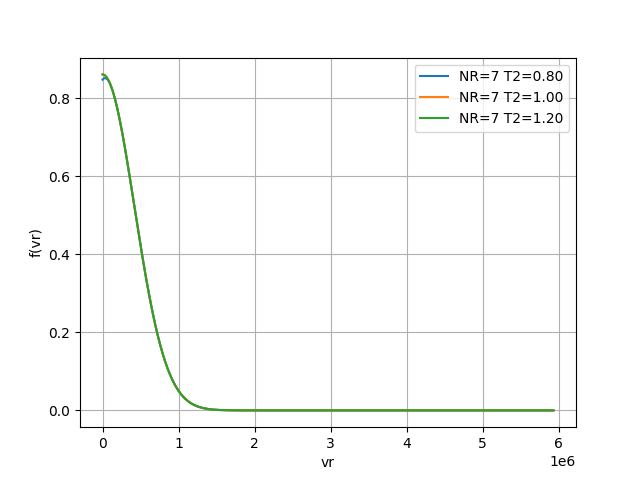
\includegraphics[width=0.48\textwidth]{fig/basis_1ev_f_NR_7.png}
	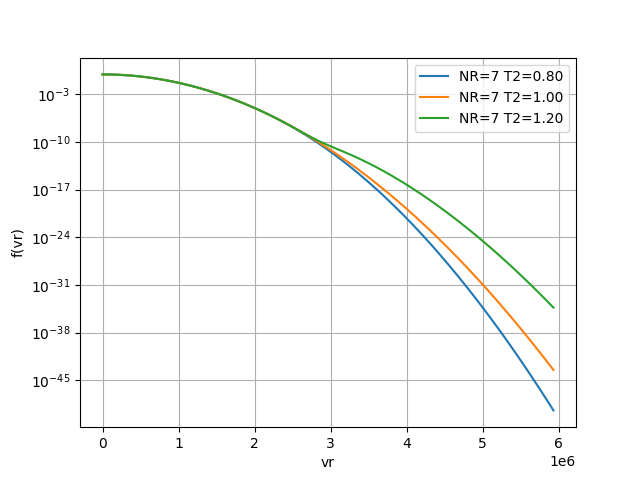
\includegraphics[width=0.48\textwidth]{fig/basis_1ev_log_f_NR_7.png}
	
	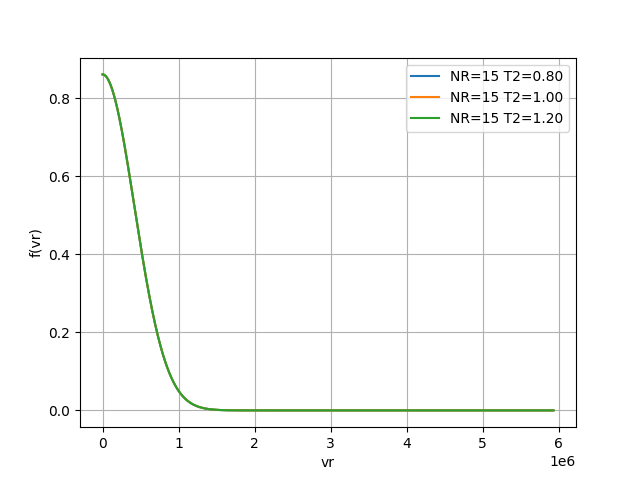
\includegraphics[width=0.48\textwidth]{fig/basis_1ev_f_NR_15.png}
	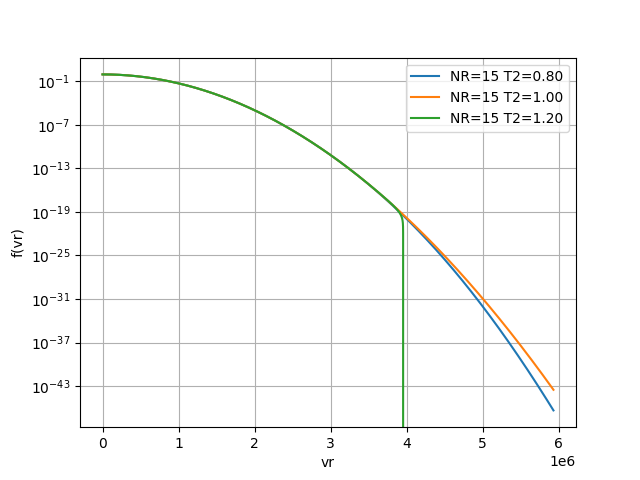
\includegraphics[width=0.48\textwidth]{fig/basis_1ev_log_f_NR_15.png}

	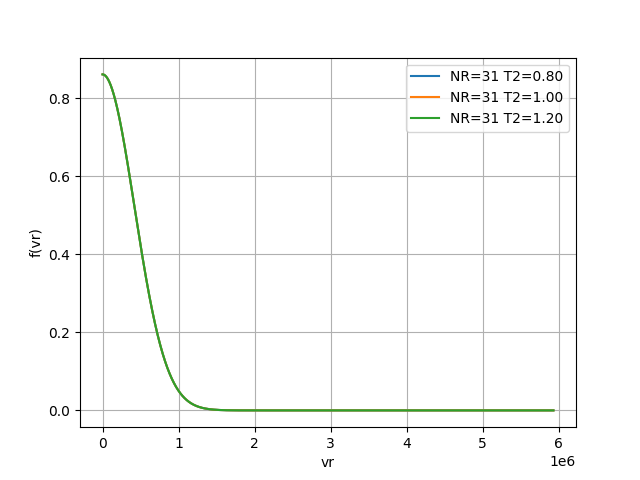
\includegraphics[width=0.48\textwidth]{fig/basis_1ev_f_NR_31.png}
	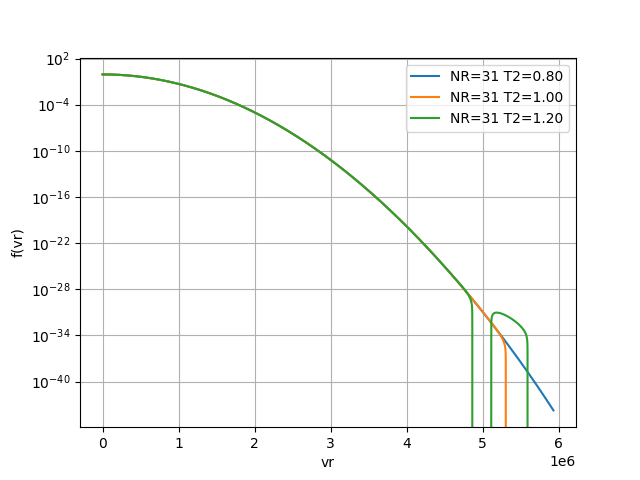
\includegraphics[width=0.48\textwidth]{fig/basis_1ev_log_f_NR_31.png}
	\caption{ For each row the the right most figure shows the log scale to emphasis the variation in the tails of the distribution function. Each row corresponds to a temperature change indicated byt the $\epsilon$ parameter, and projected coefficient evaluated at a uniformly space grid of $10^5$ points in the range of $(0,6V_th)$. 
		\label{fig:basis_grid_plot}
	}
\end{figure}


\newpage
\section{Numerical results with picewise linear synthetic cross section data}
Experimental setup summary. 
\begin{itemize}
	\item Collision operator assembled using composite Simpson rule with 1601 points in the radial direction. 
\end{itemize}
\begin{figure}[!tbhp]
	\centering
	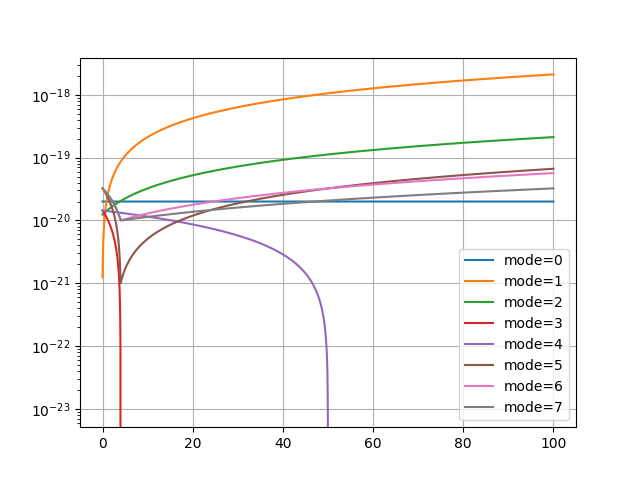
\includegraphics[width=0.8\textwidth]{fig/dat_1ev_cs.png}
	\caption{Total cross-section plots with different synthetic functions. For modes 3,4,5,6 the kink is at an exact quadrature point while mode 7 kink location is not co-located with a quadrature point. For all the experiment differential cross-section computed with uniform distribution.}
\end{figure}
\begin{figure}[!htbp]
	\centering
	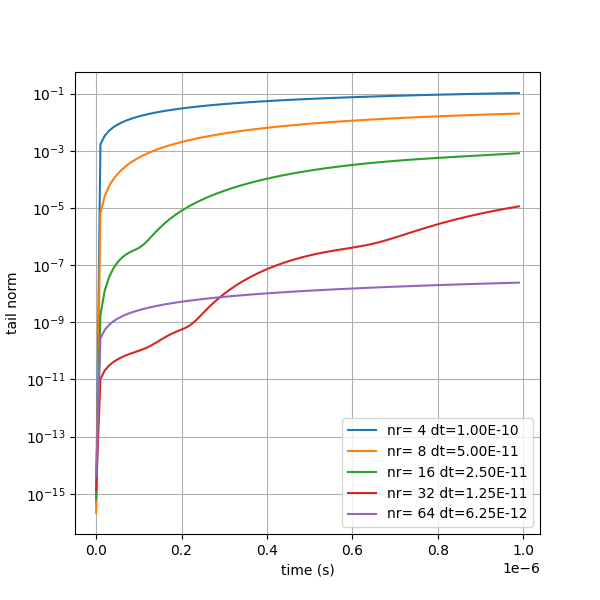
\includegraphics[width=0.32\textwidth]{fig/dat_1ev_cs_m0_tail.png}
	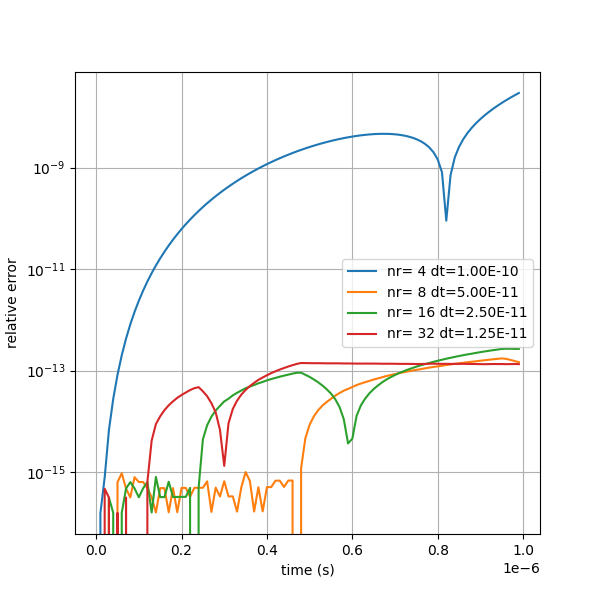
\includegraphics[width=0.32\textwidth]{fig/dat_1ev_cs_m0_temp_error.png}
	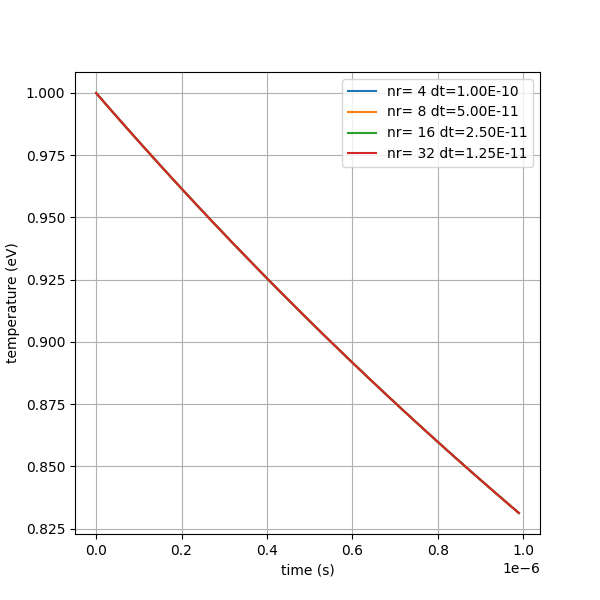
\includegraphics[width=0.32\textwidth]{fig/dat_1ev_cs_m0_temp.png}
	\caption{Mode 0}
\end{figure}
\begin{figure}[!htbp]
	\centering
	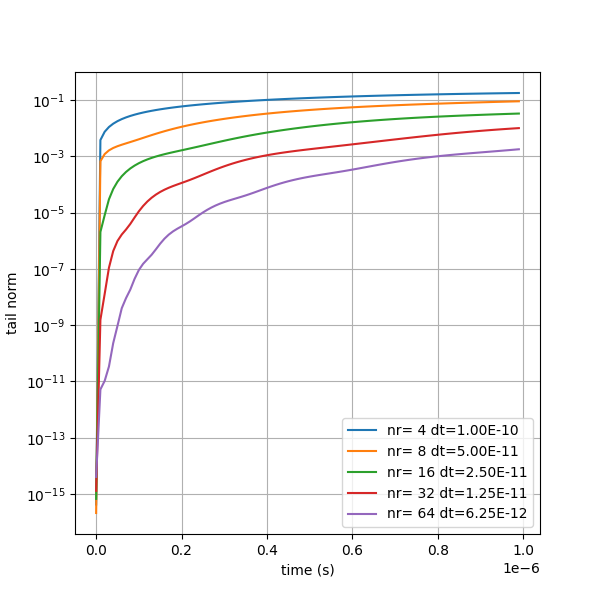
\includegraphics[width=0.32\textwidth]{fig/dat_1ev_cs_m1_tail.png}
	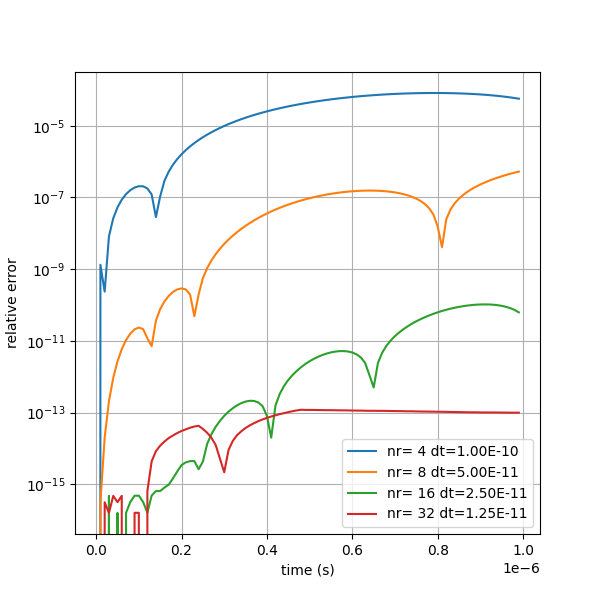
\includegraphics[width=0.32\textwidth]{fig/dat_1ev_cs_m1_temp_error.png}
	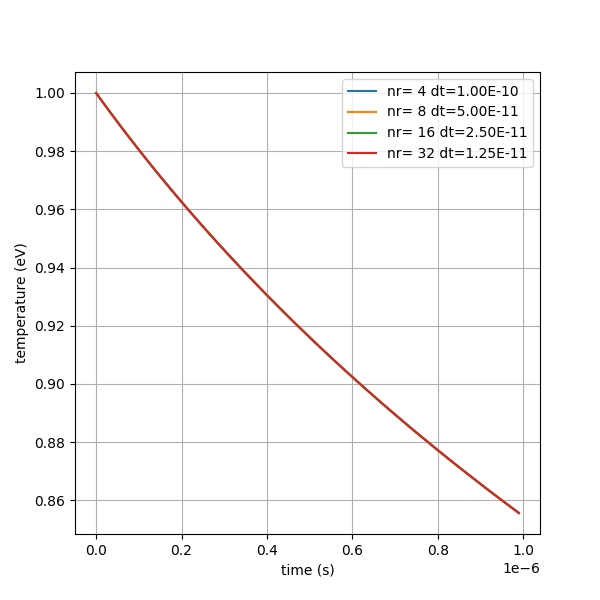
\includegraphics[width=0.32\textwidth]{fig/dat_1ev_cs_m1_temp.png}
	\caption{Mode 1}
\end{figure}
\begin{figure}[!htbp]
	\centering
	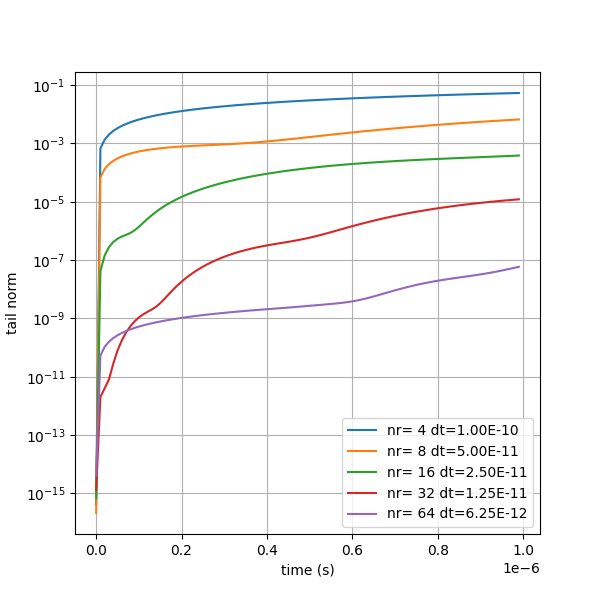
\includegraphics[width=0.32\textwidth]{fig/dat_1ev_cs_m2_tail.png}
	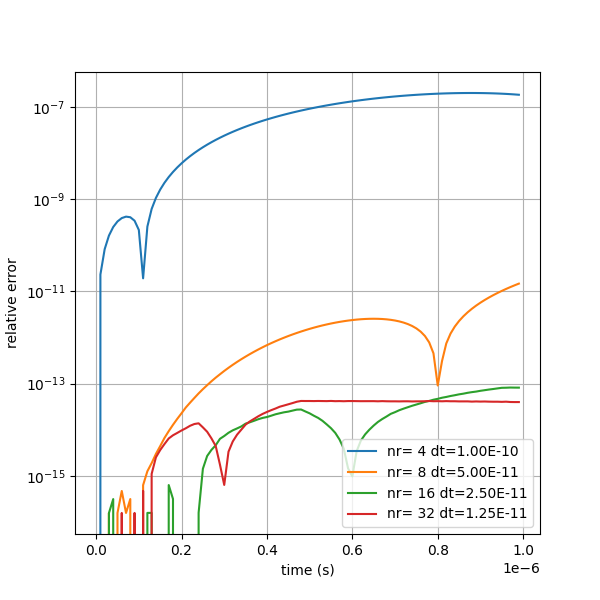
\includegraphics[width=0.32\textwidth]{fig/dat_1ev_cs_m2_temp_error.png}
	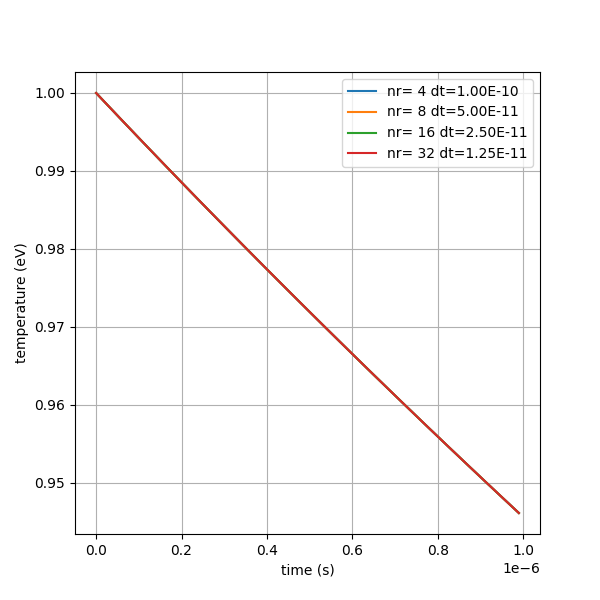
\includegraphics[width=0.32\textwidth]{fig/dat_1ev_cs_m2_temp.png}
	\caption{Mode 2}
\end{figure}
\begin{figure}[!htbp]
	\centering
	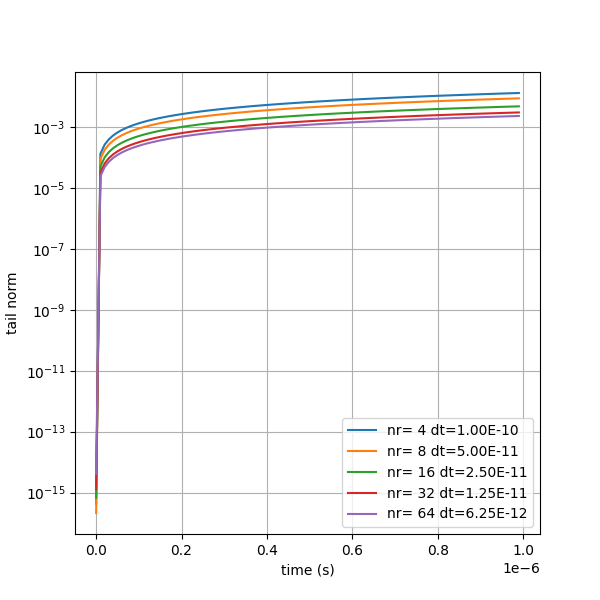
\includegraphics[width=0.32\textwidth]{fig/dat_1ev_cs_m3_tail.png}
	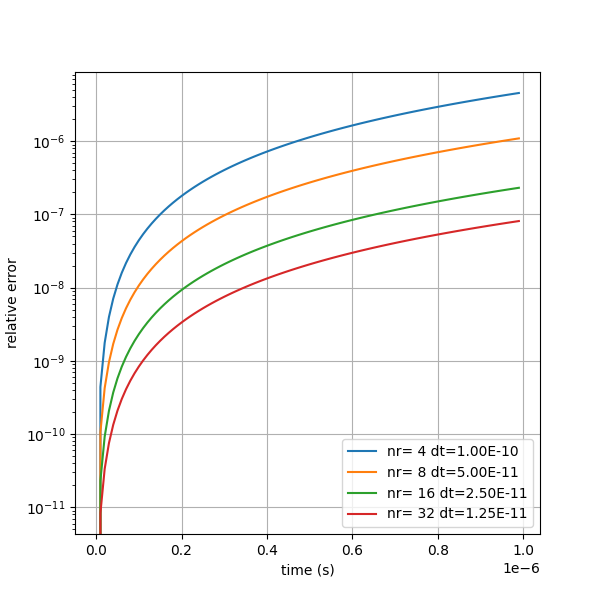
\includegraphics[width=0.32\textwidth]{fig/dat_1ev_cs_m3_temp_error.png}
	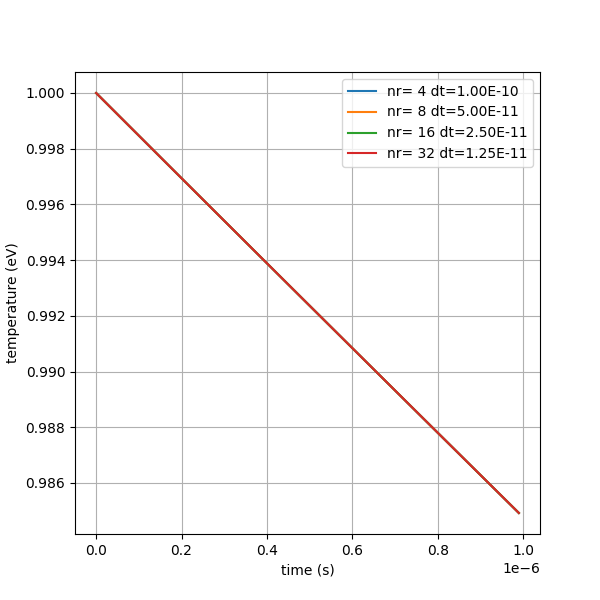
\includegraphics[width=0.32\textwidth]{fig/dat_1ev_cs_m3_temp.png}
	\caption{Mode 3}
\end{figure}
\begin{figure}[!htbp]
	\centering
	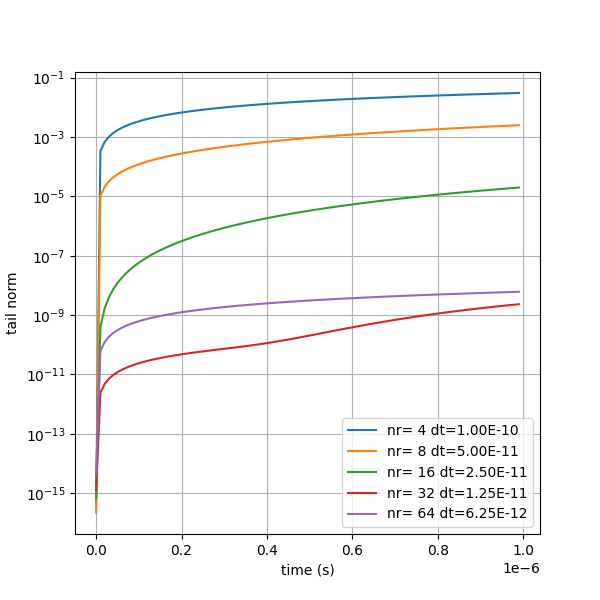
\includegraphics[width=0.32\textwidth]{fig/dat_1ev_cs_m4_tail.png}
	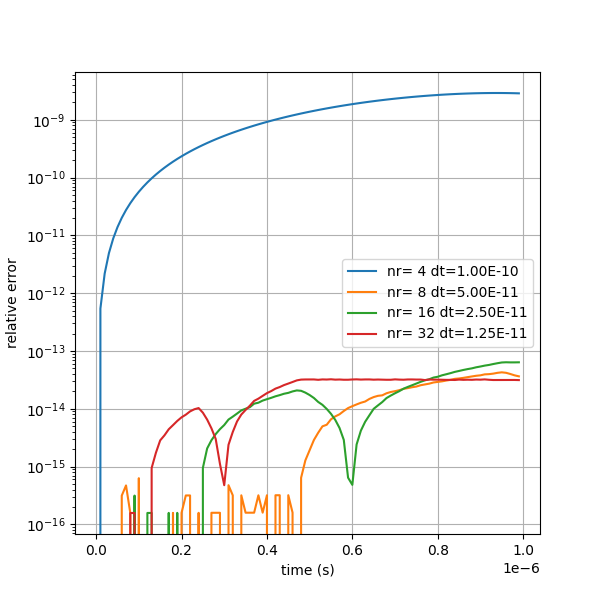
\includegraphics[width=0.32\textwidth]{fig/dat_1ev_cs_m4_temp_error.png}
	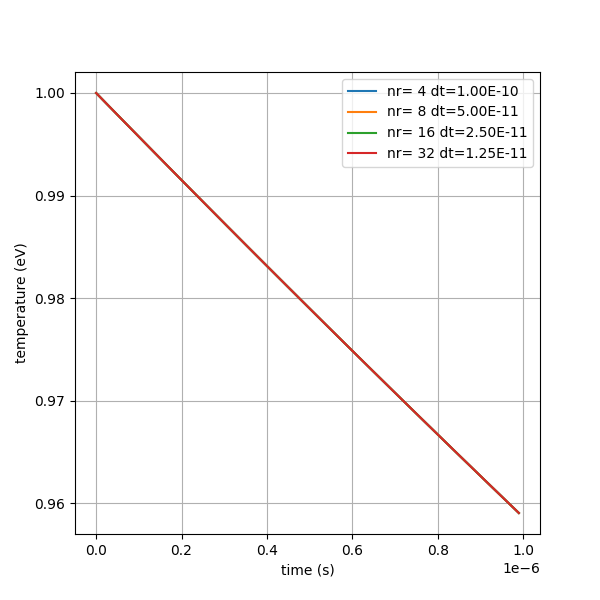
\includegraphics[width=0.32\textwidth]{fig/dat_1ev_cs_m4_temp.png}
	\caption{Mode 4}
\end{figure}
\begin{figure}[!htbp]
	\centering
	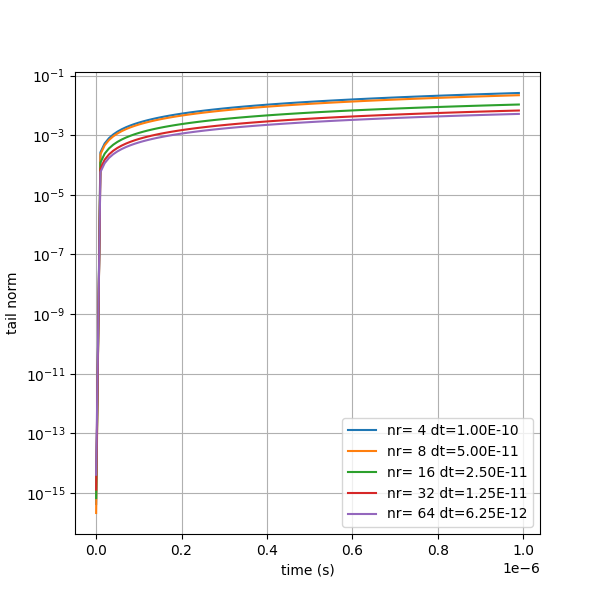
\includegraphics[width=0.32\textwidth]{fig/dat_1ev_cs_m5_tail.png}
	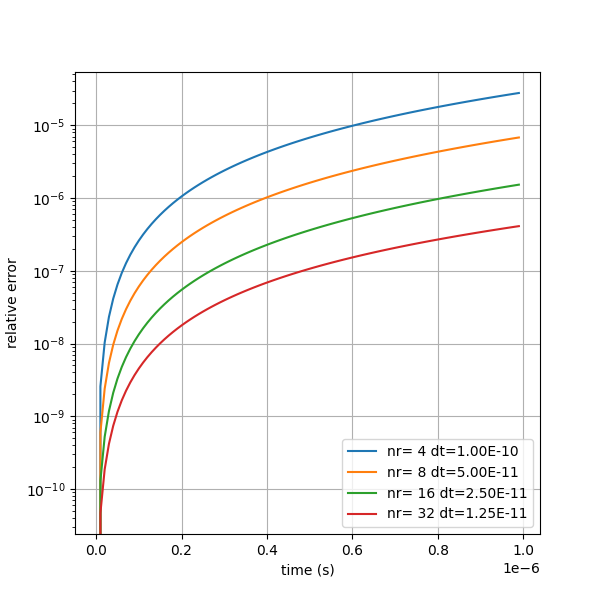
\includegraphics[width=0.32\textwidth]{fig/dat_1ev_cs_m5_temp_error.png}
	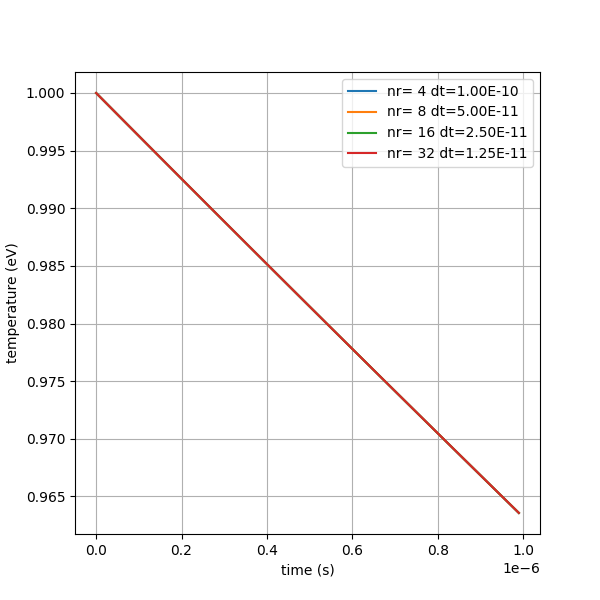
\includegraphics[width=0.32\textwidth]{fig/dat_1ev_cs_m5_temp.png}
	\caption{Mode 5}
\end{figure}
\begin{figure}[!htbp]
	\centering
	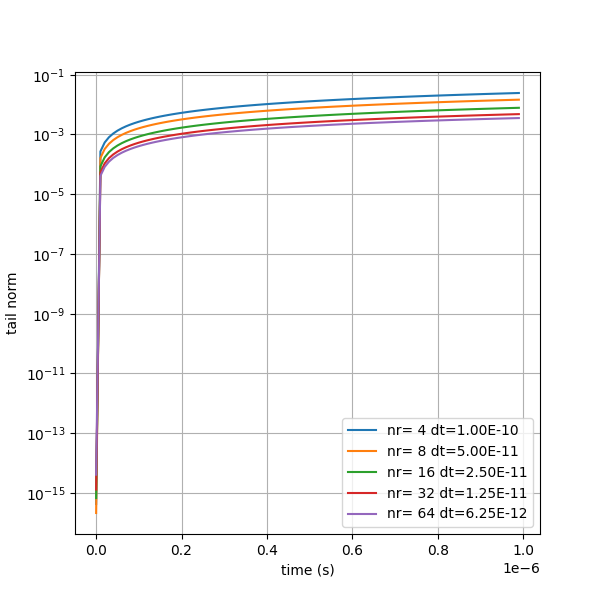
\includegraphics[width=0.32\textwidth]{fig/dat_1ev_cs_m6_tail.png}
	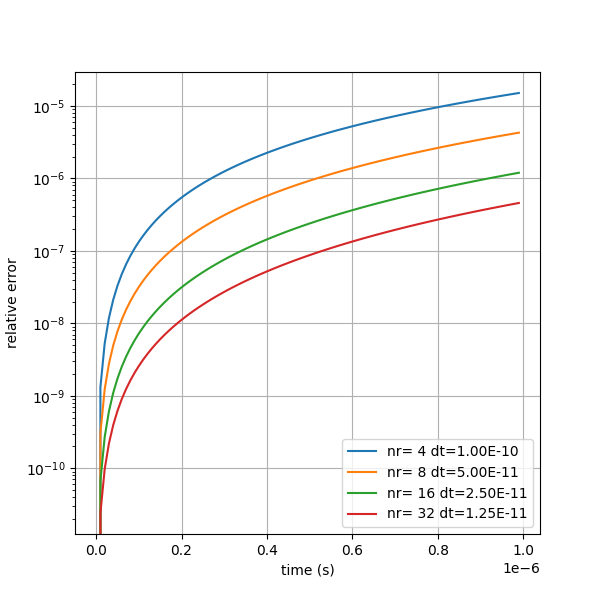
\includegraphics[width=0.32\textwidth]{fig/dat_1ev_cs_m6_temp_error.png}
	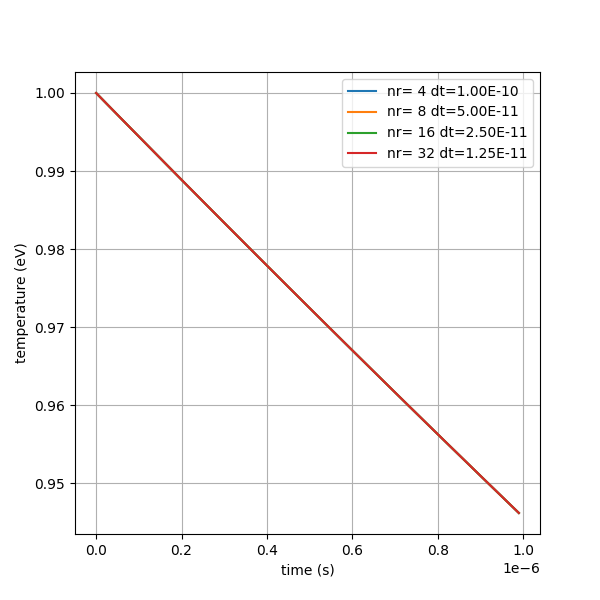
\includegraphics[width=0.32\textwidth]{fig/dat_1ev_cs_m6_temp.png}
	\caption{Mode 6}
\end{figure}
\begin{figure}[!htbp]
	\centering
	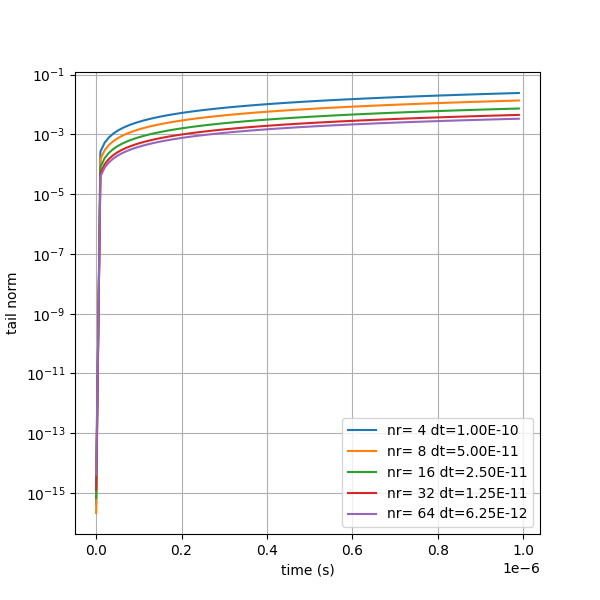
\includegraphics[width=0.32\textwidth]{fig/dat_1ev_cs_m7_tail.png}
	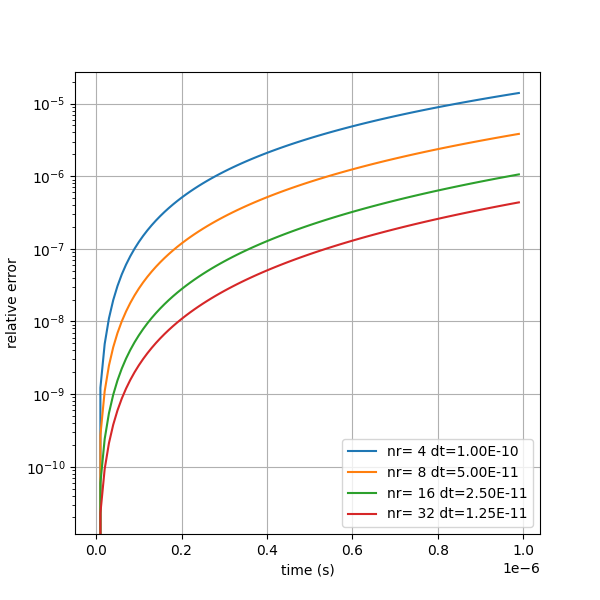
\includegraphics[width=0.32\textwidth]{fig/dat_1ev_cs_m7_temp_error.png}
	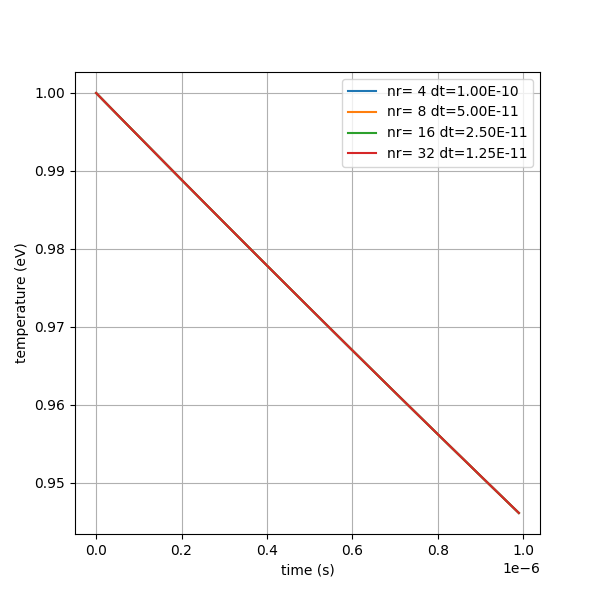
\includegraphics[width=0.32\textwidth]{fig/dat_1ev_cs_m7_temp.png}
	\caption{Mode 7}
\end{figure}


\bibliographystyle{plain}
\bibliography{bte_notes.bib}


\newpage
\appendix
\section{Derivation of Collision operators}
\subsection{Binary reactions}
\label{subsec:binary_reactions}
We start with reactions of the type
\begin{align*}
\text{Ar} + e \longrightarrow X + e
\end{align*}
where $X = \text{Ar}$ in the case of elastic collisions and $X = \text{Ar}^\ast$ in the case of excitation events. Let us denote the expressions that map given pre-collisional velocities $\vect{v}_e$, $\vect{v}_0$ to post-collisional velocities as 
\begin{align*}
\vect{v}_e^\text{post} &= \vect{v}_e^\text{post} \of{\vect{v}_e, \vect{v}_0, \vect{\omega}}
\\
\vect{v}_0^\text{post} &= \vect{v}_0^\text{post} \of{\vect{v}_e, \vect{v}_0, \vect{\omega}}
\end{align*} 
where $\vect{\omega} \in S^2$ is the vector defining along which directions velocities change in the reaction. Specifically, from the conservation of momentum and energy it can be derived that
\begin{align*}
\vect{v}_e^\text{post} &= \vect{v}_e + \frac{\alpha}{m_e}\vect{\omega},
\\
\vect{v}_0^\text{post} &= \vect{v}_0 - \frac{\alpha}{m_0}\vect{\omega},
\end{align*}
where
\begin{align*}
\alpha &= \frac{u + \sqrt{u^2 - 4 \Delta E \mu}}{2\mu},
\quad 
u = \vect{\omega} \cdot \left( \vect{v}_0 - \vect{v}_e \right),
\quad 
\mu = \frac{m_e+m_0}{2 m_e m_0}
\end{align*}
and $\Delta E$ denotes the energy loss during the reaction ($\Delta E = 0$ for elastic collisions). Note that if $\Delta E=0$, then
\begin{align*}
\vect{v}_e^\text{post} \of{\vect{v}_e, \vect{v}_0, \vect{\omega}} = \vect{v}_e,
\\
\vect{v}_0^\text{post} \of{\vect{v}_e, \vect{v}_0, \vect{\omega}} = \vect{v}_0,
\end{align*} 
for $\vect{\omega} \cdot \left( \vect{v}_0 - \vect{v}_e \right) < 0$, that is, no collision happens.

The inverse map (assuming it exists and well-defined) is denoted as 
\begin{align*}
\vect{v}_e^\text{pre} &= \vect{v}_e^\text{pre} \of{\vect{v}_e, \vect{v}_0, \vect{\omega}}
\\
\vect{v}_0^\text{pre} &= \vect{v}_0^\text{pre} \of{\vect{v}_e, \vect{v}_0, \vect{\omega}}
\end{align*} 
where $\vect{v}_e$, $\vect{v}_0$ now represent the post-collision velocities. Thus we have 
\begin{align*}
\vect{v}_e &= \vect{v}_e^\text{pre} \of{\vect{v}_e^\text{post} \of{\vect{v}_e, \vect{v}_0, \vect{\omega}}, \vect{v}_0^\text{post} \of{\vect{v}_e, \vect{v}_0, \vect{\omega}}, \vect{\omega}}
\\
\vect{v}_0 &= \vect{v}_0^\text{pre} \of{\vect{v}_e^\text{post} \of{\vect{v}_e, \vect{v}_0, \vect{\omega}}, \vect{v}_0^\text{post} \of{\vect{v}_e, \vect{v}_0, \vect{\omega}}, \vect{\omega}}
\end{align*} 

Let us denote the collision kernel of reaction as $B\of{\vect{v}_e, \vect{v}_0, \vect{\omega}}$ which is a function of pre-collision velocities $\vect{v}_e$, $\vect{v}_0$ and the direction of velocity change $\vect{\omega}$. The number of electrons with velocity $\vect{v}_e$ that will participate in the reaction and, thus, lost is given by 
\begin{align*}
C^- = \myint_{R^3} \myint_{S^2} B\of{\vect{v}_e, \vect{v}_0, \vect{\omega}} f_e\of{\vect{v}_e} f_0\of{\vect{v}_0} \diff{\vect{v}_0} \diff{\vect{\omega}}
\end{align*}
The number of electrons with the same velocity created in the reaction is given by
\begin{align*}
C^+ = \myint_{R^3} \myint_{R^3} \myint_{S^2} 
B\of{\vect{v}_e^\prime, \vect{v}_0^\prime, \vect{\omega}} 
f_e\of{\vect{v}_e^\prime} f_0\of{\vect{v}_0^\prime} 
\delta\of{\vect{v}_e^\text{post}\of{\vect{v}_e^\prime, \vect{v}_0^\prime, \vect{\omega}} - \vect{v}_e} 
\diff{\vect{v}_0^\prime} \diff{\vect{v}_e^\prime} \diff{\vect{\omega}}
\end{align*}
where we integrate over all possible pre-collision velocities $\vect{v}_e^\prime$, $\vect{v}_0^\prime$ but pick out only those that result in post-collision electron velocity $\vect{v}_e$ (thanks to the delta function). Note that in the expression for $C^-$ symbols $\vect{v}_e$, $\vect{v}_0$ have the meaning of pre-collision velocity, while in the expression for $C^+$ those are denoted by $\vect{v}_e^\prime$, $\vect{v}_0^\prime$. 

\textbf{Remark.} One could define $C^-$ in an analogous to $C^+$ way. That is, consider reactions for all possible pre-collision velocities $\vect{v}_e^\prime$, $\vect{v}_0^\prime$ but select only those that lead to loss of electrons with velocity $\vect{v}_e$
\begin{align*}
C^- = \myint_{R^3} \myint_{R^3} \myint_{S^2} 
B\of{\vect{v}_e^\prime, \vect{v}_0^\prime, \vect{\omega}} 
f_e\of{\vect{v}_e^\prime} f_0\of{\vect{v}_0^\prime} 
\delta\of{\vect{v}_e^\prime - \vect{v}_e} 
\diff{\vect{v}_0^\prime} \diff{\vect{v}_e^\prime} \diff{\vect{\omega}}.
\end{align*}

We understand $C^-$ and $C^+$ as operators acting on functions of variable $\vect{v}_e$. Their weak forms are given by
\begin{align*}
\myint_{R^3} C^- \phi\of{\vect{v}_e} \diff{\vect{v}_e} 
&=
\myint_{R^3} \myint_{R^3} \myint_{S^2} 
B\of{\vect{v}_e, \vect{v}_0, \vect{\omega}} 
f_e\of{\vect{v}_e} f_0\of{\vect{v}_0} 
\phi\of{\vect{v}_e} 
\diff{\vect{v}_e} \diff{\vect{v}_0} \diff{\vect{\omega}}
\\
\myint_{R^3} C^+ \phi\of{\vect{v}_e} \diff{\vect{v}_e} 
&= 
\myint_{R^3} \myint_{R^3} \myint_{S^2} 
B\of{\vect{v}_e^\prime, \vect{v}_0^\prime, \vect{\omega}} 
f_e\of{\vect{v}_e^\prime} f_0\of{\vect{v}_0^\prime} 
\phi\of{\vect{v}_e^\text{post}\of{\vect{v}_e^\prime, \vect{v}_0^\prime, \vect{\omega}}} 
\diff{\vect{v}_0^\prime} \diff{\vect{v}_e^\prime} \diff{\vect{\omega}}
\\
&= 
\myint_{R^3} \myint_{R^3} \myint_{S^2} 
B\of{\vect{v}_e, \vect{v}_0, \vect{\omega}} 
f_e\of{\vect{v}_e} f_0\of{\vect{v}_0} 
\phi\of{\vect{v}_e^\text{post}\of{\vect{v}_e, \vect{v}_0, \vect{\omega}}} 
\diff{\vect{v}_0} \diff{\vect{v}_e} \diff{\vect{\omega}}
\end{align*}
where we integrated out the delta function and renamed dummy variables. Thus the weak form of the total collision operator $C = C^+ - C^-$ can be written as 
\begin{align*}
\myint_{R^3} C \phi\of{\vect{v}_e} \diff{\vect{v}_e} 
&=
\myint_{R^3} \myint_{R^3} \myint_{S^2} 
B\of{\vect{v}_e, \vect{v}_0, \vect{\omega}} 
f_e\of{\vect{v}_e} f_0\of{\vect{v}_0} 
\left(
\phi\of{\vect{v}_e^\text{post}\of{\vect{v}_e, \vect{v}_0, \vect{\omega}}} 
- \phi\of{\vect{v}_e} 
\right)
\diff{\vect{v}_0} \diff{\vect{v}_e} \diff{\vect{\omega}}
\end{align*}

While for our purposes this formulation is all we need, for completeness sake we derive a strong form of the collision operator. To do so, we perform a change of variables in the weak form of gain operator $C^+$ according to:
\begin{align*}
\vect{v}_e^\prime &= \vect{v}_e^\text{pre} \of{\vect{v}_e^{\prime\prime}, \vect{v}_0^{\prime\prime}, \vect{\omega}}
\\
\vect{v}_0^\prime &= \vect{v}_0^\text{pre} \of{\vect{v}_e^{\prime\prime}, \vect{v}_0^{\prime\prime}, \vect{\omega}}
\end{align*}
As result we get
\begin{multline*}
\myint_{R^3} C^+ \phi\of{\vect{v}_e} \diff{\vect{v}_e} 
= 
\myint_{R^3} \myint_{R^3} \myint_{S^2} 
B\of{\vect{v}_e^\text{pre} \of{\vect{v}_e^{\prime\prime}, \vect{v}_0^{\prime\prime}, \vect{\omega}}, \vect{v}_0^\text{pre} \of{\vect{v}_e^{\prime\prime}, \vect{v}_0^{\prime\prime}, \vect{\omega}}, \vect{\omega}} 
\times
\\
\times
f_e\of{\vect{v}_e^\text{pre} \of{\vect{v}_e^{\prime\prime}, \vect{v}_0^{\prime\prime}, \vect{\omega}}} 
f_0\of{\vect{v}_0^\text{pre} \of{\vect{v}_e^{\prime\prime}, \vect{v}_0^{\prime\prime}, \vect{\omega}}} 
\phi\of{\vect{v}_e^{\prime\prime}} 
|J\of{\vect{v}_e^{\prime\prime}, \vect{v}_0^{\prime\prime}, \vect{\omega}}|
\diff{\vect{v}_0^{\prime\prime}} \diff{\vect{v}_e^{\prime\prime}} \diff{\vect{\omega}}
\end{multline*}
or, after renaming dummy variables,
\begin{multline*}
\myint_{R^3} C^+ \phi\of{\vect{v}_e} \diff{\vect{v}_e} 
= 
\myint_{R^3} \myint_{R^3} \myint_{S^2} 
B\of{\vect{v}_e^\text{pre} \of{\vect{v}_e, \vect{v}_0, \vect{\omega}}, \vect{v}_0^\text{pre} \of{\vect{v}_e, \vect{v}_0, \vect{\omega}}, \vect{\omega}} 
\times
\\
\times
f_e\of{\vect{v}_e^\text{pre} \of{\vect{v}_e, \vect{v}_0, \vect{\omega}}} 
f_0\of{\vect{v}_0^\text{pre} \of{\vect{v}_e, \vect{v}_0, \vect{\omega}}} 
\phi\of{\vect{v}_e} 
|J\of{\vect{v}_e, \vect{v}_0, \vect{\omega}}|
\diff{\vect{v}_0} \diff{\vect{v}_e} \diff{\vect{\omega}}
\end{multline*}
where $J\of{\vect{v}_e, \vect{v}_0, \vect{\omega}} = \frac{ \partial \left( \vect{v}_e^\text{pre}\of{\vect{v}_e, \vect{v}_0, \vect{\omega}}, \vect{v}_0^\text{pre}\of{\vect{v}_e, \vect{v}_0, \vect{\omega}} \right)}{\partial \left( \vect{v}_e, \vect{v}_0 \right)}$ is the Jacobian of the transformation of variables. Note that in this last expression $\vect{v}_e$, $\vect{v}_0$ can be interpreted as post-collision velocities. Combining it with the weak form of the loss operator (where $\vect{v}_e$, $\vect{v}_0$ actually stand for pre-collision velocities) we obtain
\begin{multline*}
\myint_{R^3} C \phi\of{\vect{v}_e} \diff{\vect{v}_e} 
=
\myint_{R^3} \myint_{R^3} \myint_{S^2} 
\phi\of{\vect{v}_e} 
\diff{\vect{v}_0} \diff{\vect{v}_e} \diff{\vect{\omega}}
\times
\\
\times
\big(
B^\text{pre}\of{\vect{v}_e, \vect{v}_0, \vect{\omega}}  
f_e^\text{pre}\of{\vect{v}_e, \vect{v}_0, \vect{\omega}}
f_0^\text{pre}\of{\vect{v}_e, \vect{v}_0, \vect{\omega}} 
|J\of{\vect{v}_e, \vect{v}_0, \vect{\omega}}|
\\
-
B\of{\vect{v}_e, \vect{v}_0, \vect{\omega}} 
f_e\of{\vect{v}_e} f_0\of{\vect{v}_0} 
\big)
\end{multline*}
where notation $x^\text{pre}\of{\vect{v}_e, \vect{v}_0, \vect{\omega}} = x\of{\vect{v}_e^\text{pre} \of{\vect{v}_e, \vect{v}_0, \vect{\omega}}, \vect{v}_0^\text{pre} \of{\vect{v}_e, \vect{v}_0, \vect{\omega}}, \vect{\omega}}$ is used. Thus, a strong form of the total collision operator for general binary reactions can be written as
\begin{align*}
C = 
\myint_{R^3} \myint_{S^2} 
\left(
f_e^\text{pre}
f_0^\text{pre}
B^\text{pre} 
|J|
-
f_e
f_0
B
\right)
\diff{\vect{v}_0} \diff{\vect{\omega}}
\end{align*}
In case of elastic collisions it can be shown that $|J| = 1$ and
\begin{align*}
B^\text{pre}\of{\vect{v}_e, \vect{v}_0, \vect{\omega}} &=
B\of{\vect{v}_e^\text{pre} \of{\vect{v}_e, \vect{v}_0, \vect{\omega}}, \vect{v}_0^\text{pre} \of{\vect{v}_e, \vect{v}_0, \vect{\omega}}, \vect{\omega}} 
\\
&=
B\of{|\vect{v}_e^\text{pre}- \vect{v}_0^\text{pre}|, |\left(\vect{v}_e^\text{pre}- \vect{v}_0^\text{pre}\right)\cdot\vect{\omega}|} 
\\
&=
B\of{|\vect{v}_e- \vect{v}_0|, |\left(\vect{v}_e- \vect{v}_0\right)\cdot\vect{\omega}|}
\\
&=
B\of{\vect{v}_e, \vect{v}_0, \vect{\omega}} 
\end{align*}
and the collision operator becomes the familiar
\begin{align*}
C = 
\myint_{R^3} \myint_{S^2} 
\left(
f_e^\text{pre}
f_0^\text{pre}
-
f_e
f_0
\right)
B
\diff{\vect{v}_0} \diff{\vect{\omega}}
\end{align*}

In the derivation above we assumed that the collision kernel $B=B\of{\vect{v}_e, \vect{v}_0, \vect{\omega}}$ is known. However, for electron-heavy particle collisions information is available in terms of collisional cross sections $\sigma = \sigma\of{|\vect{v}_e|, \chi, \theta}$, where $\vect{v}_e$ is the velocity of the incident electron in the frame of reference of the heavy particle, and $\chi$, $\theta$ are angles of scattering. It is usually assumed that collisions occur axisymmetrically, that is $\sigma = \sigma\of{|\vect{v}_e|, \chi}$

\begin{align*}
C^- = \myint_{R^3} \myint_{R^3} \myint_{0}^{\pi} \myint_{0}^{2\pi} 
|\vect{v}_e^\prime-\vect{v}_0^\prime| \sigma\of{|\vect{v}_e^\prime-\vect{v}_0^\prime|, \chi}
f_e\of{\vect{v}_e^\prime} f_0\of{\vect{v}_0^\prime} 
\delta\of{\vect{v}_e^\prime - \vect{v}_e} 
\diff{\vect{v}_0^\prime} \diff{\vect{v}_e^\prime} \sin\of{\chi} \diff{\chi} \diff{\theta}.
\end{align*}
\begin{align*}
C^+ = \myint_{R^3} \myint_{R^3} \myint_{0}^{\pi} \myint_{0}^{2\pi} 
|\vect{v}_e^\prime-\vect{v}_0^\prime| \sigma\of{|\vect{v}_e^\prime-\vect{v}_0^\prime|, \chi}
f_e\of{\vect{v}_e^\prime} f_0\of{\vect{v}_0^\prime} 
\delta\of{\vect{v}_e^\text{post}\of{\vect{v}_e^\prime, \vect{v}_0^\prime, \chi, \theta} - \vect{v}_e} 
\diff{\vect{v}_0^\prime} \diff{\vect{v}_e^\prime} \sin\of{\chi} \diff{\chi} \diff{\theta}.
\end{align*}

\clearpage
\subsection{Ionization}
Let's consider the following ionization reaction. 
\begin{equation}
	e + Ar \rightarrow e + Ar^{+} + e
\end{equation}
For a given pre-collision velocities $\vect{v_e}, \vect{v_0}$, let $\vect{v}^{post}_e(\vect{v_e},\vect{v_0},\omega), \vect{v}^{post}_0(\vect{v_e},\vect{v_0},\omega)$, $\vect{u}^{post}_e(\vect{v_e},\vect{v_0},\omega)$ be the post velocity maps of the scattered, ionized $Ar$ and ejected electron.

Following the same derivation we can write the collision operator for ionization, 
\begin{align}
\myint_{R^3} C \phi\of{\vect{v}_e} \diff{\vect{v}_e} 
&=
\myint_{R^3} \myint_{R^3} \myint_{S^2} 
B\of{\vect{v}_e, \vect{v}_0, \vect{\omega}}
f_e\of{\vect{v}_e} f_0\of{\vect{v}_0} \times \\
&\left(
\phi\of{\vect{v}_e^\text{post}\of{\vect{v}_e, \vect{v}_0, \vect{\omega}}} +
\phi\of{\vect{u}_e^\text{post}\of{\vect{v}_e, \vect{v}_0, \vect{\omega}}} 
- \phi\of{\vect{v}_e} 
\right)
\diff{\vect{v}_0} \diff{\vect{v}_e} \diff{\vect{\omega}}
\end{align}  

\subsection{Recombination}
Let's consider the following recombination reaction. 
\begin{equation}
	e + Ar^{+} + e \rightarrow e + Ar
\end{equation}
Let $\vect{v}_e$, $\vect{v}_0$, and $\vect{u}_e$ be the velocities of the 3-body collision and the post collision velocities are given by $\vect{v}^{post}_e(\vect{v}_e,\vect{v}_0,\omega)$ and $\vect{v}^{post}_0(\vect{v}_e,\vect{v}_0,\omega)$.

\begin{align}
\myint_{R^3} C \phi\of{\vect{v}_e} \diff{\vect{v}_e} 
&=
\myint_{R^3} \myint_{R^3} \myint_{R^3} \myint_{S^2} 
B\of{\vect{v}_e, \vect{v}_0, \vect{\omega}} 
f_e\of{\vect{u}_e} f_e\of{\vect{v}_e} f_0\of{\vect{v}_0} \times \\
&\left(
\phi\of{\vect{v}_e^\text{post}\of{\vect{v}_e, \vect{v}_0, \vect{\omega}}} 
- \phi\of{\vect{v}_e} 
\right)
\diff{\vect{v}_0} \diff{\vect{u}_e} \diff{\vect{v}_e} \diff{\vect{\omega}}
\end{align}

\newpage
\subsection{Binary reactions II}

Let's consider the following reactions:
\begin{align*}
	e + Ar &\rightarrow e + Ar^{*} \\
	e + Ar^{*} &\rightarrow e + Ar
\end{align*}
Denote momenta of particles on one side of the reaction as $\vect{p}_e$ and $\vect{p}_0$ and on the other side as $\vect{p}_e^\prime$ and $\vect{p}_*$. Their total momenta, $\vect{K}_{e,0}$ and $\vect{K}_{e,*}$, and energies, $E_{e,0}$ and $E_{e, *}$, can be expressed as:
\begin{align*}
\vect{K}_{e,0} &= \vect{p}_0 + \vect{p}_e
\\
\vect{K}_{e,*} &= \vect{p}_* + \vect{p}_e^\prime
\\
E_{e,0} &= \frac{\vect{p}_0^2}{2M} + \frac{\vect{p}_e^2}{2m} 
= \frac{\vect{K}_{e,0}^2}{2M} + u_{e,0}
\\
E_{e,*} &= \frac{\vect{p}_*^2}{2M} + \frac{{\vect{p}_e^\prime}^2}{2m} 
= \frac{\vect{K}_{e,*}^2}{2M} + u_{e,*}
\end{align*}
where $m$ and $M$ are masses of an electron and $Ar$;$u_{e,0}$ and $u_{e,*}$ are the relative energies of Ar-electron and Ar$^*$-electron pairs, and $\mu_{e,0}$ is the reduced mass:
\begin{align*}
u_{e,0} &= \frac{\vect{k}_{e,0}^2}{2\mu_{e,0}}, \quad \mu_{e,0} = \frac{mM}{(m+M)}
\quad \left[ \approx m \right]
\\
u_{\te,*} &= \frac{\vect{k}_{\te,*}^2}{2\mu_{e,0}}
\\
\vect{k}_{e,0} &= \frac{M \vect{p}_e - m \vect{p}_0}{m+M} 
\quad \left[ \approx \vect{p}_{e} \right]
\\
\vect{k}_{\te,*} &= \frac{M \tilde{\vect{p}}_\te - m \vect{p}_*}{m+M} 
\quad \left[ \approx \tilde{\vect{p}}_{e} \right]
\end{align*}

The conservation of energy becomes:
\begin{align*}
u_{e,0} = u_{e,*} + \Delta E_i
\end{align*}

In case of the excitation process, for given incident momenta $\vect{p}_e$ and $\vect{p}_0$ (such that $u_{e,0} > \Delta E_i$) a collision can be specified by the direction of relative momentum $\hat{\vect{k}}_{e,*}$. Similarly, in case of the de-excitation process, for given incident momenta $\tilde{\vect{p}}_e$ and $\vect{p}_*$ a collision can be specified by just the direction of the relative momentum $\hat{\vect{k}}_{e,0}$.

Reaction rate for excitation process:
\begin{multline*}
d R_{ex} = \left( 2 \pi \planck \right)^2 
f_e\of{\vect{p}_e} d^3 \vect{p}_e f_0\of{\vect{p}_0} d^3 \vect{p}_0
d^3 \vect{p}_{\tilde{e}} d^3 \vect{p}_*
\\
\times
| T\of{\vect{p}_0, \vect{p}_e \leftrightarrow \vect{p}_*, \vect{p}_{\tilde{e}}} |^2
\delta\of{\vect{K}_{e,0} - \vect{K}_{e,*}} 
\delta\of{E_{e,0} - E_{e,*} - \Delta E_i}
\end{multline*}

Reaction rate for de-excitation process:
\begin{multline*}
d R_{de} = \left( 2 \pi \planck \right)^2 
f_e\of{\vect{p}_{\tilde{e}}} d^3 \vect{p}_{\tilde{e}} f_*\of{\vect{p}_*} d^3 \vect{p}_*
d^3 \vect{p}_{e} d^3 \vect{p}_0
\\
\times
| T\of{\vect{p}_0, \vect{p}_e \leftrightarrow \vect{p}_*, \vect{p}_{\tilde{e}}} |^2
\delta\of{\vect{K}_{e,0} - \vect{K}_{\tilde{e},*}} 
\delta\of{E_{e,0} - E_{\tilde{e},*} - \Delta E_i}
\end{multline*}

Rate of loss of electrons in $d^3 \vect{p}_e$ due to excitation reactions:
\begin{align*}
L_{ex}\of{\vect{p}_e} = \int_{\vect{p}_0} \int_{\vect{p}_*} \int_{\vect{p}_\te} d R_{ex}
\end{align*}

Rate of gain of electrons in $d^3 \vect{p}_e$ due to de-excitation reactions:
\begin{align*}
G_{de}\of{\vect{p}_e} = \int_{\vect{p}_0} \int_{\vect{p}_*} \int_{\vect{p}_\te} d R_{de}
\end{align*}

Rate of gain of electrons in $d^3 \vect{p}_\te$ due to excitation reactions:
\begin{align*}
G_{ex}\of{\vect{p}_\te} = \int_{\vect{p}_e} \int_{\vect{p}_0} \int_{\vect{p}_*} d R_{ex}
\end{align*}

Rate of loss of electrons in $d^3 \vect{p}_\te$ due to de-excitation reactions:
\begin{align*}
L_{de}\of{\vect{p}_\te} = \int_{\vect{p}_e} \int_{\vect{p}_0} \int_{\vect{p}_*} d R_{de}
\end{align*}


Projection of the total collision operator due to excitations onto a test function $\psi$:
\begin{multline*}
\left< C_{ex}, \psi \right> = 
\int_{\vect{p}_e} \int_{\vect{p}_0} 
\int_{\vect{p}_\te} \int_{\vect{p}_*}
d R_{ex} \left( \psi\of{\vect{p}_\te}  
- \psi\of{\vect{p}_e} \right)
\\
= (2\pi h)^2 
\int_{R^3} \int_{R^3} 
\int_{R^3} \int_{R^3}
d^3 \vect{p}_0 d^3 \vect{p}_e
d^3 \vect{p}_* d^3 \vect{p}_\te  
\delta\of{\vect{K}_{e,0} - \vect{K}_{\te,*}} 
\delta\of{E_{e,0} - E_{\te,*} - \Delta E_i}
\\
\times
\left( \psi\of{\vect{p}_\te} - \psi\of{\vect{p}_e} \right) 
f_0\of{\vect{p}_0} f_e\of{\vect{p}_e} 
| T\of{\vect{p}_0, \vect{p}_e \leftrightarrow \vect{p}_*, \vect{p}_\te} |^2
\end{multline*}

Projection of the total collision operator due to recombination onto a test function $\psi$:
\begin{multline*}
\left< C_{de}, \psi \right> = 
\int_{\vect{p}_e} \int_{\vect{p}_0} 
\int_{\vect{p}_\te} \int_{\vect{p}_*}
d R_{de} \left( \psi\of{\vect{p}_e} - \psi\of{\vect{p}_\te} \right)
\\
= (2\pi h)^2 
\int_{R^3} \int_{R^3} 
\int_{R^3} \int_{R^3}
d^3 \vect{p}_0 d^3 \vect{p}_e
d^3 \vect{p}_* d^3 \vect{p}_\te  
\delta\of{\vect{K}_{e,0} - \vect{K}_{\te,*}} 
\delta\of{E_{e,0} - E_{\te,*} - \Delta E_i}
\\
\times
\left( \psi\of{\vect{p}_e} - \psi\of{\vect{p}_\te} \right) 
f_*\of{\vect{p}_*} f_e\of{\vect{p}_\te} 
| T\of{\vect{p}_0, \vect{p}_e \leftrightarrow \vect{p}_*, \vect{p}_\te} |^2
\end{multline*}

It is convenient to integrate out delta functions by changing variable from $(\vect{p}_*, \vect{p}_\te)$ to $(\vect{K}_{\te,*}, \vect{k}_{\te,*})$ for excitation collisions, and from $(\vect{p}_0, \vect{p}_e)$ to $(\vect{K}_{e,0}, \vect{k}_{e,0})$ for de-excitation collisions: 
\begin{align*}
d^3 \vect{p}_* d^3 \vect{p}_\te 
&= d^3 \vect{K}_{\te,*} d^3 \vect{k}_{\te,*}
\\
&= d^3 \vect{K}_{\te,*} \mu_{e,0} k_{\te,*} d u_{\te,*} d \Omega\of{\hat{\vect{k}}_{\te,*}}
\\
d^3 \vect{p}_0 d^3 \vect{p}_e 
&= d^3 \vect{K}_{e,0} d^3 \vect{k}_{e,0}
\\
&= d^3 \vect{K}_{e,0} \mu_{e,0} k_{e,0} d u_{e,0} d \Omega\of{\hat{\vect{k}}_{e,0}}
\end{align*}

\begin{multline*}
\left< C_{ex}, \psi \right> = 
(2\pi h)^2 
\int_{R^3} \int_{R^3} 
\int_{S^2}
d^3 \vect{p}_0 d^3 \vect{p}_e
\mu_{e,0} k_{\te,*}^{post} d \Omega\of{\hat{\vect{k}}_{\te,*}}
\\
\times
\left( \psi\of{\vect{p}_\te^{post}} - \psi\of{\vect{p}_e} \right) 
f_0\of{\vect{p}_0} f_e\of{\vect{p}_e} 
| T\of{\vect{p}_0, \vect{p}_e \leftrightarrow \vect{p}_*^{post}, \vect{p}_\te^{post}} |^2
\end{multline*}
where integration with respect to $\vect{p}_0$ and $\vect{p}_e$ are limited by the condition $u_{e,0} > \Delta E_i$, and

\begin{multline*}
\left< C_{de}, \psi \right> = 
(2\pi h)^2 
\int_{S^2}
\int_{R^3} \int_{R^3}
\mu_{e,0} k_{e,0}^{post} d \Omega\of{\hat{\vect{k}}_{e,0}}
d^3 \vect{p}_* d^3 \vect{p}_\te  
\\
\times
\left( \psi\of{\vect{p}_e^{post}} - \psi\of{\vect{p}_\te} \right) 
f_*\of{\vect{p}_*} f_e\of{\vect{p}_\te} 
| T\of{\vect{p}_0^{post}, \vect{p}_e^{post} \leftrightarrow \vect{p}_*, \vect{p}_\te} |^2
\end{multline*}

\begin{align*}
k_{\te,*}^{post} &= \sqrt{2 \mu_{e,0} \left( u_{\te,0} - \Delta E_{ex} \right)}
\\
\vect{p}_\te^{post} &= k_{\te,*}^{post} \hat{\vect{k}}_{\te,*} + \frac{m}{m+M} \left( \vect{p}_e + \vect{p}_0 \right)
\\
k_{e,0}^{post} &= \sqrt{2 \mu_{e,0} \left( u_{\te,*} + \Delta E_{ex} \right)}
\\
\vect{p}_e^{post} &= k_{e,0}^{post} \hat{\vect{k}}_{e,0} + \frac{m}{m+M} \left( \vect{p}_\te + \vect{p}_* \right)
\end{align*}


\begin{align*}
\sigma_{ex,CM} \of{ \vect{k}_{e,0} \rightarrow \hat{\vect{k}}_{\te,*}} 
&= \frac{d\sigma}{d\Omega\of{\hat{\vect{k}}_{\te,*}}}
\\
&= \frac{j_{reacted}/j_{incident}}{d\Omega\of{\hat{\vect{k}}_{\te,*}}}
\end{align*}
The product of incident flux times target density:
\begin{align*}
j_{incident} = \frac{k_{e,0}}{\mu_{e,0}} f_e\of{\vect{p}_e} d^3 \vect{p}_e f_0\of{\vect{p}_0} d^3 \vect{p}_0
\end{align*}
Scattering events in a given direction:
\begin{multline*}
j_{reacted} = \int_{\vect{K}_{\te,*}} \int_{E_{\te,*}} d R_{ex}
\\
= (2\pi h)^2 
d^3 \vect{p}_0 d^3 \vect{p}_e
\mu_{e,0} k_{\te,*}^{post} d \Omega\of{\hat{\vect{k}}_{\te,*}}
f_0\of{\vect{p}_0} f_e\of{\vect{p}_e} 
| T\of{\vect{p}_0, \vect{p}_e \leftrightarrow \vect{p}_*^{post}, \vect{p}_\te^{post}} |^2
\end{multline*}

\begin{align*}
\sigma_{ex,CM} \of{ \vect{k}_{e,0} \rightarrow \hat{\vect{k}}_{\te,*}} 
= (2\pi h)^2 
\mu_{e,0}^2 \frac{k_{\te,*}^{post}}{k_{e,0}}
| T\of{\vect{p}_0, \vect{p}_e \leftrightarrow \vect{p}_*^{post}, \vect{p}_\te^{post}} |^2
\end{align*}

\begin{align*}
| T\of{\vect{p}_0, \vect{p}_e \leftrightarrow \vect{p}_*^{post}, \vect{p}_\te^{post}} |^2 = 
\frac{\sigma_{ex,CM} \of{ \vect{k}_{e,0} \rightarrow \hat{\vect{k}}_{\te,*}}} 
{(2\pi h)^2 \mu_{e,0}^2 \frac{k_{\te,*}^{post}}{k_{e,0}}}
\end{align*}

\begin{multline*}
\left< C_{ex}, \psi \right> = 
\int_{R^3} \int_{R^3} 
\int_{S^2}
d^3 \vect{p}_0 d^3 \vect{p}_e
d \Omega\of{\hat{\vect{k}}_{\te,*}}
\\
\times
\left( \psi\of{\vect{p}_\te^{post}} - \psi\of{\vect{p}_e} \right) 
f_0\of{\vect{p}_0} f_e\of{\vect{p}_e} 
\frac{k_{e,0}}{\mu_{e,0}}
\sigma_{ex,CM} \of{ \vect{k}_{e,0} \rightarrow \hat{\vect{k}}_{\te,*}}
\end{multline*}

\begin{multline*}
\left< C_{de}, \psi \right> = 
\int_{S^2}
\int_{R^3} \int_{R^3}
d \Omega\of{\hat{\vect{k}}_{e,0}}
d^3 \vect{p}_* d^3 \vect{p}_\te  
\\
\times
\left( \psi\of{\vect{p}_e^{post}} - \psi\of{\vect{p}_\te} \right) 
f_*\of{\vect{p}_*} f_e\of{\vect{p}_\te} 
\frac{(k_{e,0}^{post})^2}{\mu_{e,0} k_{\te,*}}
\sigma_{ex,CM} \of{ \vect{k}_{e,0}^{post} \rightarrow \hat{\vect{k}}_{\te,*}}
\end{multline*}


\begin{multline*}
\left< C_{ex}, \psi \right> = 
n_0
\int_{R^3 \cap u_{e,0} > \Delta E_{ex}}
d^3 \vect{p}_e
\int_{S^2}
d \Omega\of{\hat{\vect{k}}_{\te,*}}
\\
\times
\left( \psi\of{\vect{p}_\te^{post}} - \psi\of{\vect{p}_e} \right) 
f_e\of{\vect{p}_e} 
\frac{k_{e,0}}{\mu_{e,0}}
\sigma_{ex,CM} \of{ \vect{k}_{e,0} \rightarrow \hat{\vect{k}}_{\te,*}}
\end{multline*}

\begin{multline*}
\left< C_{de}, \psi \right> = 
n_*
\int_{R^3}
d^3 \vect{p}_\te  
\int_{S^2}
d \Omega\of{\hat{\vect{k}}_{e,0}}
\\
\times
\left( \psi\of{\vect{p}_e^{post}} - \psi\of{\vect{p}_\te} \right) 
f_e\of{\vect{p}_\te} 
\frac{(k_{e,0}^{post})^2}{\mu_{e,0} k_{\te,*}}
\sigma_{ex,CM} \of{ \vect{k}_{e,0}^{post} \rightarrow \hat{\vect{k}}_{\te,*}}
\end{multline*}


\newpage
\subsection{Ionization and Recombination II}

Useful relationships between two arbitrary momenta $\vect{p}_1$ and $\vect{p}_2$:
\begin{align*}
\vect{p} &= \vect{p}_1 + \vect{p}_2 
\\
\vect{q}_{12} &= \frac{m_2 \vect{p}_1 - m_1 \vect{p_2}}{m_1 + m_2}
\\
E &= \frac{\vect{p}_1^2}{2 m_1} + \frac{\vect{p}_2^2}{2 m_2} 
=
\frac12 \frac{\vect{p}^2}{m_1+m_2} + \frac12 \frac{m_1+m_2}{m_1 m_2} \vect{q}_{12}^2
\end{align*}

Let's consider the following reactions:
\begin{align*}
	e + Ar &\rightarrow e + Ar^{+} + e \\
	e + Ar^{+} + e &\rightarrow e + Ar
\end{align*}
Denote momenta of particles on one side of the reaction as $\vect{p}_e$ and $\vect{p}_0$ and on the other side as $\vect{p}_+$, $\vect{p}_1$, and $\vect{p}_2$. Their total momenta, $\vect{K}_{e,0}$ and $\vect{K}_{+,1,2}$, and energies, $E_{e,0}$ and $E_{+,1,2}$, can be expressed as:
\begin{align*}
\vect{K}_{e,0} &= \vect{p}_0 + \vect{p}_e
\\
\vect{K}_{+,1,2} &= \vect{p}_+ + \vect{p}_1 + \vect{p}_2
\\
E_{e,0} &= \frac{\vect{p}_0^2}{2(m+M)} + \frac{\vect{p}_e^2}{2m} 
\\
&= \frac{\vect{K}_{e,0}^2}{2(2m+M)} + u_{e,0}
\\
E_{+,1,2} &= \frac{\vect{p}_+^2}{2M} + \frac{\vect{p}_1^2}{2m} + \frac{\vect{p}_2^2}{2m}
\\
&= \frac{\vect{p}_+^2}{2M} + \frac{\vect{p}_{12}^2}{2(2m)} + u_{1,2}
\\
&= \frac{\vect{K}_{+,1,2}^2}{2(2m+M)} + u_{12,+} + u_{1,2}
\end{align*}
where $m$ and $M$ are masses of an electron and $Ar^+$; $\vect{p}_{12}$ is the total momentum of two electrons; $\vect{k}_{e,0}$, $\vect{k}_{1,2}$, and $\vect{k}_{12,+}$ are the relative momenta of Ar-electron, electron-electron, and Ar$^+$-pair of electrons systems, and $\mu_{e,0}$, $\mu_{1,2}$, and $\mu_{12,+}$ are the corresponding reduced masses:
\begin{align*}
u_{e,0} &= \frac{\vect{k}_{e,0}^2}{2\mu_{e,0}}, \quad \mu_{e,0} = \frac{m(m+M)}{(2m+M)}
\quad \left[ \approx m \right]
\\
u_{1,2} & = \frac{\vect{k}_{1,2}^2}{2\mu_{1,2}}, \quad \mu_{1,2} = \frac{m}{2}
\\
u_{12,+} & = \frac{\vect{k}_{12,+}^2}{2\mu_{12,+}}, \quad \mu_{12,+} = \frac{2Mm}{2m+M}
\quad \left[ \approx 2 m \right]
\\
\vect{k}_{e,0} &= \frac{(M+m) \vect{p}_e - m \vect{p}_0}{2m+M} 
\quad \left[ \approx \vect{p}_{e} \right]
\\
\vect{k}_{1,2} &= \frac{m \vect{p}_1 - m \vect{p}_2}{2m} = \frac{\vect{p}_1 - \vect{p}_2}{2}
\\
\vect{p}_{12} &= \vect{p}_1 + \vect{p}_2
\\
\vect{k}_{12,+} &= \frac{M \vect{p}_{12} - 2m \vect{p}_+}{2m+M} 
\quad \left[ \approx \vect{p}_{12} \right]
\end{align*}

 The conservation of energy becomes:
\begin{align*}
u_{e,0} = u_{12,+} + u_{1,2} + \Delta E_i
\end{align*}

In case of the ionization process, for given incident momenta $\vect{p}_e$ and $\vect{p}_0$ (such that $u_{e,0} > \Delta E_i$) a collision can be specified by the magnitude of relative energy of electrons $u_{1,2} < u_{e,0} -\Delta E_i$ and directions of relative momenta $\hat{\vect{k}}_{1,2}$ and $\hat{\vect{k}}_{12,+}$. In case of the recombination process, for given incident momenta $\vect{p}_+$, $\vect{p}_1$, and $\vect{p}_2$ a collision can be specified by just the direction of the relative momentum $\hat{\vect{k}}_{e,0}$.

Reaction rate for ionization process:
\begin{multline*}
d R_i = \left( 2 \pi \planck \right)^2 
f_e\of{\vect{p}_e} d^3 \vect{p}_e f_0\of{\vect{p}_0} d^3 \vect{p}_0
d^3 \vect{p}_+ d^3 \vect{p}_1 d^3 \vect{p}_2
\\
\times
| T\of{\vect{p}_0, \vect{p}_e \leftrightarrow \vect{p}_+, \vect{p}_1, \vect{p}_2} |^2
\delta\of{\vect{K}_{e,0} - \vect{K}_{+,1,2}} 
\delta\of{E_{e,0} - E_{+,1,2} - \Delta E_i}
\end{multline*}

Reaction rate for recombination process:
\begin{align*}
d R_r = \left( 2 \pi  \right)^2 \planck^5
f_+\of{\vect{p}_+} d^3 \vect{p}_+ f_e\of{\vect{p}_1} d^3 \vect{p}_1  f_e\of{\vect{p}_2} d^3 \vect{p}_2 
d^3 \vect{p}_0 d^3 \vect{p}_e
\\
\times
| T\of{\vect{p}_0, \vect{p}_e \leftrightarrow \vect{p}_+, \vect{p}_1, \vect{p}_2} |^2
\delta\of{\vect{K}_{e,0} - \vect{K}_{+,1,2}} 
\delta\of{E_{e,0} - E_{+,1,2} - \Delta E_i}
\end{align*}

Rate of loss of electrons in $d^3 \vect{p}_e$ due to ionization:
\begin{align*}
L_i\of{\vect{p}_e} = \frac{1}{2} \int_{\vect{p}_0} \int_{\vect{p}_+} \int_{\vect{p}_1} \int_{\vect{p}_2} d R_i
\end{align*}
where we divide by two because we integrate over all possible $\vect{\vect{p}_1}$ and $\vect{\vect{p}_2}$ and, thus, accounting twice physically indistinguishable collisions.

Rate of gain of electrons in $d^3 \vect{p}_e$ due to recombination:
\begin{align*}
G_r\of{\vect{p}_e} = \frac{1}{2} \int_{\vect{p}_0} \int_{\vect{p}_+} \int_{\vect{p}_1} \int_{\vect{p}_2} d R_r
\end{align*}

Rate of gain of electrons in $d^3 \vect{p}_1$ due to ionization:
\begin{align*}
G_i\of{\vect{p}_1} = \int_{\vect{p}_e} \int_{\vect{p}_0} \int_{\vect{p}_+} \int_{\vect{p}_2} d R_i
\end{align*}
Alternatively we could define it as
\begin{align*}
G_i\of{\vect{p}_2} = \int_{\vect{p}_e} \int_{\vect{p}_0} \int_{\vect{p}_+} \int_{\vect{p}_1} d R_i
\end{align*} 
or even take the average between the two:
\begin{align*}
G_i\of{\vect{p}} = 
\frac12\left( 
\left. \int_{\vect{p}_e} \int_{\vect{p}_0} \int_{\vect{p}_+} \int_{\vect{p}_1} d R_i \right|_{\vect{p}_2 \rightarrow \vect{p}}
+
\left. \int_{\vect{p}_e} \int_{\vect{p}_0} \int_{\vect{p}_+} \int_{\vect{p}_2} d R_i \right|_{\vect{p}_1 \rightarrow \vect{p}}
\right)
\end{align*} 

Rate of loss of electrons in $d^3 \vect{p}_1$ due to recombination:
\begin{align*}
L_r\of{\vect{p}_1} = \int_{\vect{p}_e} \int_{\vect{p}_0} \int_{\vect{p}_+} \int_{\vect{p}_2} d R_r
\end{align*}

Projection of the total collision operator due to ionization onto a test function $\psi$:
\begin{multline*}
\left< C_i, \psi \right> = 
\int_{\vect{p}_e} \int_{\vect{p}_0} 
\int_{\vect{p}_+} \int_{\vect{p}_1} \int_{\vect{p}_2} 
d R_i \left( \psi\of{\vect{p}_1}  
- \frac12 \psi\of{\vect{p}_e} \right)
\\
= (2\pi h)^2 
\int_{R^3} \int_{R^3} 
\int_{R^3} \int_{R^3} \int_{R^3} 
d^3 \vect{p}_0 d^3 \vect{p}_e
d^3 \vect{p}_+ d^3 \vect{p}_1 d^3 \vect{p}_2 
\delta\of{\vect{K}_{e,0} - \vect{K}_{+,1,2}} 
\delta\of{E_{e,0} - E_{+,1,2} - \Delta E_i}
\\
\times
\left( \psi\of{\vect{p}_1}  
- \frac12 \psi\of{\vect{p}_e} \right) f_0\of{\vect{p}_0} f_e\of{\vect{p}_e} 
| T\of{\vect{p}_0, \vect{p}_e \leftrightarrow \vect{p}_+, \vect{p}_1, \vect{p}_2} |^2
\end{multline*}

Projection of the total collision operator due to recombination onto a test function $\psi$:
\begin{multline*}
\left< C_r, \psi \right> = 
\int_{\vect{p}_e} \int_{\vect{p}_0} 
\int_{\vect{p}_+} \int_{\vect{p}_1} \int_{\vect{p}_2} 
d R_r \left( \frac12 \psi\of{\vect{p}_e} 
- \psi\of{\vect{p}_1} \right) 
\\
= (2\pi h)^2 
\int_{R^3} \int_{R^3} 
\int_{R^3} \int_{R^3} \int_{R^3} 
d^3 \vect{p}_0 d^3 \vect{p}_e
d^3 \vect{p}_+ d^3 \vect{p}_1 d^3 \vect{p}_2 
\delta\of{\vect{K}_{e,0} - \vect{K}_{+,1,2}} 
\delta\of{E_{e,0} - E_{+,1,2} - \Delta E_i}
\\
\times
\left( \frac12 \psi\of{\vect{p}_e}
- \psi\of{\vect{p}_1} \right) h^3 f_+\of{\vect{p}_+} f_e\of{\vect{p}_1}  f_e\of{\vect{p}_2} 
| T\of{\vect{p}_0, \vect{p}_e \leftrightarrow \vect{p}_+, \vect{p}_1, \vect{p}_2} |^2
\end{multline*}

It is convenient to integrate out delta functions by changing variable from $(\vect{p}_+, \vect{p}_1, \vect{p}_2)$ to $(\vect{K}_{+,1,2}, \vect{k}_{12,+}, \vect{k}_{1,2})$ for ionization collisions, and from $(\vect{p}_0, \vect{p}_e)$ to $(\vect{K}_{e,0}, \vect{k}_{e,0})$ for recombination collisions: 
\begin{align*}
d^3 \vect{p}_+ d^3 \vect{p}_1 d^3 \vect{p}_2
&= d^3 \vect{K}_{+,1,2} d^3 \vect{k}_{12,+} d^3 \vect{k}_{1,2}
\\
&= 
d^3 \vect{K}_{+,1,2} 
k_{12,+}^2 d k_{12,+} d\Omega\of{\vect{k}_{12,+}} 
k_{1,2}^2 d k_{1,2} d\Omega\of{\vect{k}_{1,2}}
\\
&= 
d^3 \vect{K}_{+,1,2} 
\mu_{12,+} k_{12,+} d u_{12,+} d\Omega\of{\vect{k}_{12,+}} 
\mu_{1,2} k_{1,2} d u_{1,2} d\Omega\of{\vect{k}_{1,2}}
\\
d^3 \vect{p}_0 d^3 \vect{p}_e 
&= d^3 \vect{K}_{e,0} d^3 \vect{k}_{e,0}
\\
&= d^3 \vect{K}_{e,0} \mu_{e,0} k_{e,0} d u_{e,0} d \Omega\of{\hat{\vect{k}}_{e,0}}
\end{align*}
Then projections of the collision operators can be written as:
\begin{multline*}
\left< C_i, \psi \right> 
= (2\pi h)^2 
\int_{R^3} \int_{R^3} 
\int_{R^3} \int_{R} \int_{S^2} \int_{R} \int_{S^2} 
d^3 \vect{p}_0 d^3 \vect{p}_e
d^3 \vect{K}_{+,1,2} 
\mu_{12,+} k_{12,+} d u_{12,+} d\Omega\of{\vect{k}_{12,+}} 
\mu_{1,2} k_{1,2} d u_{1,2} d\Omega\of{\vect{k}_{1,2}}
\\
\times
\delta\of{\vect{K}_{e,0} - \vect{K}_{+,1,2}} 
\delta\of{E_{e,0} - E_{+,1,2} - \Delta E_i}
\left( \psi\of{\vect{p}_1}  
- \frac12 \psi\of{\vect{p}_e} \right) f_0\of{\vect{p}_0} f_e\of{\vect{p}_e} 
| T\of{\vect{p}_0, \vect{p}_e \leftrightarrow \vect{p}_+, \vect{p}_1, \vect{p}_2} |^2
\\
= (2\pi h)^2 
\int_{R^3} \int_{R^3} 
\int_{S^2} \int_{0}^{u_{e,0} - \Delta E_i} \int_{S^2} 
d^3 \vect{p}_0 d^3 \vect{p}_e
d\Omega\of{\hat{\vect{k}}_{12,+}} 
d u_{1,2} d\Omega\of{\hat{\vect{k}}_{1,2}}
\\
\times
\left( \psi\of{\vect{p}_1^{post}}  
- \frac12 \psi\of{\vect{p}_e} \right) f_0\of{\vect{p}_0} f_e\of{\vect{p}_e} 
\mu_{12,+} \mu_{1,2} k_{12,+}^{post} k_{1,2}^{post} | T\of{\vect{p}_0, \vect{p}_e \leftrightarrow \vect{p}_+^{post}, \vect{p}_1^{post}, \vect{p}_2^{post}} |^2
\end{multline*}
where integration with respect to $\vect{p}_0$ and $\vect{p}_e$ are limited by the condition $u_{e,0} > \Delta E_i$, and
\begin{multline*}
\left< C_r, \psi \right>  =
(2\pi h)^2 
\int_{R^3} \int_{R} \int_{S^2}
\int_{R^3} \int_{R^3} \int_{R^3} 
d^3 \vect{K}_{e,0} \mu_{e,0} k_{e,0} d u_{e,0} d \Omega\of{\hat{\vect{k}}_{e,0}}
d^3 \vect{p}_+ d^3 \vect{p}_1 d^3 \vect{p}_2 
\\
\times
\delta\of{\vect{K}_{e,0} - \vect{K}_{+,1,2}} 
\delta\of{E_{e,0} - E_{+,1,2} - \Delta E_i}
\left( \frac12 \psi\of{\vect{p}_e}
- \psi\of{\vect{p}_1} \right) h^3 f_+\of{\vect{p}_+} f_e\of{\vect{p}_1}  f_e\of{\vect{p}_2} 
| T\of{\vect{p}_0, \vect{p}_e \leftrightarrow \vect{p}_+, \vect{p}_1, \vect{p}_2} |^2
\\
=
(2\pi h)^2 
\int_{S^2} 
\int_{R^3} \int_{R^3} \int_{R^3} 
d \Omega\of{\hat{\vect{k}}_{e,0}}
d^3 \vect{p}_+ d^3 \vect{p}_1 d^3 \vect{p}_2 
\\
\times
\left( \frac12 \psi\of{\vect{p}_e^{post}}
- \psi\of{\vect{p}_1} \right) h^3 f_+\of{\vect{p}_+} f_e\of{\vect{p}_1}  f_e\of{\vect{p}_2} 
\mu_{e,0} k_{e,0}^{post} 
| T\of{\vect{p}_0^{post}, \vect{p}_e^{post} \leftrightarrow \vect{p}_+, \vect{p}_1, \vect{p}_2} |^2
\end{multline*}
where superscript $^{post}$ indicate quantities than are no longer independent variables, specifically:
\begin{align*}
k^{post}_{1,2} &= \sqrt{ 2 \mu_{1,2} u_{1,2}} \\
k^{post}_{12,+} &= \sqrt{ 2 \mu_{12,+} (u_{e,0} - u_{1,2} - \Delta E_i)} \\
\vect{p}^{post}_1 &= k^{post}_{1,2} \hat{\vect{k}}_{1,2} + \frac12 k^{post}_{12,+} \hat{\vect{k}}_{12,+} + \frac{m}{M+2m} (\vect{p}_e + \vect{p}_0) \\
k^{post}_{e,0} &= \sqrt{ 2 \mu_{e,0} (u_{1,2} + u_{12,+} + \Delta E_i)} \\
\vect{p}^{post}_e &= k^{post}_{e,0} \hat{\vect{k}}_{e,0} + \frac{m}{2m + M} (\vect{p}_+ + \vect{p}_1 + \vect{p}_2)
\end{align*}

Next step is to relate quantity $| T\of{\vect{p}_0^{post}, \vect{p}_e^{post} \leftrightarrow \vect{p}_+, \vect{p}_1, \vect{p}_2} |^2$ to experimental scattering cross sections. First, it is straightforward to compute scattering cross-sections in the center-of-mass frame of reference using $(u_{1,2}, \hat{\vect{k}}_{1,2}, \hat{\vect{k}}_{12,+})$ parameterization:
\begin{align*}
\sigma_{i,CM} \of{ \vect{k}_{e,0} \rightarrow u_{1,2}, \hat{\vect{k}}_{1,2}, \hat{\vect{k}}_{12,+}} 
&= \frac{d\sigma}{d u_{1,2} d\Omega\of{\hat{\vect{k}}_{12,+}} d\Omega\of{\hat{\vect{k}}_{1,2}}}
\\
&= \frac{j_{reacted}/j_{incident}}{d u_{1,2} d\Omega\of{\hat{\vect{k}}_{12,+}} d\Omega\of{\hat{\vect{k}}_{1,2}}}
\end{align*}
The product of incident flux times target density:
\begin{align*}
j_{incident} = \frac{k_{e,0}}{\mu_{e,0}} f_e\of{\vect{p}_e} d^3 \vect{p}_e f_0\of{\vect{p}_0} d^3 \vect{p}_0
\end{align*}
Scattering events in a given direction:
\begin{multline*}
j_{reacted} = \int_{\vect{K}_{+,1,2}} \int_{E_{+,1,2}} d R_i
\\
= \left( 2 \pi \planck \right)^2 
f_e\of{\vect{p}_e} d^3 \vect{p}_e f_0\of{\vect{p}_0} d^3 \vect{p}_0 
d u_{1,2} 
d\Omega\of{\hat{\vect{k}}_{1,2}}
d\Omega\of{\hat{\vect{k}}_{12,+}} 
\\
\times
\mu_{12,+} k^{post}_{12,+}
\mu_{1,2} k^{post}_{1,2}  
| T\of{\vect{p}_0^{post}, \vect{p}_e^{post} \leftrightarrow \vect{p}_+, \vect{p}_1, \vect{p}_2} |^2
\end{multline*}
Substituting back
\begin{align*}
\sigma_{i,CM}\of{\vect{k}_{e,0} \rightarrow \hat{\vect{k}}_{12,+}, \hat{\vect{k}}_{1,2}, u_{1,2}} 
=
\left( 2 \pi \planck \right)^2 
\mu_{e,0} \mu_{1,2} \mu_{12,+} \frac{k^{post}_{12,+}}{k_{e,0}} k^{post}_{1,2}
| T\of{\vect{p}_0^{post}, \vect{p}_e^{post} \leftrightarrow \vect{p}_+, \vect{p}_1, \vect{p}_2} |^2
\end{align*}
Thus
\begin{align*}
| T\of{\vect{p}_0^{post}, \vect{p}_e^{post} \leftrightarrow \vect{p}_+, \vect{p}_1, \vect{p}_2} |^2
= \frac{ k_{e,0} \sigma_{i,CM}\of{\vect{k}_{e,0} \rightarrow \hat{\vect{k}}_{12,+}, \hat{\vect{k}}_{1,2}, u_{1,2}} }
{ \left( 2 \pi \planck \right)^2 
\mu_{e,0} \mu_{1,2} \mu_{12,+} k^{post}_{12,+} k^{post}_{1,2} }
\end{align*}

Experimental data typically contains only the dependence of the total scattering cross section on the incident energy $\sigma^{total}_{i,CM} = \sigma^{total}_{i,CM}\of{k_{e,0}}$. Assuming the differential cross section is uniform in all directions and scattering energies: 
\begin{align*}
\sigma_{i,CM}\of{\vect{k}_{e,0} \rightarrow \hat{\vect{k}}_{12,+}, \hat{\vect{k}}_{1,2}, u_{1,2}}
= \frac{ \sigma^{total}_{i,CM}\of{k_{e,0}} }
{ (u_{e,0}-\Delta E_i) (4\pi)^2 }
\end{align*}
Finally, neglecting the difference between the center-of-mass frame of reference and laboratory one (in which target is stationary) due to the extreme mass ratio between the target (Ar or Ar$^+$) and electrons, i.e. $\sigma^{total}_{i,CM}\of{k_{e,0}} \approx \sigma^{total}_{i}\of{k_{e,0}}$:
\begin{align*}
| T\of{\vect{p}_0, \vect{p}_e \leftrightarrow \vect{p}_+^{post}, \vect{p}_1^{post}, \vect{p}_2^{post}} |^2
&= \frac{ k_{e,0} \sigma^{total}_{i}\of{k_{e,0}} }
{ (4\pi)^2 \left( 2 \pi \planck \right)^2 (u_{e,0}-\Delta E_i) 
\mu_{e,0} \mu_{1,2} \mu_{12,+} k^{post}_{12,+} k^{post}_{1,2} }
\\
| T\of{\vect{p}_0^{post}, \vect{p}_e^{post} \leftrightarrow \vect{p}_+, \vect{p}_1, \vect{p}_2} |^2
&= \frac{ k_{e,0}^{post} \sigma^{total}_{i}\of{k_{e,0}^{post}} }
{ (4\pi)^2 \left( 2 \pi \planck \right)^2 (u_{12,+} + u_{1,2}) 
\mu_{e,0} \mu_{1,2} \mu_{12,+} k_{12,+} k_{1,2} }
\end{align*}

Substitution into the projections of collision operators gives:
\begin{multline*}
\left< C_i, \psi \right> 
= 
\int_{R^3} \int_{R^3} 
\int_{S^2} \int_{0}^{u_{e,0} - \Delta E_i} \int_{S^2} 
d^3 \vect{p}_0 d^3 \vect{p}_e
d\Omega\of{\hat{\vect{k}}_{12,+}} 
d u_{1,2} d\Omega\of{\hat{\vect{k}}_{1,2}}
\\
\times
\left( \psi\of{\vect{p}_1^{post}}  
- \frac12 \psi\of{\vect{p}_e} \right) f_0\of{\vect{p}_0} f_e\of{\vect{p}_e} 
\frac{ k_{e,0} }
{\mu_{e,0} }
\sigma_{i,CM}\of{\vect{k}_{e,0} \rightarrow \hat{\vect{k}}_{12,+}, \hat{\vect{k}}_{1,2}, u_{1,2}}
\end{multline*}
and
\begin{multline*}
\left< C_r, \psi \right>  =
\int_{S^2} 
\int_{R^3} \int_{R^3} \int_{R^3} 
d \Omega\of{\hat{\vect{k}}_{e,0}}
d^3 \vect{p}_+ d^3 \vect{p}_1 d^3 \vect{p}_2 
\\
\times
\left( \frac12 \psi\of{\vect{p}_e^{post}}
- \psi\of{\vect{p}_1} \right) h^3 f_+\of{\vect{p}_+} f_e\of{\vect{p}_1}  f_e\of{\vect{p}_2} 
\frac{ \left( k_{e,0}^{post} \right)^2 }
{ \mu_{1,2} \mu_{12,+} k_{12,+} k_{1,2} }
\sigma_{i,CM}\of{\vect{k}^{post}_{e,0} \rightarrow \hat{\vect{k}}_{12,+}, \hat{\vect{k}}_{1,2}, u_{1,2}}
\end{multline*}

Using $f_0\of{\vect{p}_0} = n_0 \delta\of{\vect{p}_0}$ and $f_+\of{\vect{p}_+} = n_+ \delta\of{\vect{p}_+}$:
\begin{multline*}
\left< C_i, \psi \right> 
= 
n_0
\int_{R^3} 
\int_{S^2} \int_{0}^{u_{e,0} - \Delta E_i} \int_{S^2} 
d^3 \vect{p}_e
d\Omega\of{\hat{\vect{k}}_{12,+}} 
d u_{1,2} d\Omega\of{\hat{\vect{k}}_{1,2}}
\\
\times
\left( \psi\of{\vect{p}_1^{post}}  
- \frac12 \psi\of{\vect{p}_e} \right) f_e\of{\vect{p}_e} 
\frac{ k_{e,0} }
{ \mu_{e,0} }
\sigma_{i,CM}\of{\vect{k}_{e,0} \rightarrow \hat{\vect{k}}_{12,+}, \hat{\vect{k}}_{1,2}, u_{1,2}}
\end{multline*}
and
\begin{multline*}
\left< C_r, \psi \right>  =
n_+
\int_{S^2} 
\int_{R^3} \int_{R^3} 
d \Omega\of{\hat{\vect{k}}_{e,0}}
d^3 \vect{p}_1 d^3 \vect{p}_2 
\\
\times
\left( \frac12 \psi\of{\vect{p}_e^{post}}
- \psi\of{\vect{p}_1} \right) h^3 f_e\of{\vect{p}_1}  f_e\of{\vect{p}_2} 
\frac{ \left( k_{e,0}^{post} \right)^2 }
{ \mu_{1,2} \mu_{12,+} k_{12,+} k_{1,2} }
\sigma_{i,CM}\of{\vect{k}_{e,0}^{post} \rightarrow \hat{\vect{k}}_{12,+}, \hat{\vect{k}}_{1,2}, u_{1,2}}
\end{multline*}

Writing in terms of velocities and factoring out collision kernels:
\begin{multline*}
\left< C_i, \psi \right> 
= 
n_0
\int_{R^3} 
\int_{S^2} \int_{S^2} \int_{0}^{u_{e,0} - \Delta E_i} 
d u_{1,2} d\Omega\of{\hat{\vect{k}}_{1,2}} d\Omega\of{\hat{\vect{k}}_{12,+}} d^3 \vect{v}_e
\\
\times B_i\of{\vect{v}_e, u_{1,2}, \hat{\vect{k}}_{1,2}, \hat{\vect{k}}_{12,+}} f_e\of{\vect{v}_e} 
\left( \psi\of{\vect{v}_1^{post}}  
- \frac12 \psi\of{\vect{v}_e} \right)
\end{multline*}
\begin{multline*}
\left< C_r, \psi \right>  =
n_+
\int_{S^2} 
\int_{R^3} \int_{R^3} 
d \Omega\of{\hat{\vect{k}}_{e,0}}
d^3 \vect{v}_1 d^3 \vect{v}_2 
\\
\times B_r\of{\vect{v}_1, \vect{v}_2, \hat{\vect{k}}_{e,0}}
f_e\of{\vect{v}_1}  f_e\of{\vect{v}_2} 
\left( \frac12 \psi\of{\vect{v}_e^{post}}
- \psi\of{\vect{v}_1} \right)
\end{multline*}
where collisional kernels are
\begin{align*}
B_i\of{\vect{v}_e, u_{1,2}, \hat{\vect{k}}_{1,2}, \hat{\vect{k}}_{12,+}}
&=
\frac{ m^3 k_{e,0} }
{ \mu_{e,0} }
\sigma_{i,CM}\of{\vect{k}_{e,0} \rightarrow \hat{\vect{k}}_{12,+}, \hat{\vect{k}}_{1,2}, u_{1,2}}
\\
B_r\of{\vect{v}_1, \vect{v}_2, \hat{\vect{k}}_{e,0}} &=
\frac{ m^6 h^3 \left( k_{e,0}^{post} \right)^2 }
{ \mu_{1,2} \mu_{12,+} k_{12,+} k_{1,2} }
\sigma_{i,CM}\of{\vect{k}_{e,0}^{post} \rightarrow \hat{\vect{k}}_{12,+}, \hat{\vect{k}}_{1,2}, u_{1,2}}
\end{align*}

Using expansion for the electron density function in terms of basis functions
$f_e\of{\vect{v}} = \sum a_i \varphi_i\of{\vect{v}}$:
\begin{align*}
\left< C_i, \psi_k \right> 
&= \sum C^{(i)}_{k,j} a_j 
\\
\left< C_r, \psi_k \right> 
&= \sum \sum C^{(r)}_{k,j,l} a_j a_l
\end{align*}
where 2nd and 3rd order tensors are given by:
\begin{multline*}
C^{(i)}_{k,j} = 
n_0
\int_{R^3} 
\int_{S^2} \int_{S^2} \int_{0}^{u_{e,0} - \Delta E_i} 
d u_{1,2} d\Omega\of{\hat{\vect{k}}_{1,2}} d\Omega\of{\hat{\vect{k}}_{12,+}} d^3 \vect{v}_e
\\
\times B_i\of{\vect{v}_e, u_{1,2}, \hat{\vect{k}}_{1,2}, \hat{\vect{k}}_{12,+}} \varphi_{j} \of{\vect{v}_e} 
\left( \psi_k\of{\vect{v}_1^{post}}  
- \frac12 \psi_k\of{\vect{v}_e} \right)
\end{multline*}
\begin{multline*}
C^{(r)}_{k,j,l}  =
n_+
\int_{S^2} 
\int_{R^3} \int_{R^3} 
d \Omega\of{\hat{\vect{k}}_{e,0}}
d^3 \vect{v}_1 d^3 \vect{v}_2 
\\
\times B_r\of{\vect{v}_1, \vect{v}_2, \hat{\vect{k}}_{e,0}}
\varphi_{j}\of{\vect{v}_1}  \varphi_{l}\of{\vect{v}_2} 
\left( \frac12 \psi_k\of{\vect{v}_e^{post}}
- \psi_k\of{\vect{v}_1} \right)
\end{multline*}

In shifted system of coordinates:
\begin{multline*}
C^{(i)}_{k,j} = 
n_0
\int_{R^3} 
\int_{S^2} \int_{S^2} \int_{0}^{u_{e,0} - \Delta E_i} 
d u_{1,2} d\Omega\of{\hat{\vect{k}}_{1,2}} d\Omega\of{\hat{\vect{k}}_{12,+}} d^3 \vect{v}_e
\\
\times B_i\of{\vect{v}_e + \vect{v}_0, u_{1,2}, \hat{\vect{k}}_{1,2}, \hat{\vect{k}}_{12,+}} \varphi_{j} \of{\vect{v}_e} 
\left( \psi_k\of{\vect{v}_1^{post} - \vect{v}_0}  
- \frac12 \psi_k\of{\vect{v}_e} \right)
\\
= 
n_0
\int_{R^3 \cup u_{e,0} > \Delta E_i} \varphi_{j} \of{\vect{v}_e} d^3 \vect{v}_e
\int_{0}^{u_{e,0} - \Delta E_i} d u_{1,2}
\int_{S^2} d\Omega\of{\hat{\vect{k}}_{1,2}} 
\int_{S^2} d\Omega\of{\hat{\vect{k}}_{12,+}} 
\\
\times B_i\of{\vect{v}_e + \vect{v}_0, u_{1,2}, \hat{\vect{k}}_{1,2}, \hat{\vect{k}}_{12,+}}  
\left( \psi_k\of{\vect{v}_1^{post} - \vect{v}_0}  
- \frac12 \psi_k\of{\vect{v}_e} \right)
\end{multline*}
\begin{multline*}
C^{(r)}_{k,j,l}  =
n_+
\int_{S^2} 
\int_{R^3} \int_{R^3} 
d \Omega\of{\hat{\vect{k}}_{e,0}}
d^3 \vect{v}_1 d^3 \vect{v}_2 
\\
\times B_r\of{\vect{v}_1+\vect{v}_0, \vect{v}_2+\vect{v}_0, \hat{\vect{k}}_{e,0}}
\varphi_{j}\of{\vect{v}_1}  \varphi_{l}\of{\vect{v}_2} 
\left( \frac12 \psi_k\of{\vect{v}_e^{post} - \vect{v}_0}
- \psi_k\of{\vect{v}_1} \right)
\\
=
n_+
\int_{R^3} \varphi_{j}\of{\vect{v}_1} d^3 \vect{v}_1
\int_{R^3} \varphi_{l}\of{\vect{v}_2} d^3 \vect{v}_2 
\int_{S^2}
d \Omega\of{\hat{\vect{k}}_{e,0}}
\\
\times B_r\of{\vect{v}_1+\vect{v}_0, \vect{v}_2+\vect{v}_0, \hat{\vect{k}}_{e,0}}
\left( \frac12 \psi_k\of{\vect{v}_e^{post} - \vect{v}_0}
- \psi_k\of{\vect{v}_1} \right)
\end{multline*}

\newpage
\subsection{Ionization and Recombination III}

Let's consider the case of infinitely heavy and stationery atoms.

Useful relationships between two arbitrary momenta $\vect{p}_1$ and $\vect{p}_2$:
\begin{align*}
\vect{p} &= \vect{p}_1 + \vect{p}_2 
\\
\vect{q}_{12} &= \frac{m_2 \vect{p}_1 - m_1 \vect{p_2}}{m_1 + m_2}
\\
E &= \frac{\vect{p}_1^2}{2 m_1} + \frac{\vect{p}_2^2}{2 m_2} 
=
\frac12 \frac{\vect{p}^2}{m_1+m_2} + \frac12 \frac{m_1+m_2}{m_1 m_2} \vect{q}_{12}^2
\end{align*}

Let's consider the following reactions:
\begin{align*}
	e + Ar &\rightarrow e + Ar^{+} + e \\
	e + Ar^{+} + e &\rightarrow e + Ar
\end{align*}
Denote the momenta of particles on one side of the reaction as $\vect{p}_e$ and on the other side as $\vect{p}_1$, and $\vect{p}_2$. The conservation of energy becomes:
\begin{align*}
u_{e} = u_{1} + u_{2} + \Delta E_i
\end{align*}
where
\begin{align*}
u_{e} &= \frac{\vect{p}_e^2}{2m} 
\\
u_{1} &= \frac{\vect{p}_1^2}{2m} 
\\
u_{2} &= \frac{\vect{p}_2^2}{2m} 
\end{align*}
Note that momentum does not conserve due to infinite mass of heavy particles (or more strictly, it conserves but heavy particles act as an unbounded sink/source of momentum).


In case of the ionization process, for a given incident momentum $\vect{p}_e$ (such that $u_{e} > \Delta E_i$) a collision can be specified by the energy of one of electrons $0 < u_{1} < u_{e} -\Delta E_i$ and momentum direction for both scattered electrons $\hat{\vect{p}}_{1}$ and $\hat{\vect{p}}_{2}$. In case of the recombination process, for given incident momenta $\vect{p}_1$, and $\vect{p}_2$ a collision can be specified by just the direction of the electron momentum $\hat{\vect{p}}_{e}$.

Reaction rate for ionization process:
\begin{multline*}
d R_i = \left( 2 \pi \right)^2 \planck^{-1} n_0
f_e\of{\vect{p}_e} d^3 \vect{p}_e d^3 \vect{p}_1 d^3 \vect{p}_2
\\
\times
| T\of{\vect{p}_e \leftrightarrow \vect{p}_1, \vect{p}_2} |^2
\delta\of{E_{e,0} - E_{+,1,2} - \Delta E_i}
\end{multline*}

Reaction rate for recombination process:
\begin{align*}
d R_r = \left( 2 \pi  \right)^2 \planck^2 n_+
f_e\of{\vect{p}_1} d^3 \vect{p}_1  f_e\of{\vect{p}_2} d^3 \vect{p}_2 
d^3 \vect{p}_e
\\
\times
| T\of{\vect{p}_e \leftrightarrow \vect{p}_1, \vect{p}_2} |^2
\delta\of{E_{e,0} - E_{+,1,2} - \Delta E_i}
\end{align*}

Rate of loss of electrons in $d^3 \vect{p}_e$ due to ionization:
\begin{align*}
L_i\of{\vect{p}_e} = \frac{1}{2} \int_{\vect{p}_1} \int_{\vect{p}_2} d R_i
\end{align*}
where we divide by two because we integrate over all possible $\vect{\vect{p}_1}$ and $\vect{\vect{p}_2}$ and, thus, accounting twice physically indistinguishable collisions.

Rate of gain of electrons in $d^3 \vect{p}_e$ due to recombination:
\begin{align*}
G_r\of{\vect{p}_e} = \frac{1}{2} \int_{\vect{p}_1} \int_{\vect{p}_2} d R_r
\end{align*}

Rate of gain of electrons in $d^3 \vect{p}_1$ due to ionization:
\begin{align*}
G_i\of{\vect{p}_1} = \int_{\vect{p}_e} \int_{\vect{p}_2} d R_i
\end{align*}
Alternatively we could define it as
\begin{align*}
G_i\of{\vect{p}_2} = \int_{\vect{p}_e} \int_{\vect{p}_1} d R_i
\end{align*} 
or even take the average between the two:
\begin{align*}
G_i\of{\vect{p}} = 
\frac12\left( 
\left. \int_{\vect{p}_e} \int_{\vect{p}_1} d R_i \right|_{\vect{p}_2 \rightarrow \vect{p}}
+
\left. \int_{\vect{p}_e} \int_{\vect{p}_2} d R_i \right|_{\vect{p}_1 \rightarrow \vect{p}}
\right)
\end{align*} 

Rate of loss of electrons in $d^3 \vect{p}_1$ due to recombination:
\begin{align*}
L_r\of{\vect{p}_1} = \int_{\vect{p}_e} \int_{\vect{p}_2} d R_r
\end{align*}

Projection of the total collision operator due to ionization onto a test function $\psi$:
\begin{multline*}
\left< C_i, \psi \right> = 
\int_{\vect{p}_e} \int_{\vect{p}_1} \int_{\vect{p}_2} 
d R_i \left( \psi\of{\vect{p}_1}  
- \frac12 \psi\of{\vect{p}_e} \right)
\\
= \frac{(2\pi h)^2}{h^3}
n_0
\int_{R^3} 
\int_{R^3} \int_{R^3} 
d^3 \vect{p}_e
d^3 \vect{p}_1 d^3 \vect{p}_2 
\delta\of{E_{e,0} - E_{+,1,2} - \Delta E_i}
\\
\times
\left( \psi\of{\vect{p}_1}  
- \frac12 \psi\of{\vect{p}_e} \right) f_e\of{\vect{p}_e} 
| T\of{\vect{p}_e \leftrightarrow \vect{p}_1, \vect{p}_2} |^2
\end{multline*}

Projection of the total collision operator due to recombination onto a test function $\psi$:
\begin{multline*}
\left< C_r, \psi \right> = 
\int_{\vect{p}_e} \int_{\vect{p}_1} \int_{\vect{p}_2} 
d R_r \left( \frac12 \psi\of{\vect{p}_e} 
- \psi\of{\vect{p}_1} \right) 
\\
= \frac{(2\pi h)^2}{h^3} n_{+}
\int_{R^3} \int_{R^3} \int_{R^3} 
d^3 \vect{p}_e
d^3 \vect{p}_1 d^3 \vect{p}_2 
\delta\of{E_{e,0} - E_{+,1,2} - \Delta E_i}
\\
\times
\left( \frac12 \psi\of{\vect{p}_e}
- \psi\of{\vect{p}_1} \right) h^3 f_e\of{\vect{p}_1}  f_e\of{\vect{p}_2} 
| T\of{\vect{p}_e \leftrightarrow \vect{p}_1, \vect{p}_2} |^2
\end{multline*}

%It is convenient to integrate out delta functions by changing variable from $(\vect{p}_+, \vect{p}_1, \vect{p}_2)$ to $(\vect{K}_{+,1,2}, \vect{k}_{12,+}, \vect{k}_{1,2})$ for ionization collisions, and from $(\vect{p}_0, \vect{p}_e)$ to $(\vect{K}_{e,0}, \vect{k}_{e,0})$ for recombination collisions: 
\begin{align*}
d^3 \vect{p}_j
&= p_j^2 d p_j d \Omega\of{\hat{\vect{p}}_j} 
\\
&= m p_j d u_j d \Omega\of{\hat{\vect{p}}_j} 
\end{align*}
Then projections of the collision operators can be written as:
\begin{multline*}
\left< C_i, \psi \right> 
= \frac{(2\pi h)^2}{h^3}
n_0
\int_{R^3} \int_{R} \int_{S^2} \int_{R} \int_{S^2} 
d^3 \vect{p}_e
m p_1 d u_1 d\Omega\of{\hat{\vect{p}}_1} 
m p_2 d u_2 d\Omega\of{\hat{\vect{p}}_2} 
\\
\times 
\delta\of{E_{e,0} - E_{+,1,2} - \Delta E_i}
\left( \psi\of{\vect{p}_1}  
- \frac12 \psi\of{\vect{p}_e} \right) f_e\of{\vect{p}_e} 
| T\of{\vect{p}_e \leftrightarrow \vect{p}_1, \vect{p}_2} |^2
\\
= \frac{(2\pi h)^2}{h^3}
n_0
\int_{R^3} \int_{S^2} \int_{0}^{u_{e} - \Delta E_i} \int_{S^2} 
d^3 \vect{p}_e
d u_1 d\Omega\of{\hat{\vect{p}}_1} 
d\Omega\of{\hat{\vect{p}}_2} 
\\
\times
\left( \psi\of{\vect{p}_1^{post}}  
- \frac12 \psi\of{\vect{p}_e} \right) f_e\of{\vect{p}_e} 
m^2 p_1^{post} p_2^{post} | T\of{\vect{p}_e \leftrightarrow \vect{p}_1^{post}, \vect{p}_2^{post}} |^2
\end{multline*}
where integration with respect to $\vect{p}_e$ is limited by the condition $u_{e} > \Delta E_i$, and
\begin{multline*}
\left< C_r, \psi \right>  =
(2\pi h)^2 
\int_{R^3} \int_{R} \int_{S^2}
\int_{R^3} \int_{R^3} \int_{R^3} 
d^3 \vect{K}_{e,0} \mu_{e,0} k_{e,0} d u_{e,0} d \Omega\of{\hat{\vect{k}}_{e,0}}
d^3 \vect{p}_+ d^3 \vect{p}_1 d^3 \vect{p}_2 
\\
\times
\delta\of{\vect{K}_{e,0} - \vect{K}_{+,1,2}} 
\delta\of{E_{e,0} - E_{+,1,2} - \Delta E_i}
\left( \frac12 \psi\of{\vect{p}_e}
- \psi\of{\vect{p}_1} \right) h^3 f_+\of{\vect{p}_+} f_e\of{\vect{p}_1}  f_e\of{\vect{p}_2} 
| T\of{\vect{p}_0, \vect{p}_e \leftrightarrow \vect{p}_+, \vect{p}_1, \vect{p}_2} |^2
\\
=
(2\pi h)^2 
\int_{S^2} 
\int_{R^3} \int_{R^3} \int_{R^3} 
d \Omega\of{\hat{\vect{k}}_{e,0}}
d^3 \vect{p}_+ d^3 \vect{p}_1 d^3 \vect{p}_2 
\\
\times
\left( \frac12 \psi\of{\vect{p}_e^{post}}
- \psi\of{\vect{p}_1} \right) h^3 f_+\of{\vect{p}_+} f_e\of{\vect{p}_1}  f_e\of{\vect{p}_2} 
\mu_{e,0} k_{e,0}^{post} 
| T\of{\vect{p}_0^{post}, \vect{p}_e^{post} \leftrightarrow \vect{p}_+, \vect{p}_1, \vect{p}_2} |^2
\end{multline*}
where superscript $^{post}$ indicate quantities than are no longer independent variables, specifically:
\begin{align*}
k^{post}_{1,2} &= \sqrt{ 2 \mu_{1,2} u_{1,2}} \\
k^{post}_{12,+} &= \sqrt{ 2 \mu_{12,+} (u_{e,0} - u_{1,2} - \Delta E_i)} \\
\vect{p}^{post}_1 &= k^{post}_{1,2} \hat{\vect{k}}_{1,2} + \frac12 k^{post}_{12,+} \hat{\vect{k}}_{12,+} + \frac{m}{M+2m} (\vect{p}_e + \vect{p}_0) \\
k^{post}_{e,0} &= \sqrt{ 2 \mu_{e,0} (u_{1,2} + u_{12,+} + \Delta E_i)} \\
\vect{p}^{post}_e &= k^{post}_{e,0} \hat{\vect{k}}_{e,0} + \frac{m}{2m + M} (\vect{p}_+ + \vect{p}_1 + \vect{p}_2)
\end{align*}

Next step is to relate quantity $| T\of{\vect{p}_0^{post}, \vect{p}_e^{post} \leftrightarrow \vect{p}_+, \vect{p}_1, \vect{p}_2} |^2$ to experimental scattering cross sections. First, it is straightforward to compute scattering cross-sections in the center-of-mass frame of reference using $(u_{1,2}, \hat{\vect{k}}_{1,2}, \hat{\vect{k}}_{12,+})$ parameterization:
\begin{align*}
\sigma_{i,CM} \of{ \vect{p}_{e} \rightarrow u_{1}, \hat{\vect{p}}_{1}, \hat{\vect{p}}_{2}} 
&= \frac{d\sigma}{d u_{1} d\Omega\of{\hat{\vect{p}}_{1}} d\Omega\of{\hat{\vect{p}}_{2}}}
\\
&= \frac{j_{reacted}/j_{incident}}{d u_{1} d\Omega\of{\hat{\vect{p}}_{1}} d\Omega\of{\hat{\vect{p}}_{2}}}
\end{align*}
The product of incident flux times target density:
\begin{align*}
j_{incident} = \frac{p_{e}}{m} n_0 f_e\of{\vect{p}_e} d^3 \vect{p}_e 
\end{align*}
Scattering events in a given direction:
\begin{multline*}
j_{reacted} = \int_{E_{+,1,2}} d R_i
\\
= \frac{(2\pi h)^2}{h^3}
n_0 
f_e\of{\vect{p}_e} d^3 \vect{p}_e 
d u_{1} 
d\Omega\of{\hat{\vect{p}}_{1}}
d\Omega\of{\hat{\vect{p}}_{2}} 
\\
\times
m^2 p_1^{post} p_2^{post} | T\of{\vect{p}_e \leftrightarrow \vect{p}_1^{post}, \vect{p}_2^{post}} |^2
\end{multline*}
Substituting back
\begin{align*}
\sigma_{i,CM} \of{ \vect{p}_{e} \rightarrow u_{1}, \hat{\vect{p}}_{1}, \hat{\vect{p}}_{2}} 
=
\frac{m^3 p^{post}_{1}  p^{post}_{2}}{p_{e}}
| T\of{\vect{p}_e \leftrightarrow \vect{p}_1^{post}, \vect{p}_2^{post}} |^2
\end{align*}
Thus
\begin{align*}
| T\of{\vect{p}_e \leftrightarrow \vect{p}_1^{post}, \vect{p}_2^{post}} |^2
= 
\frac{h^3}{(2\pi h)^2}
\frac{ p_{e} \sigma_{i,CM} \of{ \vect{p}_{e} \rightarrow u_{1}, \hat{\vect{p}}_{1}, \hat{\vect{p}}_{2}} }
{ m^3 p^{post}_{1}  p^{post}_{2} }
\end{align*}

Experimental data typically contains only the dependence of the total scattering cross section on the incident energy $\sigma^{total}_{i,CM} = \sigma^{total}_{i,CM}\of{p_{e}}$. Assuming the differential cross section is uniform in all directions and scattering energies: 
\begin{align*}
\sigma_{i,CM}\of{\vect{p}_{e} \rightarrow \hat{\vect{p}}_{1}, \hat{\vect{p}}_{2}, u_{1}}
= \frac{ \sigma^{total}_{i,CM}\of{p_{e}} }
{ (u_{e}-\Delta E_i) (4\pi)^2 }
\end{align*}
Finally, neglecting the difference between the center-of-mass frame of reference and laboratory one (in which target is stationary) due to the extreme mass ratio between the target (Ar or Ar$^+$) and electrons, i.e. $\sigma^{total}_{i,CM}\of{p_{e}} \approx \sigma^{total}_{i}\of{p_{e}}$:
\begin{align*}
| T\of{\vect{p}_e \leftrightarrow \vect{p}_1^{post}, \vect{p}_2^{post}} |^2
&= \frac{h^3}{(2\pi h)^2}
\frac{ p_{e} \sigma^{total}_{i}\of{p_{e}} }
{ (4\pi)^2  (u_{e,0}-\Delta E_i) 
m^3 p^{post}_{1} p^{post}_{2} }
\\
| T\of{\vect{p}_e^{post} \leftrightarrow \vect{p}_1, \vect{p}_2} |^2
&= \frac{h^3}{(2\pi h)^2}
\frac{ p_{e}^{post} \sigma^{total}_{i}\of{p_{e}^{post}} }
{ (4\pi)^2 (u_{1} + u_{2}) 
m^3 p_{1} p_{2} }
\end{align*}

Substitution into the projections of collision operators gives:
\begin{multline*}
\left< C_i, \psi \right> 
= 
n_0
\int_{R^3} \int_{S^2} \int_{0}^{u_{e} - \Delta E_i} \int_{S^2} 
d^3 \vect{p}_e
d u_1 d\Omega\of{\hat{\vect{p}}_1} 
d\Omega\of{\hat{\vect{p}}_2} 
\\
\times
\left( \psi\of{\vect{p}_1^{post}}  
- \frac12 \psi\of{\vect{p}_e} \right) f_e\of{\vect{p}_e} 
\frac{ p_{e} }{ m }
\sigma_{i,CM} \of{ \vect{p}_{e} \rightarrow u_{1}, \hat{\vect{p}}_{1}, \hat{\vect{p}}_{2}}
\end{multline*}
and
\begin{multline*}
\left< C_r, \psi \right>  =
\int_{S^2} 
\int_{R^3} \int_{R^3} \int_{R^3} 
d \Omega\of{\hat{\vect{k}}_{e,0}}
d^3 \vect{p}_+ d^3 \vect{p}_1 d^3 \vect{p}_2 
\\
\times
\left( \frac12 \psi\of{\vect{p}_e^{post}}
- \psi\of{\vect{p}_1} \right) h^3 f_+\of{\vect{p}_+} f_e\of{\vect{p}_1}  f_e\of{\vect{p}_2} 
\frac{ \left( k_{e,0}^{post} \right)^2 }
{ \mu_{1,2} \mu_{12,+} k_{12,+} k_{1,2} }
\sigma_{i,CM}\of{\vect{k}^{post}_{e,0} \rightarrow \hat{\vect{k}}_{12,+}, \hat{\vect{k}}_{1,2}, u_{1,2}}
\end{multline*}

Using $f_0\of{\vect{p}_0} = n_0 \delta\of{\vect{p}_0}$ and $f_+\of{\vect{p}_+} = n_+ \delta\of{\vect{p}_+}$:
\begin{multline*}
\left< C_i, \psi \right> 
= 
n_0
\int_{R^3} 
\int_{S^2} \int_{0}^{u_{e,0} - \Delta E_i} \int_{S^2} 
d^3 \vect{p}_e
d\Omega\of{\hat{\vect{k}}_{12,+}} 
d u_{1,2} d\Omega\of{\hat{\vect{k}}_{1,2}}
\\
\times
\left( \psi\of{\vect{p}_1^{post}}  
- \frac12 \psi\of{\vect{p}_e} \right) f_e\of{\vect{p}_e} 
\frac{ k_{e,0} }
{ \mu_{e,0} }
\sigma_{i,CM}\of{\vect{k}_{e,0} \rightarrow \hat{\vect{k}}_{12,+}, \hat{\vect{k}}_{1,2}, u_{1,2}}
\end{multline*}
and
\begin{multline*}
\left< C_r, \psi \right>  =
n_+
\int_{S^2} 
\int_{R^3} \int_{R^3} 
d \Omega\of{\hat{\vect{k}}_{e,0}}
d^3 \vect{p}_1 d^3 \vect{p}_2 
\\
\times
\left( \frac12 \psi\of{\vect{p}_e^{post}}
- \psi\of{\vect{p}_1} \right) h^3 f_e\of{\vect{p}_1}  f_e\of{\vect{p}_2} 
\frac{ \left( k_{e,0}^{post} \right)^2 }
{ \mu_{1,2} \mu_{12,+} k_{12,+} k_{1,2} }
\sigma_{i,CM}\of{\vect{k}_{e,0}^{post} \rightarrow \hat{\vect{k}}_{12,+}, \hat{\vect{k}}_{1,2}, u_{1,2}}
\end{multline*}

Writing in terms of velocities and factoring out collision kernels:
\begin{multline*}
\left< C_i, \psi \right> 
= 
n_0
\int_{R^3} 
\int_{S^2} \int_{S^2} \int_{0}^{u_{e,0} - \Delta E_i} 
d u_{1,2} d\Omega\of{\hat{\vect{k}}_{1,2}} d\Omega\of{\hat{\vect{k}}_{12,+}} d^3 \vect{v}_e
\\
\times B_i\of{\vect{v}_e, u_{1,2}, \hat{\vect{k}}_{1,2}, \hat{\vect{k}}_{12,+}} f_e\of{\vect{v}_e} 
\left( \psi\of{\vect{v}_1^{post}}  
- \frac12 \psi\of{\vect{v}_e} \right)
\end{multline*}
\begin{multline*}
\left< C_r, \psi \right>  =
n_+
\int_{S^2} 
\int_{R^3} \int_{R^3} 
d \Omega\of{\hat{\vect{k}}_{e,0}}
d^3 \vect{v}_1 d^3 \vect{v}_2 
\\
\times B_r\of{\vect{v}_1, \vect{v}_2, \hat{\vect{k}}_{e,0}}
f_e\of{\vect{v}_1}  f_e\of{\vect{v}_2} 
\left( \frac12 \psi\of{\vect{v}_e^{post}}
- \psi\of{\vect{v}_1} \right)
\end{multline*}
where collisional kernels are
\begin{align*}
B_i\of{\vect{v}_e, u_{1,2}, \hat{\vect{k}}_{1,2}, \hat{\vect{k}}_{12,+}}
&=
\frac{ m^3 k_{e,0} }
{ \mu_{e,0} }
\sigma_{i,CM}\of{\vect{k}_{e,0} \rightarrow \hat{\vect{k}}_{12,+}, \hat{\vect{k}}_{1,2}, u_{1,2}}
\\
B_r\of{\vect{v}_1, \vect{v}_2, \hat{\vect{k}}_{e,0}} &=
\frac{ m^6 h^3 \left( k_{e,0}^{post} \right)^2 }
{ \mu_{1,2} \mu_{12,+} k_{12,+} k_{1,2} }
\sigma_{i,CM}\of{\vect{k}_{e,0}^{post} \rightarrow \hat{\vect{k}}_{12,+}, \hat{\vect{k}}_{1,2}, u_{1,2}}
\end{align*}

Using expansion for the electron density function in terms of basis functions
$f_e\of{\vect{v}} = \sum a_i \varphi_i\of{\vect{v}}$:
\begin{align*}
\left< C_i, \psi_k \right> 
&= \sum C^{(i)}_{k,j} a_j 
\\
\left< C_r, \psi_k \right> 
&= \sum \sum C^{(r)}_{k,j,l} a_j a_l
\end{align*}
where 2nd and 3rd order tensors are given by:
\begin{multline*}
C^{(i)}_{k,j} = 
n_0
\int_{R^3} 
\int_{S^2} \int_{S^2} \int_{0}^{u_{e,0} - \Delta E_i} 
d u_{1,2} d\Omega\of{\hat{\vect{k}}_{1,2}} d\Omega\of{\hat{\vect{k}}_{12,+}} d^3 \vect{v}_e
\\
\times B_i\of{\vect{v}_e, u_{1,2}, \hat{\vect{k}}_{1,2}, \hat{\vect{k}}_{12,+}} \varphi_{j} \of{\vect{v}_e} 
\left( \psi_k\of{\vect{v}_1^{post}}  
- \frac12 \psi_k\of{\vect{v}_e} \right)
\end{multline*}
\begin{multline*}
C^{(r)}_{k,j,l}  =
n_+
\int_{S^2} 
\int_{R^3} \int_{R^3} 
d \Omega\of{\hat{\vect{k}}_{e,0}}
d^3 \vect{v}_1 d^3 \vect{v}_2 
\\
\times B_r\of{\vect{v}_1, \vect{v}_2, \hat{\vect{k}}_{e,0}}
\varphi_{j}\of{\vect{v}_1}  \varphi_{l}\of{\vect{v}_2} 
\left( \frac12 \psi_k\of{\vect{v}_e^{post}}
- \psi_k\of{\vect{v}_1} \right)
\end{multline*}

In shifted system of coordinates:
\begin{multline*}
C^{(i)}_{k,j} = 
n_0
\int_{R^3} 
\int_{S^2} \int_{S^2} \int_{0}^{u_{e,0} - \Delta E_i} 
d u_{1,2} d\Omega\of{\hat{\vect{k}}_{1,2}} d\Omega\of{\hat{\vect{k}}_{12,+}} d^3 \vect{v}_e
\\
\times B_i\of{\vect{v}_e + \vect{v}_0, u_{1,2}, \hat{\vect{k}}_{1,2}, \hat{\vect{k}}_{12,+}} \varphi_{j} \of{\vect{v}_e} 
\left( \psi_k\of{\vect{v}_1^{post} - \vect{v}_0}  
- \frac12 \psi_k\of{\vect{v}_e} \right)
\\
= 
n_0
\int_{R^3 \cup u_{e,0} > \Delta E_i} \varphi_{j} \of{\vect{v}_e} d^3 \vect{v}_e
\int_{0}^{u_{e,0} - \Delta E_i} d u_{1,2}
\int_{S^2} d\Omega\of{\hat{\vect{k}}_{1,2}} 
\int_{S^2} d\Omega\of{\hat{\vect{k}}_{12,+}} 
\\
\times B_i\of{\vect{v}_e + \vect{v}_0, u_{1,2}, \hat{\vect{k}}_{1,2}, \hat{\vect{k}}_{12,+}}  
\left( \psi_k\of{\vect{v}_1^{post} - \vect{v}_0}  
- \frac12 \psi_k\of{\vect{v}_e} \right)
\end{multline*}
\begin{multline*}
C^{(r)}_{k,j,l}  =
n_+
\int_{S^2} 
\int_{R^3} \int_{R^3} 
d \Omega\of{\hat{\vect{k}}_{e,0}}
d^3 \vect{v}_1 d^3 \vect{v}_2 
\\
\times B_r\of{\vect{v}_1+\vect{v}_0, \vect{v}_2+\vect{v}_0, \hat{\vect{k}}_{e,0}}
\varphi_{j}\of{\vect{v}_1}  \varphi_{l}\of{\vect{v}_2} 
\left( \frac12 \psi_k\of{\vect{v}_e^{post} - \vect{v}_0}
- \psi_k\of{\vect{v}_1} \right)
\\
=
n_+
\int_{R^3} \varphi_{j}\of{\vect{v}_1} d^3 \vect{v}_1
\int_{R^3} \varphi_{l}\of{\vect{v}_2} d^3 \vect{v}_2 
\int_{S^2}
d \Omega\of{\hat{\vect{k}}_{e,0}}
\\
\times B_r\of{\vect{v}_1+\vect{v}_0, \vect{v}_2+\vect{v}_0, \hat{\vect{k}}_{e,0}}
\left( \frac12 \psi_k\of{\vect{v}_e^{post} - \vect{v}_0}
- \psi_k\of{\vect{v}_1} \right)
\end{multline*}

\clearpage
\section{Analysis of projection operator}
Consider a distribution function given as an expansion in terms of Maxwell polynomials based on thermal velocity $v_0$
\begin{align*}
f_0\of{v} &= \frac{1}{\left( \sqrt{\pi} v_0 \right)^3} e^{-\left( \frac{v}{v_0} \right)^2} \sum_{j=0}^{N} a_j P_j\of{\frac{v}{v_0}}
\end{align*}
We are interested in obtaining the same distribution function in a different basis corresponding to thermal velocity $v_1$
\begin{align*}
f_1 \of{v} &= \frac{1}{\left( \sqrt{\pi} v_1 \right)^3} e^{-\left( \frac{v}{v_1} \right)^2} \sum_{j=0}^{N} b_j P_j\of{\frac{v}{v_1}}
\end{align*}
A natural way of obtaining coefficients $b_i$ from known coefficients $a_i$ is to ensure that the action of both distribution functions onto a chosen set of test functions coincides
\begin{align*}
\myint_{R} {v}^2 f_0\of{v} \phi\of{v} \diff{v} = 
\myint_{R} {v}^2 f_1\of{v} \phi\of{v} \diff{v}
\end{align*}
Choosing polynomial functions up to order $N$ (more precisely, Maxwell polynomials $P_i\of{\frac{v}{v_1}}$ for sake of convenience) as the set of test functions one gets (using orthogonality)
\begin{align*}
b_i \myint_{R} \left( \frac{v}{v_1} \right)^2 e^{-\left( \frac{v}{v_1} \right)^2} P^2_i\of{\frac{v}{v_1}} \diff{\left(\frac{v}{v_1}\right)} = 
\sum_{j=0}^{N} a_j
\myint_{R} \left( \frac{v}{v_0} \right)^2 e^{-\left( \frac{v}{v_0} \right)^2}  P_j\of{\frac{v}{v_0}} P_i\of{\frac{v}{v_1}} \diff{\left(\frac{v}{v_0}\right)} 
\end{align*}
Note that automatically $b_0 = a_0$, which can be interpreted as mass conservation during projection. 
Let us denote $\vect{a} = \left( a_0,\ldots, a_N \right)^T$ and $\vect{b} = \left( b_0,\ldots, b_N \right)^T$, then the transformation from one expansion to another one can be written as 
\begin{align*}
\vect{b} = \Pi \vect{a}
\end{align*}
where elements of matrix $\Pi$ are given by
\begin{align*}
\Pi_{i,j} &= \myint_{R} \left( \frac{v}{v_0} \right)^2 e^{-\left( \frac{v}{v_0} \right)^2} P_j\of{\frac{v}{v_0}} P_i\of{\frac{v}{v_1}} \diff{\left(\frac{v}{v_0}\right)} 
/ 
\myint_{R} \left( \frac{v}{v_1} \right)^2 e^{-\left( \frac{v}{v_1} \right)^2} P^2_i\of{\frac{v}{v_1}} \diff{\left(\frac{v}{v_1}\right)}
\end{align*}
Assume that the relation between thermal velocities $v_0$ and $v_1$ are given by relative change $\varepsilon$ as
\begin{align*}
v_1 = v_0 \left( 1 + \varepsilon \right)
\end{align*}
Then the expression for $\Pi_{i,j}$ can be written as
\begin{align*}
\Pi_{i,j} = \Pi_{i,j} \of{\varepsilon}
&= \myint_{R} x^2 e^{-x^2} P_i\of{\frac{x}{ 1 + \varepsilon }} P_j\of{x} \diff{x} / \myint_{R} x^2 e^{-x^2} P^2_i\of{x} \diff{x}
\end{align*}

\subsection{Preliminary experimental observations}

Figure~\ref{fig:projection} (a) shows the eiganvalues of the projection operator for a few different values of $\varepsilon$. As one can see, if $\varepsilon > 0$ (projection to a higher temperature) then all eigenvalues seem to be less than one. On the other hand, if $\varepsilon < 0$ (projection to a lower temperature) then all eigenvalues appear to be greater than one, which might indicate of a very unstable behavior. Indeed, all information, including errors, gets amplified during projection. 

\begin{figure}[H]
\label{fig:projection}
\centering
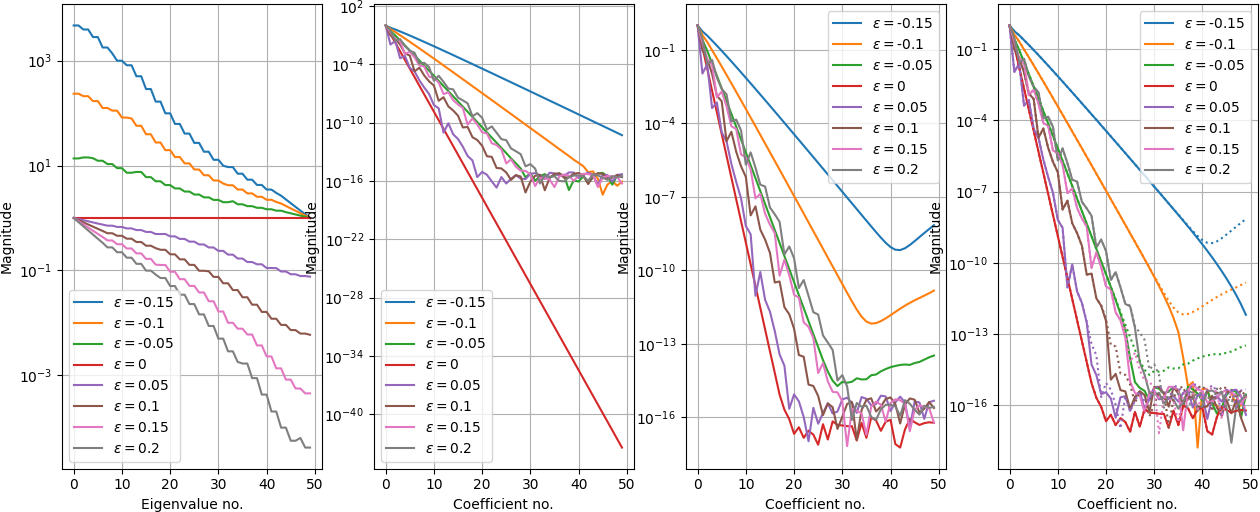
\includegraphics[width=\textwidth]{dat/projection_different_eps.png}
\caption{(a) Eigenvalues of projection operator for different $\varepsilon$; (b) Projection of clean data; (c) Projection of polluted data; (d) Projection of polluted data with small steps and thresholding}
\end{figure}

To inspect the behavior of the projection operator more closely, let us consider projection of a series which coefficients are given by $a_i = \exp\of{-100i}$. The results of projection with different $\varepsilon$ are given in Figure~\ref{fig:projection} (b) and, at the first glance, do not indicate of any instabilities. However, this is likely due to coefficients $a_i$ decaying very fast. Indeed, if we add a random noise to coefficients $a_i$ then the projection results seem to stay stable only if $\varepsilon > 0$ while for $\varepsilon < 0$ high-order coefficients growing uncontrollably (see Figure~\ref{fig:projection} (c)). 

A possible fix could be to use multiple small projection steps with zeroing all coefficients below a chosen threshold after each sub-step. The example of such a strategy is given in  Figure~\ref{fig:projection} (d) where a target relative change $\varepsilon_0 = 0.001$ was used (that is, the number of sub-steps and their size are chosen as $m = \text{ceil}\of{\frac{\log\of{1+\varepsilon}}{\log\of{1+\varepsilon_0}}}$ and $\tilde{\varepsilon} = \sqrt[n]{1+\varepsilon} - 1$). This strategy produces almost identical results as in the case of one full step and does not result in an uncontrollable growth of high-order coefficients for $\varepsilon < 0$. However, it is unclear whether there are any growing instabilities in the low-order part of the spectrum which are not seen due to large values of the coefficients there.


\begin{figure}[H]
\centering
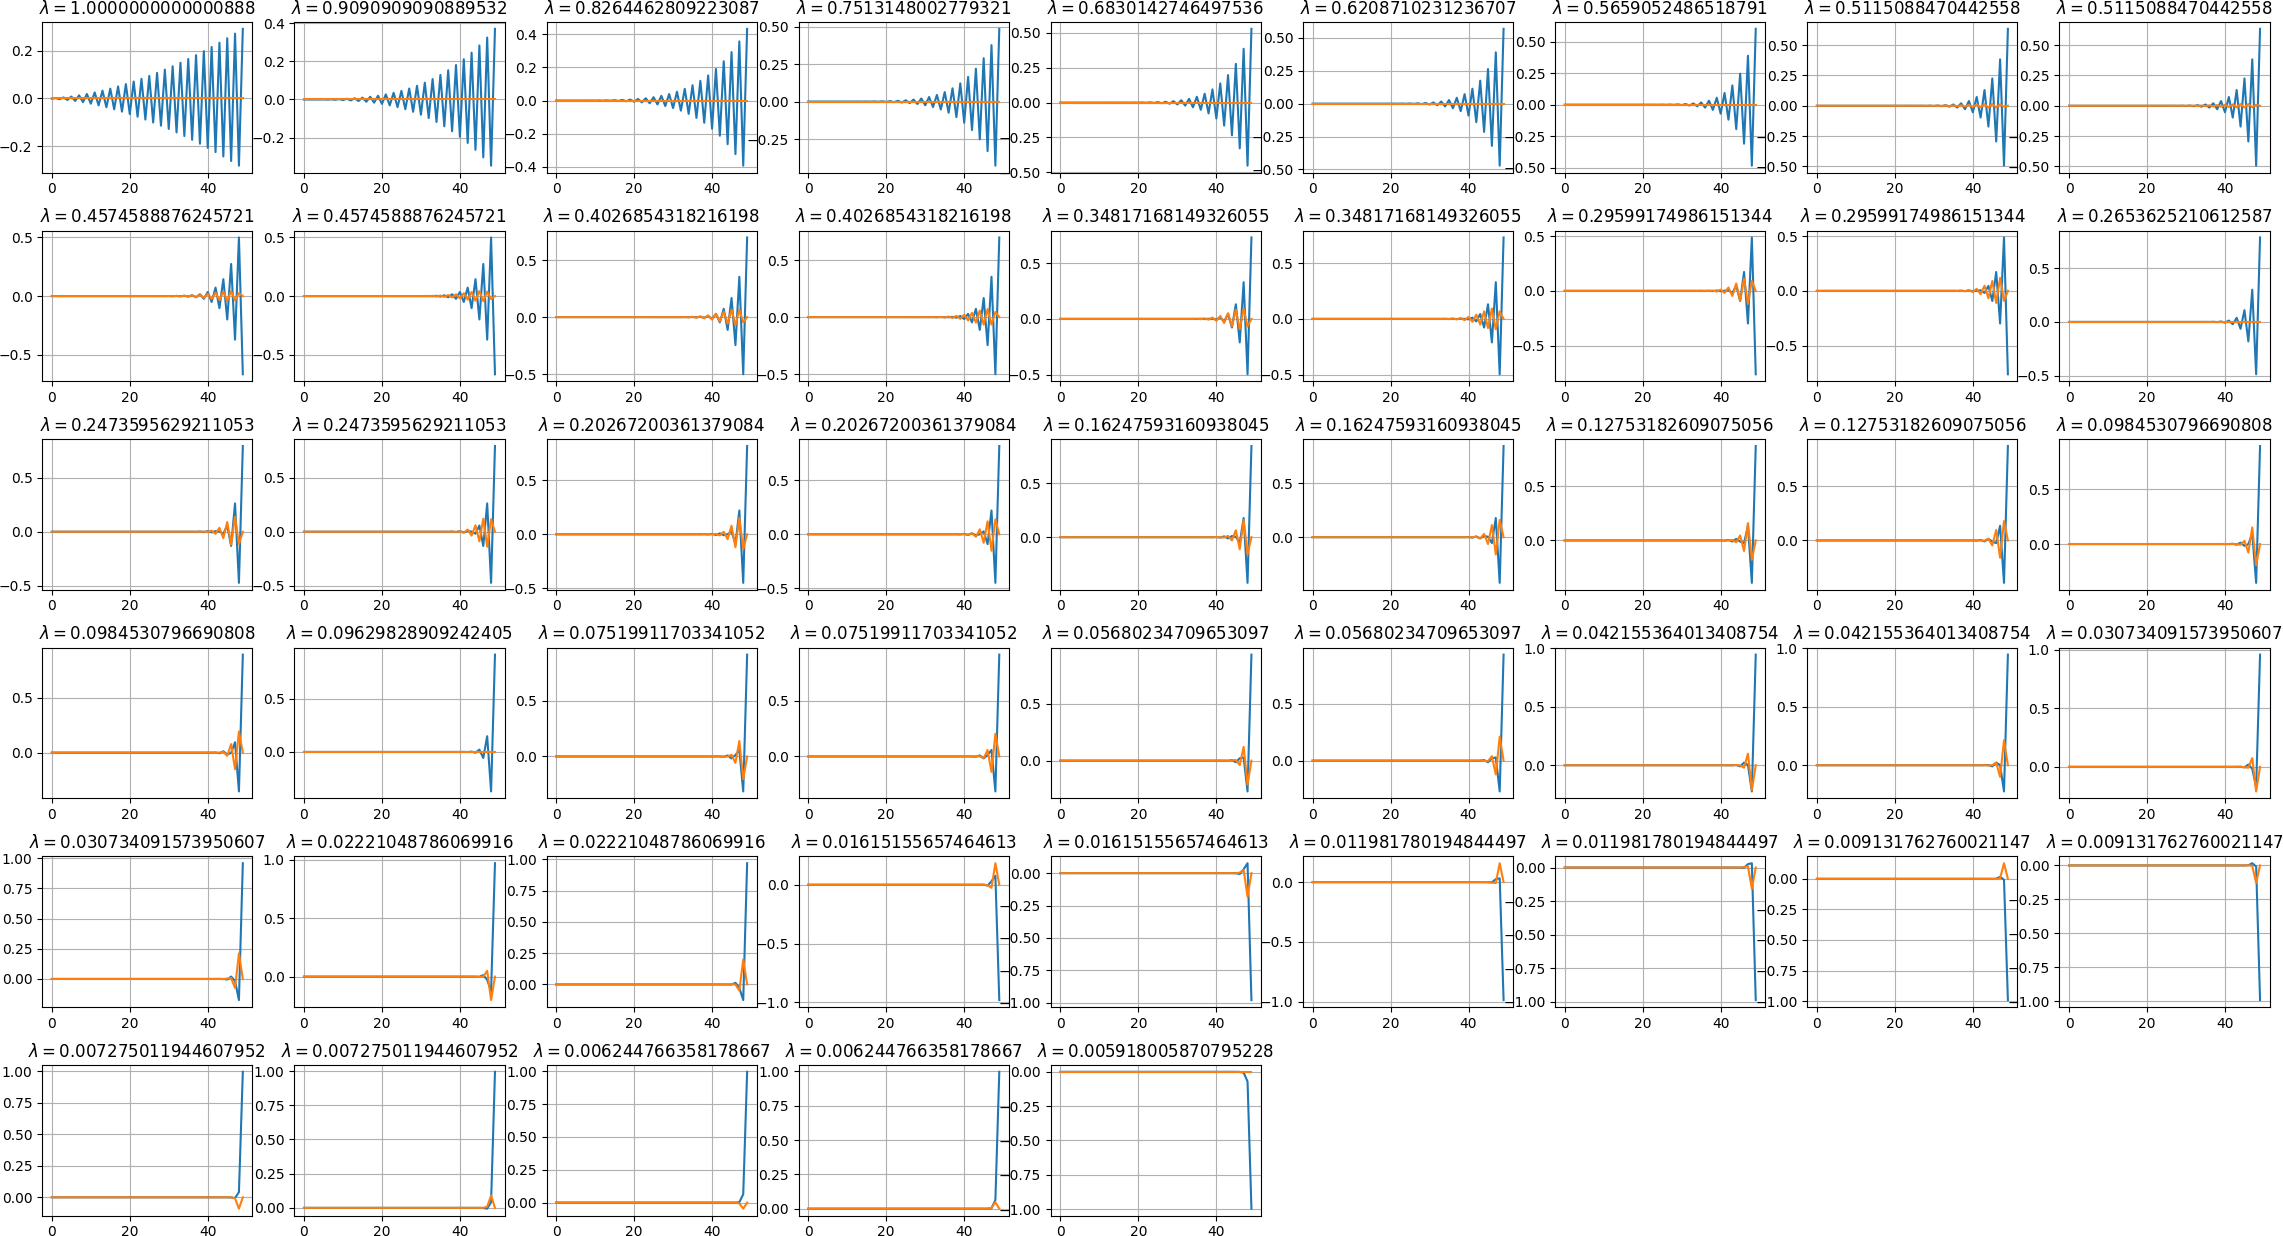
\includegraphics[width=1.2\textwidth]{dat/projection_pos_eigs.png}
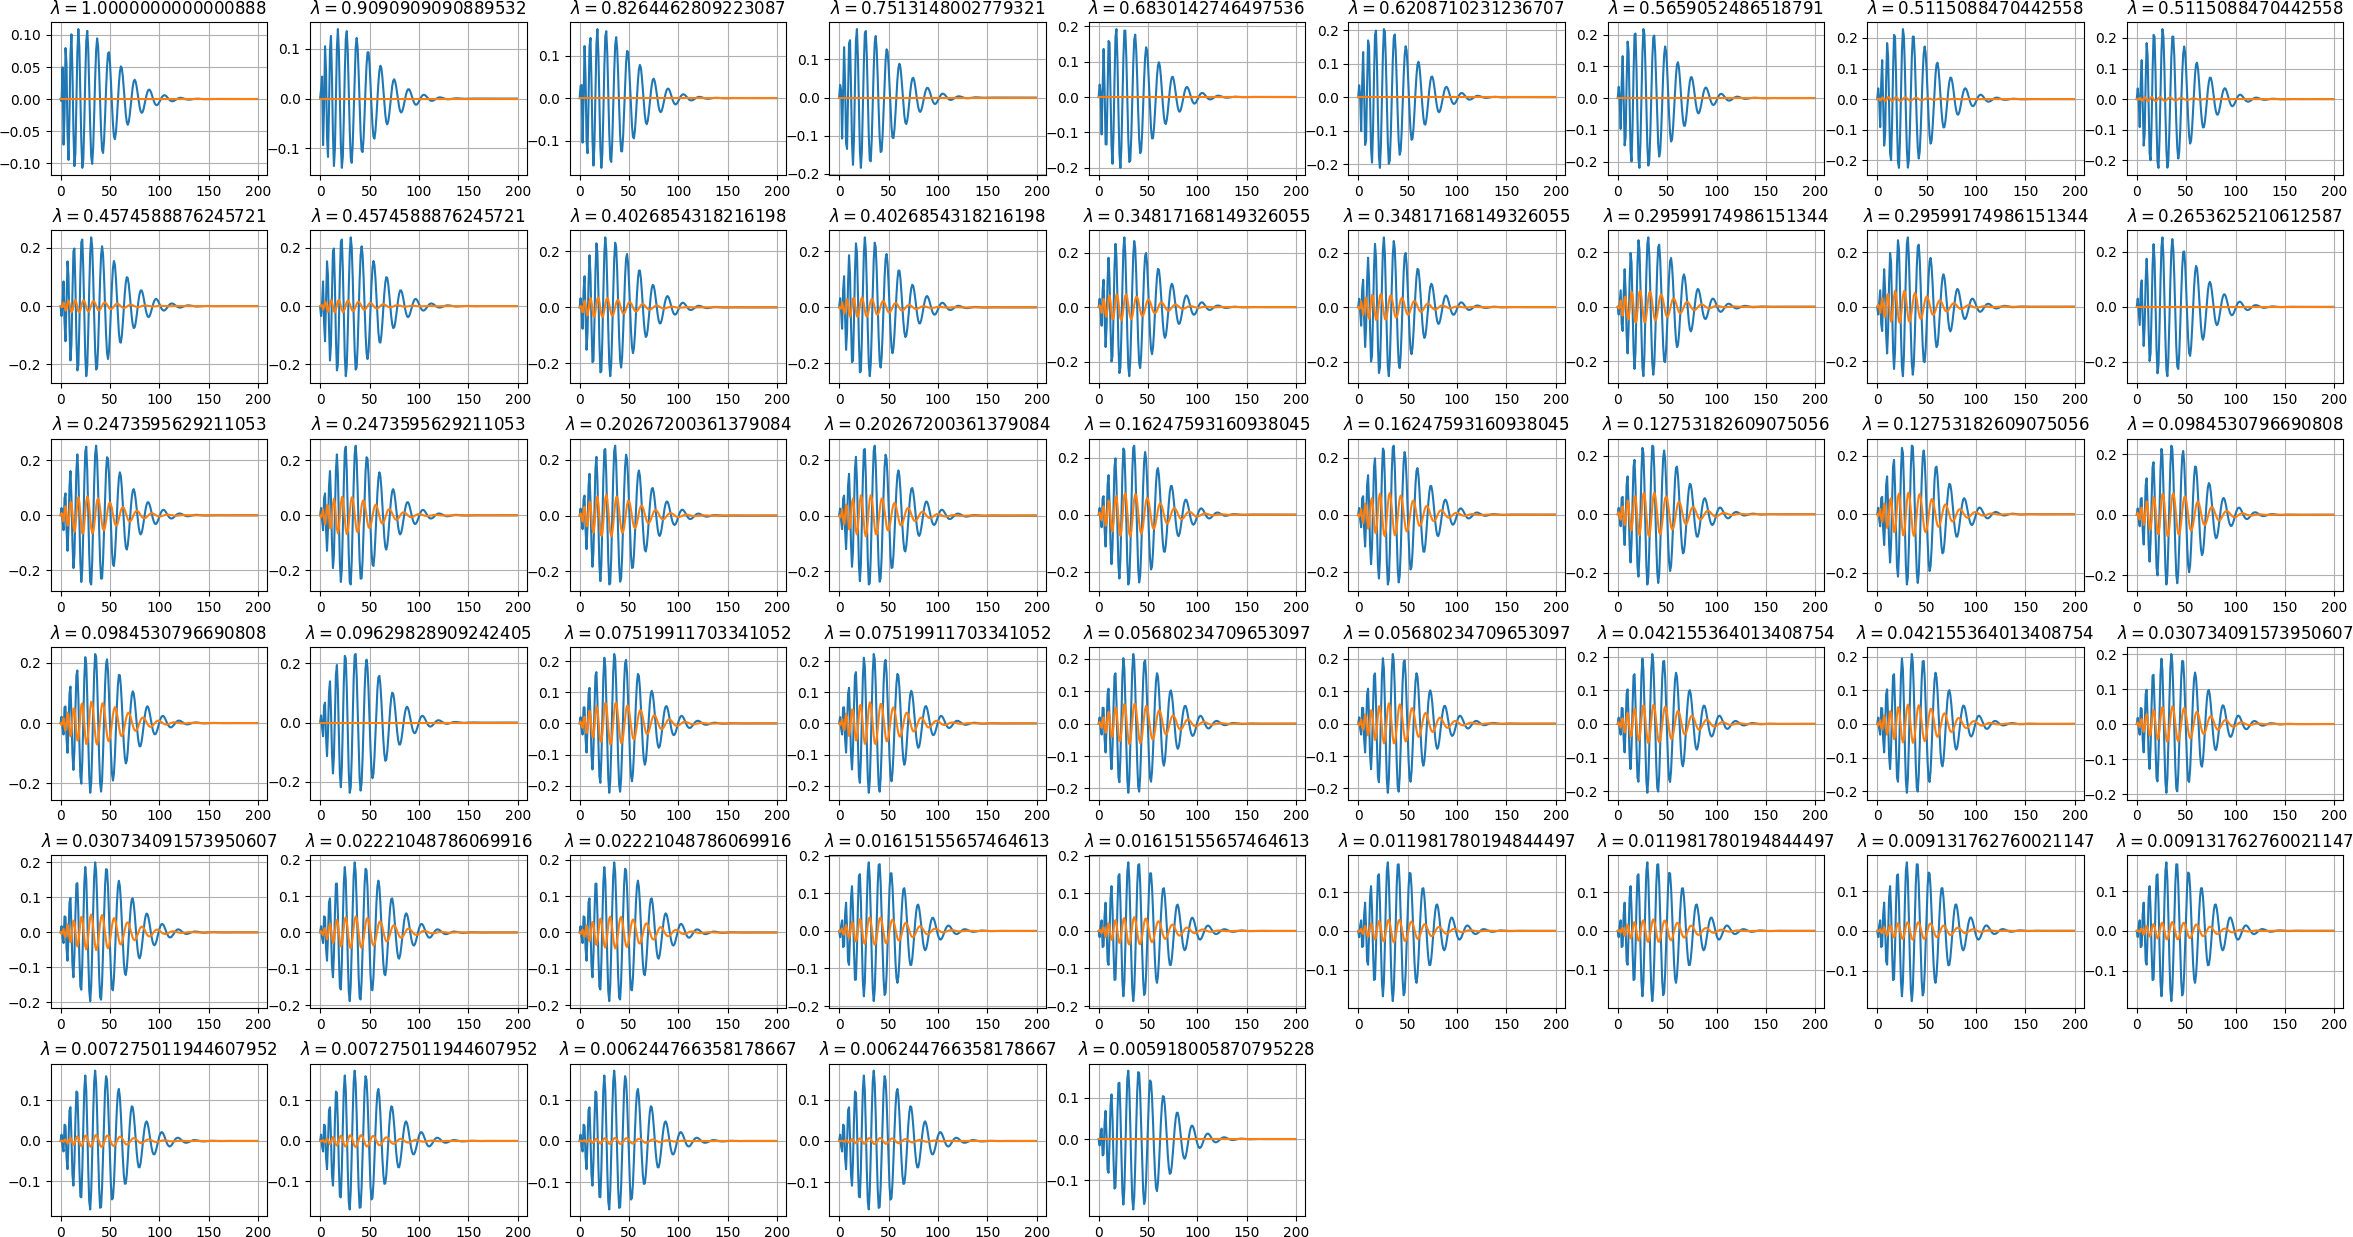
\includegraphics[width=1.2\textwidth]{dat/projection_pos_eigs_visual.png}
\caption{Eigenvectors (top) and their visualization (bottom) for $\varepsilon = 0.1$}
\end{figure}

\begin{figure}[H]
\centering
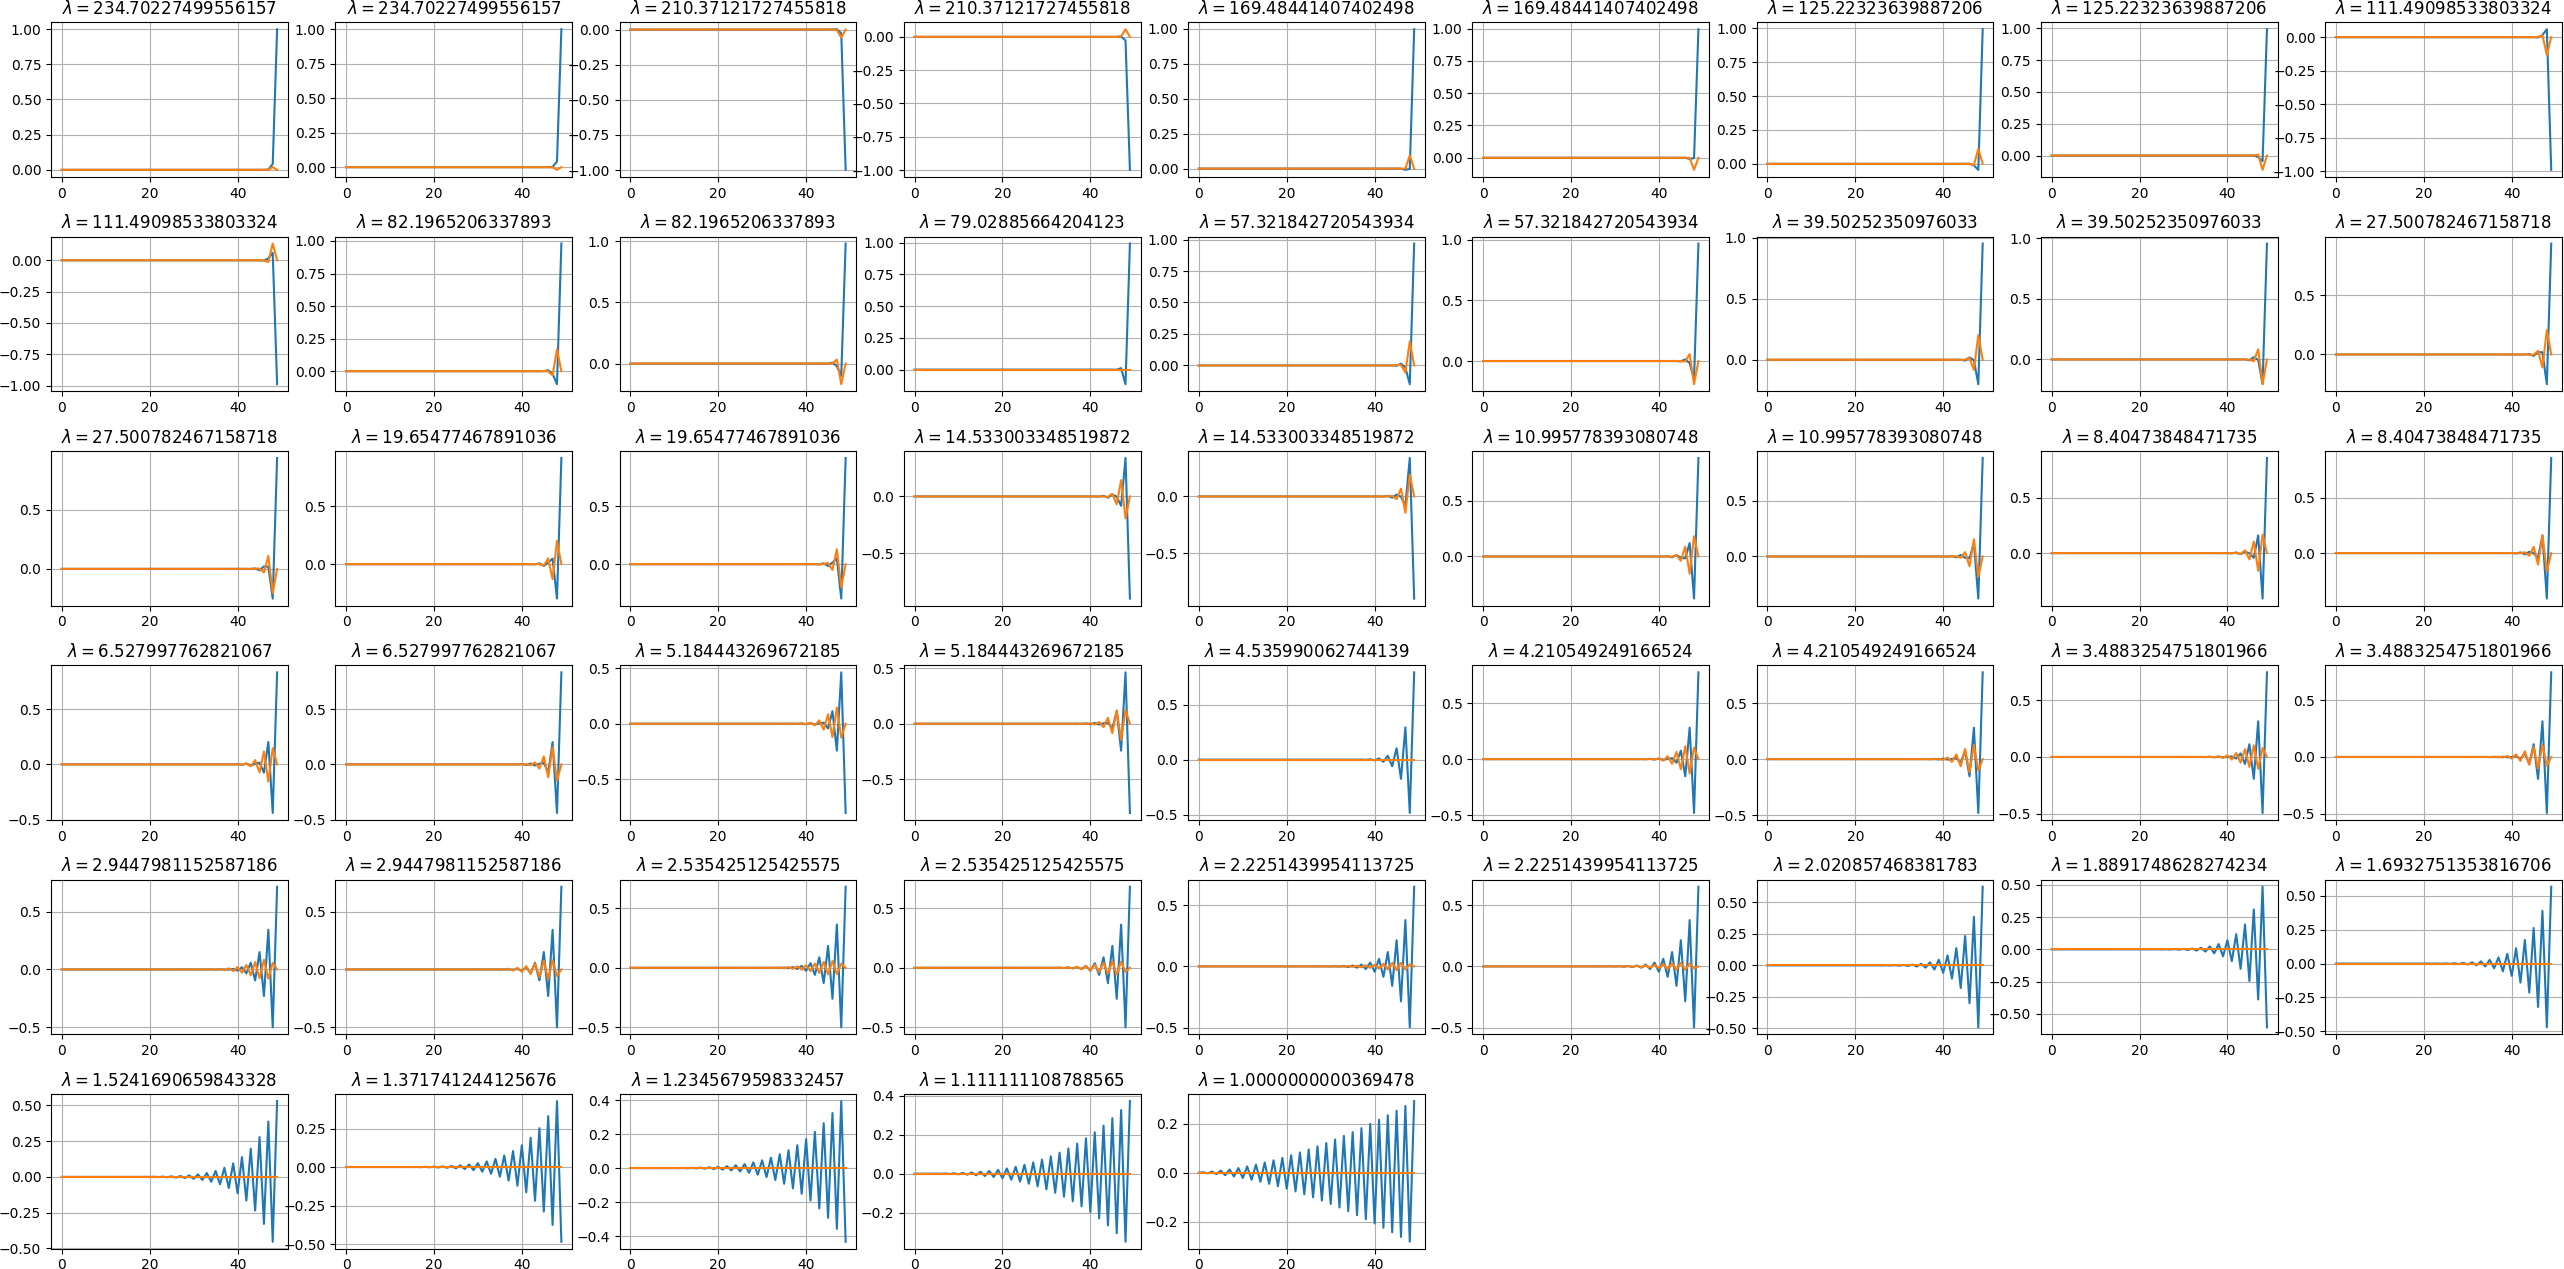
\includegraphics[width=1.2\textwidth]{dat/projection_neg_eigs.png}
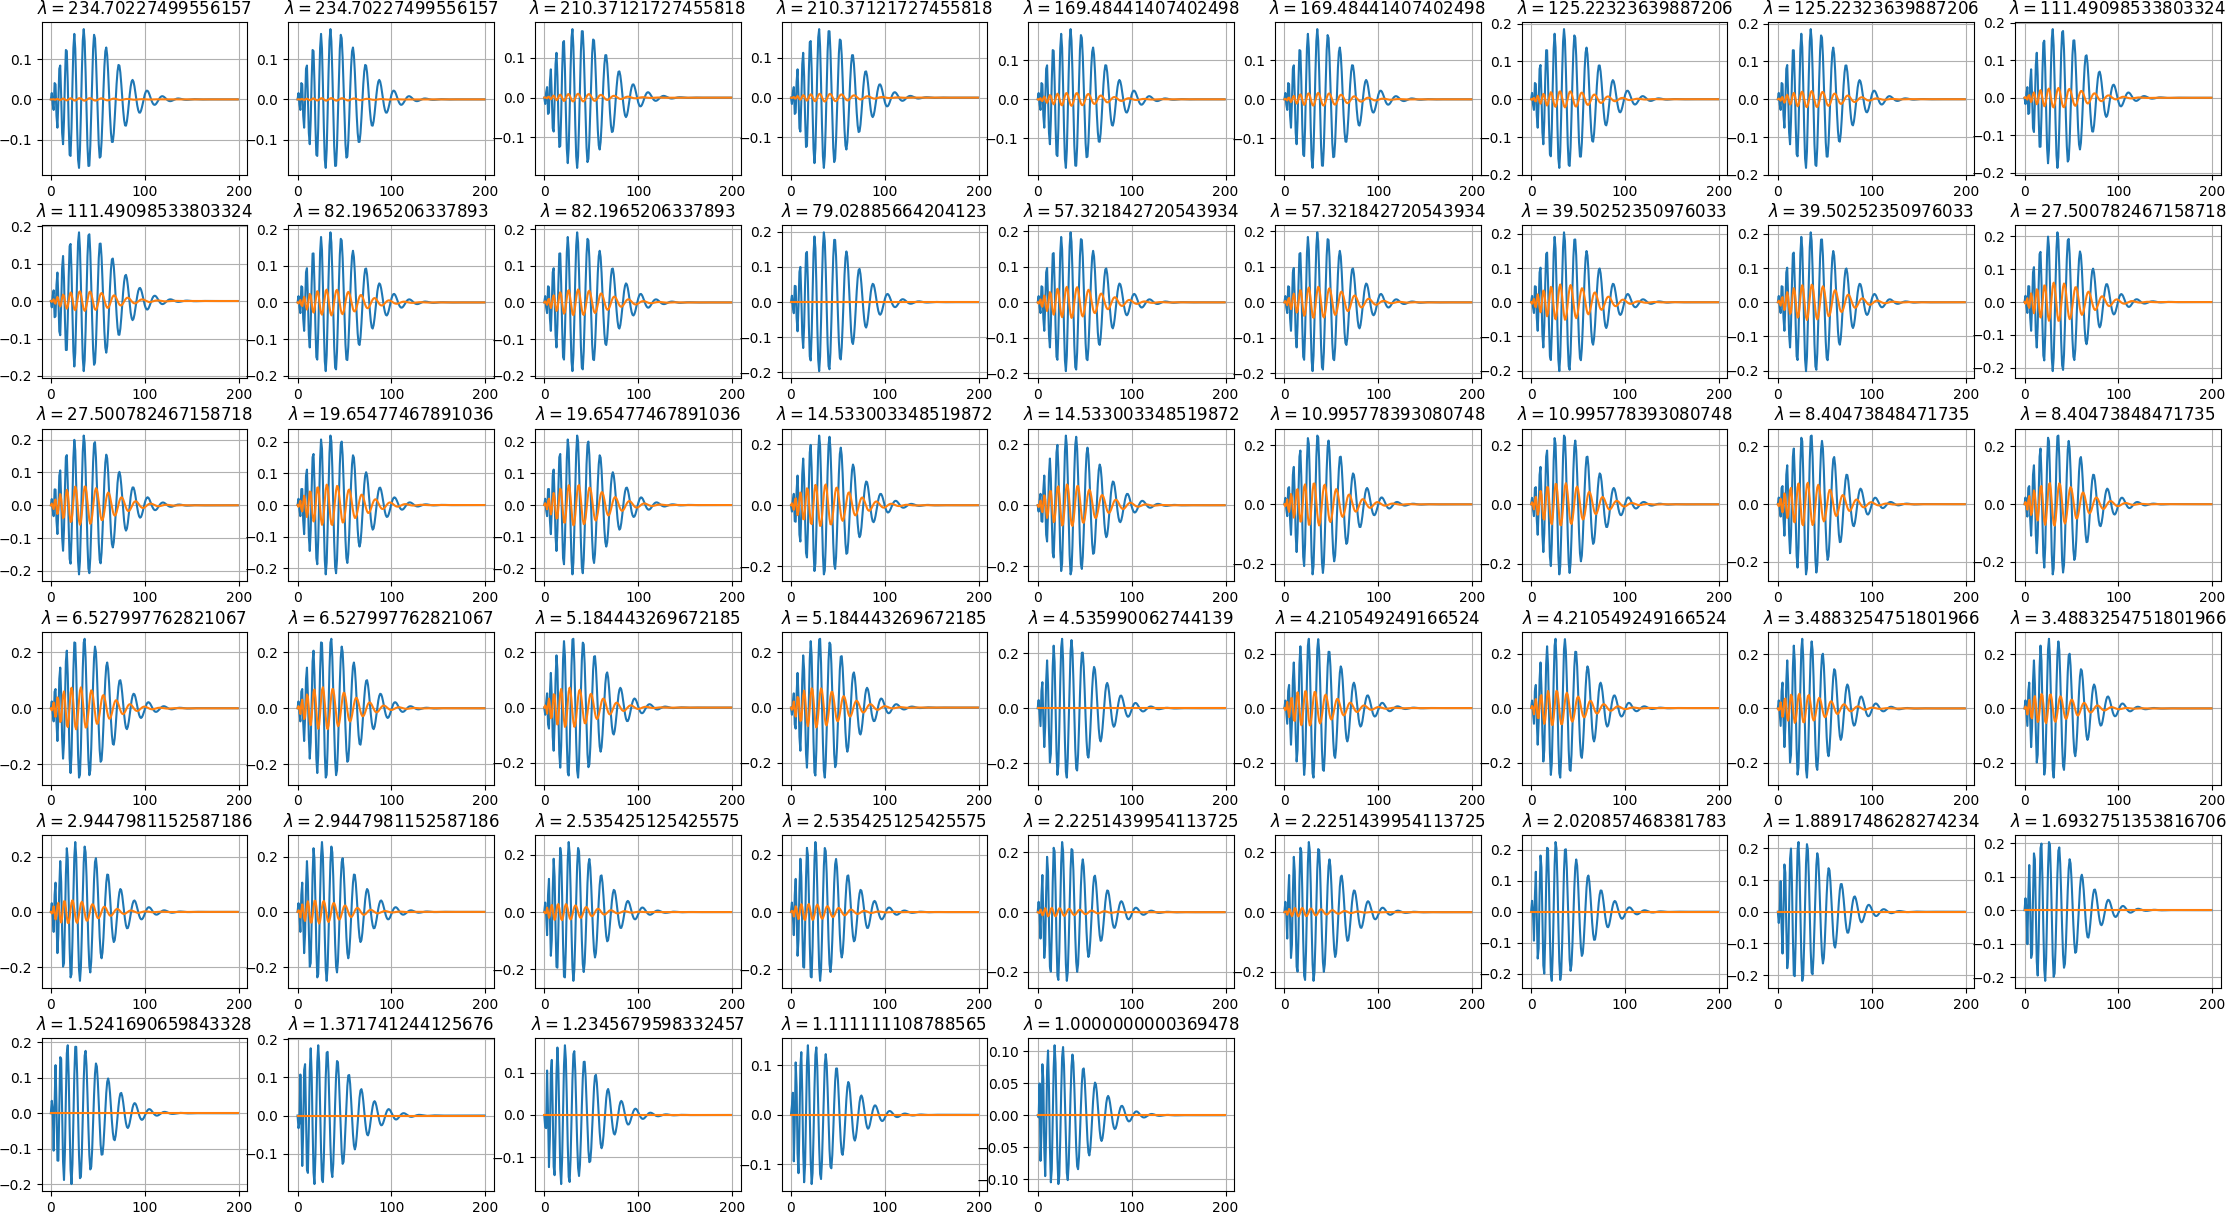
\includegraphics[width=1.2\textwidth]{dat/projection_neg_eigs_visual.png}
\caption{Eigenvectors (top) and their visualization (bottom) for $\varepsilon = -0.1$}
\end{figure}

\clearpage
\section{Advection term (initial poor attempt)}
Advection (acceleration) term
\begin{align*}
\partial_t f + \vect{E}\cdot \nabla_{\vect{v}} f = 0
\end{align*}

In spherical coordinates
\begin{align*}
\nabla_{\vect{v}} 
= \vrunit \frac{\partial}{\partial \vr}
+ \vthetaunit \frac{1}{\vr} \frac{\partial}{\partial \vtheta}
+ \vphiunit \frac{1}{\vr \sin\of{\vtheta}} \frac{\partial}{\partial \vphi}
\end{align*}

\begin{align*}
\vect{E} 
= E \hat{\vect{z}} 
= E \left( \cos\of{\vtheta} \vrunit - \sin\of{\vtheta} \vthetaunit \right)
\end{align*}


\begin{align*}
\vect{E}\cdot \nabla_{\vect{v}} f
= E 
\left( \cos\of{\vtheta} \frac{\partial f}{\partial \vr} 
- \sin\of{\vtheta} \frac{1}{\vr} \frac{\partial f}{\partial \vtheta} \right)
\end{align*}

Expansion in terms of Maxwell polynomials and spherical harmonics
\begin{align*}
f = A 
\exp\of{-\left(\frac{\vr}{\vth}\right)^2} 
\sum_{klm} a_{klm} P_k\of{\textstyle\frac{v}{\vth}} Y_{lm}\of{\vtheta,\vphi}
\end{align*}

Differentiation and lifting matrices
\begin{align*}
P^\prime_k\of{x} &= \sum_{j=0}^{N_r} d_{jk} P_j\of{x}
&
&\rightarrow \quad
\sum_{k=0}^{N_r} a_k P^\prime_k\of{x} 
= \sum_{k=0}^{N_r} \sum_{j=0}^{N_r} d_{jk} a_k P_j\of{x}
= \sum_{j=0}^{N_r} \left( \sum_{k=0}^{N_r} d_{jk} a_k \right) P_j\of{x}
\\
x P_k\of{x} &= \sum_{j=0}^{N_r} l_{jk} P_k\of{x}
&
&\rightarrow \quad
\sum_{k=0}^{N_r} a_k x P_k\of{x} 
= \sum_{k=0}^{N_r} \sum_{j=0}^{N_r} l_{jk} a_k P_j\of{x}
= \sum_{j=0}^{N_r} \left( \sum_{k=0}^{N_r} l_{jk} a_k \right) P_j\of{x}
\end{align*}
where $d_{jk}$ and $l_{jk}$ are calculated from recursive coefficients generating polynomials

\begin{align*}
\left( e^{-x^2} P_k\of{x} \right)^\prime
= - 2 x e^{-x^2} P_k\of{x} + e^{-x^2} P^\prime_k\of{x}
&= e^{-x^2} \sum_{j=0}^{N_r} \left( d_{jk} - 2 l_{jk} \right)P_j\of{x}
\\
&= e^{-x^2} \sum_{j=0}^{N_r} g_{jk} P_j\of{x}
\end{align*}

\begin{align*}
\frac{\partial f}{\partial v}
=
\frac{1}{\vth}
A \exp\of{-\left(\frac{\vr}{\vth}\right)^2} 
\sum_{lm} \sum_{j=0}^{N_r} 
\left(\sum_{k=0}^{N_r} g_{jk} a_{klm} \right) 
P_j\of{\frac{\vr}{\vth}} Y_{lm}\of{\vtheta,\vphi}
\end{align*}

\begin{align*}
\frac{1}{\vr}\frac{\partial f}{\partial \vtheta}
=
\frac{1}{\vr} A \exp\of{-\left(\frac{\vr}{\vth}\right)^2} 
\sum_{klm} a_{klm} P_k\of{\frac{\vr}{\vth}} 
\frac{\partial}{\partial \vtheta} Y_{lm}\of{\vtheta,\vphi}
\end{align*}

\begin{multline*}
\myint \cos\of{\vtheta} \frac{\partial f}{\partial \vr} P_p\of{\frac{\vr}{\vth}} Y_{qs}\of{\vtheta,\vphi} \vr^2 \diff{\vr} \diff{\vomega}
\\
=
\frac{1}{\vth}
A \sum_{lm} \sum_{j=0}^{N_r} \left(\sum_{k=0}^{N_r} g_{jk} a_{klm} \right) 
\left(
\int 
\exp\of{-\left(\frac{\vr}{\vth}\right)^2} P_j\of{\frac{v}{\vth}} P_p\of{\frac{\vr}{\vth}} \vr^2 
\diff{v}
\right)
\\
\times
\left(
\int
\cos\of{\vtheta} 
Y_{lm}\of{\vtheta,\vphi}
Y_{qs}\of{\vtheta,\vphi}
\diff{\vomega}
\right)
\\
=
\vth^2
A \sum_{lm} \sum_{j=0}^{N_r} \left(\sum_{k=0}^{N_r} g_{jk} a_{klm} \right) 
M_{p} \delta_{j,p}
\Psi_{lmqs}
=
\vth^2
A \sum_{lm} \left(\sum_{k=0}^{N_r} g_{pk} a_{klm} \right) 
M_{p}
\Psi_{lmqs}
\end{multline*}

\begin{multline*}
\myint \sin\of{\vtheta} \frac{1}{\vr} \frac{\partial f}{\partial \vtheta} P_p\of{\frac{v}{\vth}} Y_{qs}\of{\vtheta,\vphi} \vr^2 \diff{\vr} \diff{\vomega}
=
\\
A \sum_{lm} \sum_{j=0}^{N_r} \left(\sum_{k=0}^{N_r} g_{jk} a_{klm} \right) 
\left(
\int 
\exp\of{-\left(\frac{\vr}{\vth}\right)^2} P_j\of{\frac{\vr}{\vth}} P_p\of{\frac{\vr}{\vth}} \vr
\diff{\vr}
\right)
\\
\times
\left(
\int
\sin\of{\vtheta} 
Y_{qs}\of{\vtheta,\vphi}
\frac{\partial}{\partial \vtheta}
Y_{lm}\of{\vtheta,\vphi}
\diff{\vomega}
\right)
\end{multline*}

\begin{multline*}
\int 
\exp\of{-\left(\frac{\vr}{\vth}\right)^2} P_j\of{\frac{\vr}{\vth}} P_p\of{\frac{\vr}{\vth}} \vr
\diff{\vr}
=
\vth^2
\int 
e^{-x^2} P_j\of{x} P_p\of{x} x
\diff{x}
\\
=
-
\frac{\vth^2}{2}
\int 
x^2
\left(
e^{-x^2} P_j\of{x} P_p\of{x}
\right)'
\diff{x}
\\
=
-
\frac{\vth^2}{2}
\int 
x^2
e^{-x^2} 
\left(
-2x
P_j\of{x} P_p\of{x}
+
P^\prime_j\of{x} P_p\of{x}
+
P_j\of{x} P^\prime_p\of{x}
\right)
\diff{x}
\\
=
\frac{\vth^2}{2}
\int 
x^2
e^{-x^2} 
\left(
\sum_{k} 2l_{kj} P_k\of{x} P_p\of{x}
-
\sum_{k} d_{kj} P_k\of{x} P_p\of{x}
-
\sum_{k} d_{kp} P_j\of{x} P_k\of{x}
\right)
\diff{x}
\\
=
\frac{\vth^2}{2}
\left(
\sum_{k} 2l_{kj} \int x^2 e^{-x^2} P_k\of{x} P_p\of{x} \diff{x}
-
\sum_{k} d_{kj} \int x^2 e^{-x^2} P_k\of{x} P_p\of{x} \diff{x}
-
\sum_{k} d_{kp} \int x^2 e^{-x^2} P_j\of{x} P_k\of{x} \diff{x}
\right)
\\
=
-
\frac{\vth^2}{2}
\left(
\sum_{k} g_{kj} M_p \delta_{k,p}
+
\sum_{k} d_{kp} M_j \delta_{k,j} 
\right)
=
-
\frac{\vth^2}{2}
\left(
g_{pj} M_p
+
d_{jp} M_j
\right)
\end{multline*}

\begin{multline*}
\myint \sin\of{\vtheta} \frac{1}{\vr} \frac{\partial f}{\partial \vtheta} P_p\of{\textstyle\frac{\vr}{\vth}} Y_{qs}\of{\vtheta,\vphi} \vr^2 \diff{\vr} \diff{\vomega}
=
\\
-
\frac{\vth^2}{2}
A \sum_{lm} \sum_{j=0}^{N_r} \left(\sum_{k=0}^{N_r} g_{jk} a_{klm} \right) 
\left(
g_{pj} M_p
+
d_{jp} M_j
\right)
\Phi_{lmqs}
\end{multline*}

\begin{multline*}
\myint \vect{E}\cdot \nabla_{\vect{v}} f P_p\of{\textstyle\frac{\vr}{\vth}} Y_{qs}\of{\theta,\phi} \vr^2 \diff{\vr} \diff{\vomega}
\\
=
E
\vth^2
A \sum_{lm} \left(\sum_{k=0}^{N_r} g_{pk} a_{klm} \right) 
M_{p}
\Psi_{lmqs}
+
\frac{\vth^2}{2}
A \sum_{lm} \sum_{j=0}^{N_r} \left(\sum_{k=0}^{N_r} g_{jk} a_{klm} \right) 
\left(
g_{pj} M_p
+
d_{jp} M_j
\right)
\Phi_{lmqs}
\\
=
E
\sum_{klm}
\epsilon_{pqsklm} a_{klm}
\end{multline*}

\begin{align*}
\epsilon_{pqsklm} =
\vth^2 A 
\left(
g_{pk} M_{p} \Psi_{lmqs}
+
\frac{1}{2}
\sum_{j=0}^{N_r} g_{jk} 
\left(
g_{pj} M_p
+
d_{jp} M_j
\right)
\Phi_{lmqs}
\right)
\end{align*}


Let the polynomials on the radial direction is defined as, 
\begin{align}
	P_{kl} = b_k(x) x^l
\end{align} where $b_k$ be the $k^{th}$ bspline polynomial. 

For expansion using bspline polynomials in the radial direction we can write, 
\begin{align}
f(\vect{v}) &= \sum_{klm} a_{klm} P_{kl}\of{\textstyle\frac{v}{\vth}} Y_{lm}\of{\vtheta,\vphi}\\
\partial_v f &= \frac{1}{\vth} \sum_{klm} a_{klm} P^\prime_{kl}\of{\textstyle\frac{v}{\vth}} Y_{lm}\of{\vtheta,\vphi}\\
\frac{1}{v}\partial_{v_\theta} f &= \sum_{klm} a_{klm} P_{kl}\of{\textstyle\frac{v}{\vth}} \partial_{v_\theta} Y_{lm}\of{\vtheta,\vphi}
\end{align}

\begin{multline}
\myint \myint \cos\of{\vtheta} \frac{\partial f}{\partial \vr} P_{pq}\of{\frac{\vr}{\vth}} Y_{qs}\of{\vtheta,\vphi} \vr^2 \diff{\vr} \diff{\vomega}= \\
\sum_{klm} a_{klm} \myint \myint \frac{v^2}{\vth}  P^\prime_{kl}\of{\frac{\vr}{\vth}} P_{pq}\of{\frac{\vr}{\vth}} \cos\of{\vtheta} Y_{lm}\of{\vtheta,\vphi} Y_{qs}\of{\vtheta,\vphi} \diff{v}\diff{v_\omega} =\\
\sum_{klm} a_{klm} \myint \frac{v^2}{\vth}  P^\prime_{kl}\of{\frac{\vr}{\vth}} P_{pq}\of{\frac{\vr}{\vth}} \diff{v} \Psi_{lmqs}
\end{multline}

\begin{multline*}
\myint \myint \sin\of{\vtheta} \frac{1}{\vr} \frac{\partial f}{\partial \vtheta} P_{pq}\of{\textstyle\frac{\vr}{\vth}} Y_{qs}\of{\vtheta,\vphi} \vr^2 \diff{\vr} \diff{\vomega} = \\
\sin\of{\vtheta}\left(\sum_{klm} a_{klm} P_{kl}\of{\textstyle\frac{v}{\vth}} \partial_{v_\theta} Y_{lm}\of{\vtheta,\vphi} \right) P_{pq}\of{\textstyle\frac{\vr}{\vth}} Y_{qs}\of{\vtheta,\vphi} \vr \diff{\vr} \diff{\vomega} = \\
\sum_{klm} a_{klm} \myint v P_{pq}\of{\textstyle\frac{v}{\vth}} P_{kl}\of{\textstyle\frac{v}{\vth}} dv \myint \sin\of{\vtheta} \partial_{v_\theta} Y_{lm}\of{\vtheta,\vphi}  Y_{qs}\of{\vtheta,\vphi} \diff{v_{\omega}} = \\
\sum_{klm} a_{klm} \myint v P_{pq}\of{\textstyle\frac{v}{\vth}} P_{kl}\of{\textstyle\frac{v}{\vth}} dv \phi_{lmqs}
\end{multline*}


\subsection{Case of Laguerre polynomials (fancy attempt)}
An attempt to compute advection operator analytically in the case of Laguerre polynomials. There are some mistakes early on that propagates throughout the derivations. However, it still gives an overall idea how to proceed. Maybe will revisit later.

\begin{align*}
\lp{l}{0}\of{x} &= 1 \\
\lp{l}{1}\of{x} &= 1 + l - x \\
\lp{l}{k+1}\of{x} &= \frac{(2k+1+l-x) \lp{l}{k}\of{x} - (k+l) \lp{l}{k-1}\of{x}}{k+1}
\end{align*}

\begin{align*}
\myint_0^\infty e^{-x} x^l \lp{l}{k}\of{x} \lp{l}{p}\of{x} \diff{x} = \frac{\Gamma\of{p + l + 1}}{n!} \delta_{k,p}
\end{align*}

\begin{align*}
\lph{l}{k} = \lp{l+1/2}{k}
\end{align*}

\begin{align*}
\Phi_{kl}\of{x} &= e^{-x^2} x^l \lph{l}{k}\of{x^2} \\
\Psi_{pq}\of{x} &= x^q \lph{q}{p}\of{x^2} 
\end{align*}

\begin{align*}
\myint_0^\infty \Phi_{kq}\of{x} \Psi_{pq}\of{x} x^2 \diff{x} 
&= \myint_0^\infty e^{-x^2} x^{2q+2}\lph{q}{k}\of{x^2} \lph{q}{p}\of{x^2} \diff{x}
\\
&= \frac12 \myint_0^\infty e^{-y} y^{q+1/2}\lph{q}{k}\of{y} \lph{q}{p}\of{y} \diff{x}
\\
&= N_{p,q} \delta_{k,p}
\end{align*}

Useful formulae
\begin{align*}
\lph{l+1}{k} \of{x^2} &= \sum_{j=0}^{k} \lph{l}{j}\of{x^2}
\\
\lph{l}{k} \of{x^2} &= \lph{l+1}{k} \of{x^2} - \lph{l+1}{k-1} \of{x^2}
\\
x^2 \lph{l+1}{k} \of{x^2} 
&= (k+l+3/2) \lph{l}{k}\of{x^2} - (k+1) \lph{l}{k+1}\of{x^2}
\\
%x^2 L^{(l+2)}_k \of{x^2} 
%&= (k+l+2) \lp{l+1}{k}\of{x^2} - (k+1) \lp{l+1}{k+1}\of{x^2}
%\\
%&= (k+l+2) \sum_{j=0}^{k} \lp{l}{j}\of{x^2} - (k+1) \sum_{j=0}^{k+1} \lp{l}{j}\of{x^2}
%\\
%&= (l+1) \sum_{j=0}^{k} \lp{l}{j}\of{x^2} - (k+1) \lp{l}{k+1}\of{x^2}
%\\
\frac{d}{dx^2} \lph{l}{k} \of{x^2} &= - \lph{l+1}{k-1} \of{x^2}
\\
\frac{d}{dx} \lph{l}{k} \of{x^2} 
&= 2 x \frac{d}{dx^2} \lph{l}{k}\of{x^2} = - 2 x \lph{l+1}{k-1}\of{x^2}
%\\
%x \frac{d}{dx} \lp{l+1}{k} \of{x^2} 
%&= 2 x^2 \frac{d}{dx^2} \lp{l+1}{k}\of{x^2} = - 2 x^2 \lp{l+2}{k-1}\of{x^2}
%\\
%&= -2(l+1) \sum_{j=0}^{k-1} \lp{l}{j}\of{x^2} 
%+ 2 k \lp{l}{k}\of{x^2}
\end{align*}

%\begin{align*}
%\frac{d}{dx}\Phi_{k,q+1}\of{x} 
%&= - 2 e^{-x^2} x^{q+2} L^{(q+1)}_k\of{x^2}
%+ (q+1) e^{-x^2} x^{q} L^{(q+1)}_k\of{x^2}
%+ e^{-x^2} x^{q+1} \frac{d}{dx} L^{(q+1)}_k\of{x^2}
%\\
%&= e^{-x^2} x^{q} \Big( 
%- 2 (k+q+1) L^{(q)}_k\of{x^2} + 2 (k+1) L^{(q)}_{k+1}\of{x^2} 
%\\&
%+ (q+1) \sum_{j=0}^{k} L^{(q)}_j\of{x^2}
%- 2(q+1) \sum_{j=0}^{k-1} \lp{q}{j}\of{x^2} 
%+ 2 k \lp{q}{k}\of{x^2}
%\Big)
%\\
%&= e^{-x^2} x^{q} \Big( 
%2 (k+1) L^{(q)}_{k+1}\of{x^2} 
%- (q+1) \sum_{j=0}^{k} \lp{q}{j}\of{x^2} 
%\Big)
%\\
%&= 2 (k+1) \Phi_{k+1,q}\of{x}
%- (q+1) \sum_{j=0}^{k} \Phi_{j,q}\of{x} 
%\end{align*}

%\begin{align*}
%\myint_0^\infty \Psi_{p,q}\of{x} \frac{d}{dx}\Phi_{k,q+1}\of{x}  x^2 \diff{x}
%&= 2 (k+1) N_{p,q} \delta_{p,k+1}  - (q+1) \sum_{j=0}^{k} N_{p,q} \delta_{p,j} 
%\\
%&= N_{p,q} \sum_{j=0}^{k+1} \Omega \delta_{p,j} 
%\end{align*}

\begin{multline*}
\tfun{q}{p}\of{x} \frac{d}{dx} \bfun{q+1}{k}\of{x} 
= x^q \lph{q}{p} \frac{d}{dx} e^{-x^2} x^{q+1} \lph{q+1}{k}
\\
= x^q \lph{q}{p} \left( 
- 2 e^{-x^2} x^{q+2} \lph{q+1}{k}\of{x^2}
+ (q+1) e^{-x^2} x^{q} \lph{q+1}{k}\of{x^2}
- 2 e^{-x^2} x^{q+2} \lph{q+2}{k-1}\of{x^2}
\right)
\\ 
= 
-2 x^q \lph{q}{p} e^{-x^2} x^q \left( (k+q+3/2) \lph{q}{k} - (k+1) \lph{q}{k+1} \right) 
\\
+ (q+1) x^q \lph{q}{p} e^{-x^2} x^q \sum_{j=0}^{k} \lph{q}{j}
-2 x^{q+1} \left( \lph{q+1}{p} - \lph{q+1}{p-1} \right) e^{-x^2} x^{q+1} \sum_{j=0}^{k-1} \lph{q+1}{j}
\\ 
= 
-2 \tfun{q}{p} \left( (k+q+3/2) \bfun{q}{k} - (k+1) \bfun{q}{k+1} \right) 
+ (q+1)\tfun{q}{p} \sum_{j=0}^{k} \bfun{q}{j}
-2\left( \tfun{q+1}{p} - \tfun{q+1}{p-1} \right) \sum_{j=0}^{k-1} \bfun{q+1}{j}
\end{multline*}


\begin{multline*}
\myint_0^\infty \tfun{q}{p}\of{x} \frac{d}{dx} \bfun{q+1}{k}\of{x} 
= 
-2 \nfun{q}{p} \left( (k+q+3/2)\delta_{p,k} - (k+1) \delta_{p,k+1} \right) 
+ (q+1)\nfun{q}{p} \sum_{j=0}^{k} \delta_{p,j}
\\
-2\left( \nfun{q+1}{p} \sum_{j=0}^{k-1} \delta_{p,j} - \nfun{q+1}{p-1} \sum_{j=0}^{k-1} \delta_{p-1,j} \right)  
\end{multline*}

Warning: what's below is not correct (forgot 1/2 in Laguerre index)
\begin{align*}
\Phi_{k,q+1}\of{x} \frac{d}{dx}\Psi_{p,q}\of{x} 
&= 
e^{-x^2} x^{q+1} L^{(q+1)}_k\of{x^2}
\left(
q x^{q-1} L^{(q)}_p\of{x^2}
+ x^{q} \frac{d}{dx} L^{(q)}_p\of{x^2}
\right)
\\
&= e^{-x^2} x^{q} \sum_{j=0}^{k} \lp{q}{j}\of{x^2} q x^{q} L^{(q)}_p\of{x^2}
- \Phi_{k,q+1}\of{x} 2 x^{q+1} L^{(q+1)}_{p-1}\of{x^2}
\\
&= q \sum_{j=0}^{k} \Phi_{j,q}\of{x} \Psi_{p,q}\of{x}
- 2\Phi_{k,q+1}\of{x} \Psi_{p-1,q+1}\of{x}
\end{align*}

\begin{align*}
\myint_0^\infty \Phi_{k,q+1}\of{x} \frac{d}{dx}\Psi_{p,q}\of{x} x^2 \diff{x}
&= q \sum_{j=0}^{k} N_{p,q} \delta_{p,j} 
- 2 N_{p,q+1} \delta_{p-1,k} 
\\
&= q \sum_{j=0}^{k} N_{p,q} \delta_{p,j} 
- 2 N_{p,q+1} \delta_{p,k+1} 
\end{align*}

\begin{align*}
\Phi_{k, q-1}\of{x} \frac{d}{dx}\Psi_{pq}\of{x}
&= e^{-x^2} x^{q-1} \lp{q-1}{k}\of{x^2} \frac{d}{dx} x^{q} \lp{q}{p}\of{x^2}
\\
&= e^{-x^2} x^{q-1} \lp{q-1}{k}\of{x^2} 
\left(
q x^{q-1} L^{(q)}_p\of{x^2}
+ x^{q} \frac{d}{dx} L^{(q)}_p\of{x^2}
\right)
\\
&= q \Phi_{k, q-1}\of{x} \sum_{j=0}^p \Psi_{j,q-1}\of{x}
- 2 e^{-x^2} x^{q-1} \lp{q-1}{k}\of{x^2}  x^{q+1} \lp{q+1}{p-1}\of{x^2}
\\
&= q \Phi_{k, q-1}\of{x} \sum_{j=0}^p \Psi_{j,q-1}\of{x}
- 2 e^{-x^2} x^{q} \left( \lp{q}{k}\of{x^2} - \lp{q}{k-1}\of{x^2}\right)  x^{q} \sum_{j=0}^{p-1}\lp{q}{j}\of{x^2}
\\
&= q \sum_{j=0}^p \Phi_{k, q-1}\of{x} \Psi_{j,q-1}\of{x}
- 2 \sum_{j=0}^{p-1} \left( \Phi_{k,q}\of{x^2} - \Phi_{k-1,q}\of{x^2}\right) \Psi_{j,q}\of{x^2}
\end{align*}

\begin{align*}
\myint_0^\infty \Phi_{k, q-1}\of{x} \frac{d}{dx}\Psi_{pq}\of{x} x^2 \diff{x}
&= q \sum_{j=0}^{p} N_{k,q-1} \delta_{k,j} 
- 2 \sum_{j=0}^{p-1} \left( N_{k,q} \delta_{k,j} - N_{k-1,q} \delta_{k-1,j}  \right)
\end{align*}

%\begin{multline*}
%\Psi_{pq}\of{x} \frac{d}{dx}\Phi_{k, q-1}\of{x} 
%= x^q \lp{q}{p}\of{x^2} \frac{d}{dx} e^{-x^2} x^{q-1} \lp{q-1}{k}\of{x^2}
%\\
%= x^q \lp{q}{p}\of{x^2} \left(
%- 2 e^{-x^2} x^{q} L^{(q-1)}_k\of{x^2}
%+ (q-1) e^{-x^2} x^{q-2} L^{(q-1)}_k\of{x^2}
%+ e^{-x^2} x^{q+1} \frac{d}{dx} L^{(q+1)}_k\of{x^2}
%\right)
%\\
%= - x^{q-1} \left( (p+q) \lp{q-1}{p} - (p+1) \lp{q-1}{p+1} \right)
%e^{-x^2} x^{q-1} L^{(q-1)}_k
%\\
%+ (q-1) x^{q-1} \sum_{j=0}^{p} \lp{q-1}{j} e^{-x^2} x^{q-1} \lp{q-1}{k} 
%- 2 x^q \lp{q}{p} e^{-x^2} x^q \lp{q}{k-1}
%\\
%= - (p+q) \tfun{q-1}{p} \bfun{q-1}{k} 
%+ (p+1) \tfun{q-1}{p+1} \bfun{q-1}{k}
%+ (q-1) \sum_{j=0}^{p} \tfun{q-1}{j} \bfun{q-1}{k} 
%- 2 \tfun{q}{p} \bfun{q}{k-1}
%\end{multline*}


\begin{multline*}
\Psi_{pq}\of{x} \frac{d}{dx}\Phi_{k, q-1}\of{x} 
= x^q \lp{q}{p}\of{x^2} \frac{d}{dx} e^{-x^2} x^{q-1} \lp{q-1}{k}\of{x^2}
\\
= x^q \lp{q}{p}\of{x^2} \left(
- 2 e^{-x^2} x^{q} L^{(q-1)}_k\of{x^2}
+ (q-1) e^{-x^2} x^{q-2} L^{(q-1)}_k\of{x^2}
+ e^{-x^2} x^{q+1} \frac{d}{dx} L^{(q+1)}_k\of{x^2}
\right)
\\
= - x^{q} \lp{q}{p} 
e^{-x^2} x^{q} \left( \lp{q}{k} - \lp{q}{k-1} \right)
+ (q-1) x^{q-1} \sum_{j=0}^{p} \lp{q-1}{j} e^{-x^2} x^{q-1} \lp{q-1}{k} 
- 2 x^q \lp{q}{p} e^{-x^2} x^q \lp{q}{k-1}
\\
= - \tfun{q}{p} \bfun{q}{k} 
+ \tfun{q}{p} \bfun{q}{k-1}
+ (q-1) \sum_{j=0}^{p} \tfun{q-1}{j} \bfun{q-1}{k} 
- 2 \tfun{q}{p} \bfun{q}{k-1}
\end{multline*}

\begin{multline*}
\myint_0^\infty \Psi_{pq}\of{x} \frac{d}{dx}\Phi_{k, q-1}\of{x} x^2 \diff{x}
= -  \nfun{q}{p} \delta_{p,k} 
- \nfun{q}{p} \delta_{p,k-1}
+ (q-1) \sum_{j=0}^{p} \nfun{q-1}{j} \delta_{j,k}
\end{multline*}

\newpage
Constant cross-section $t_{end} = 10^{-6}$ s\\
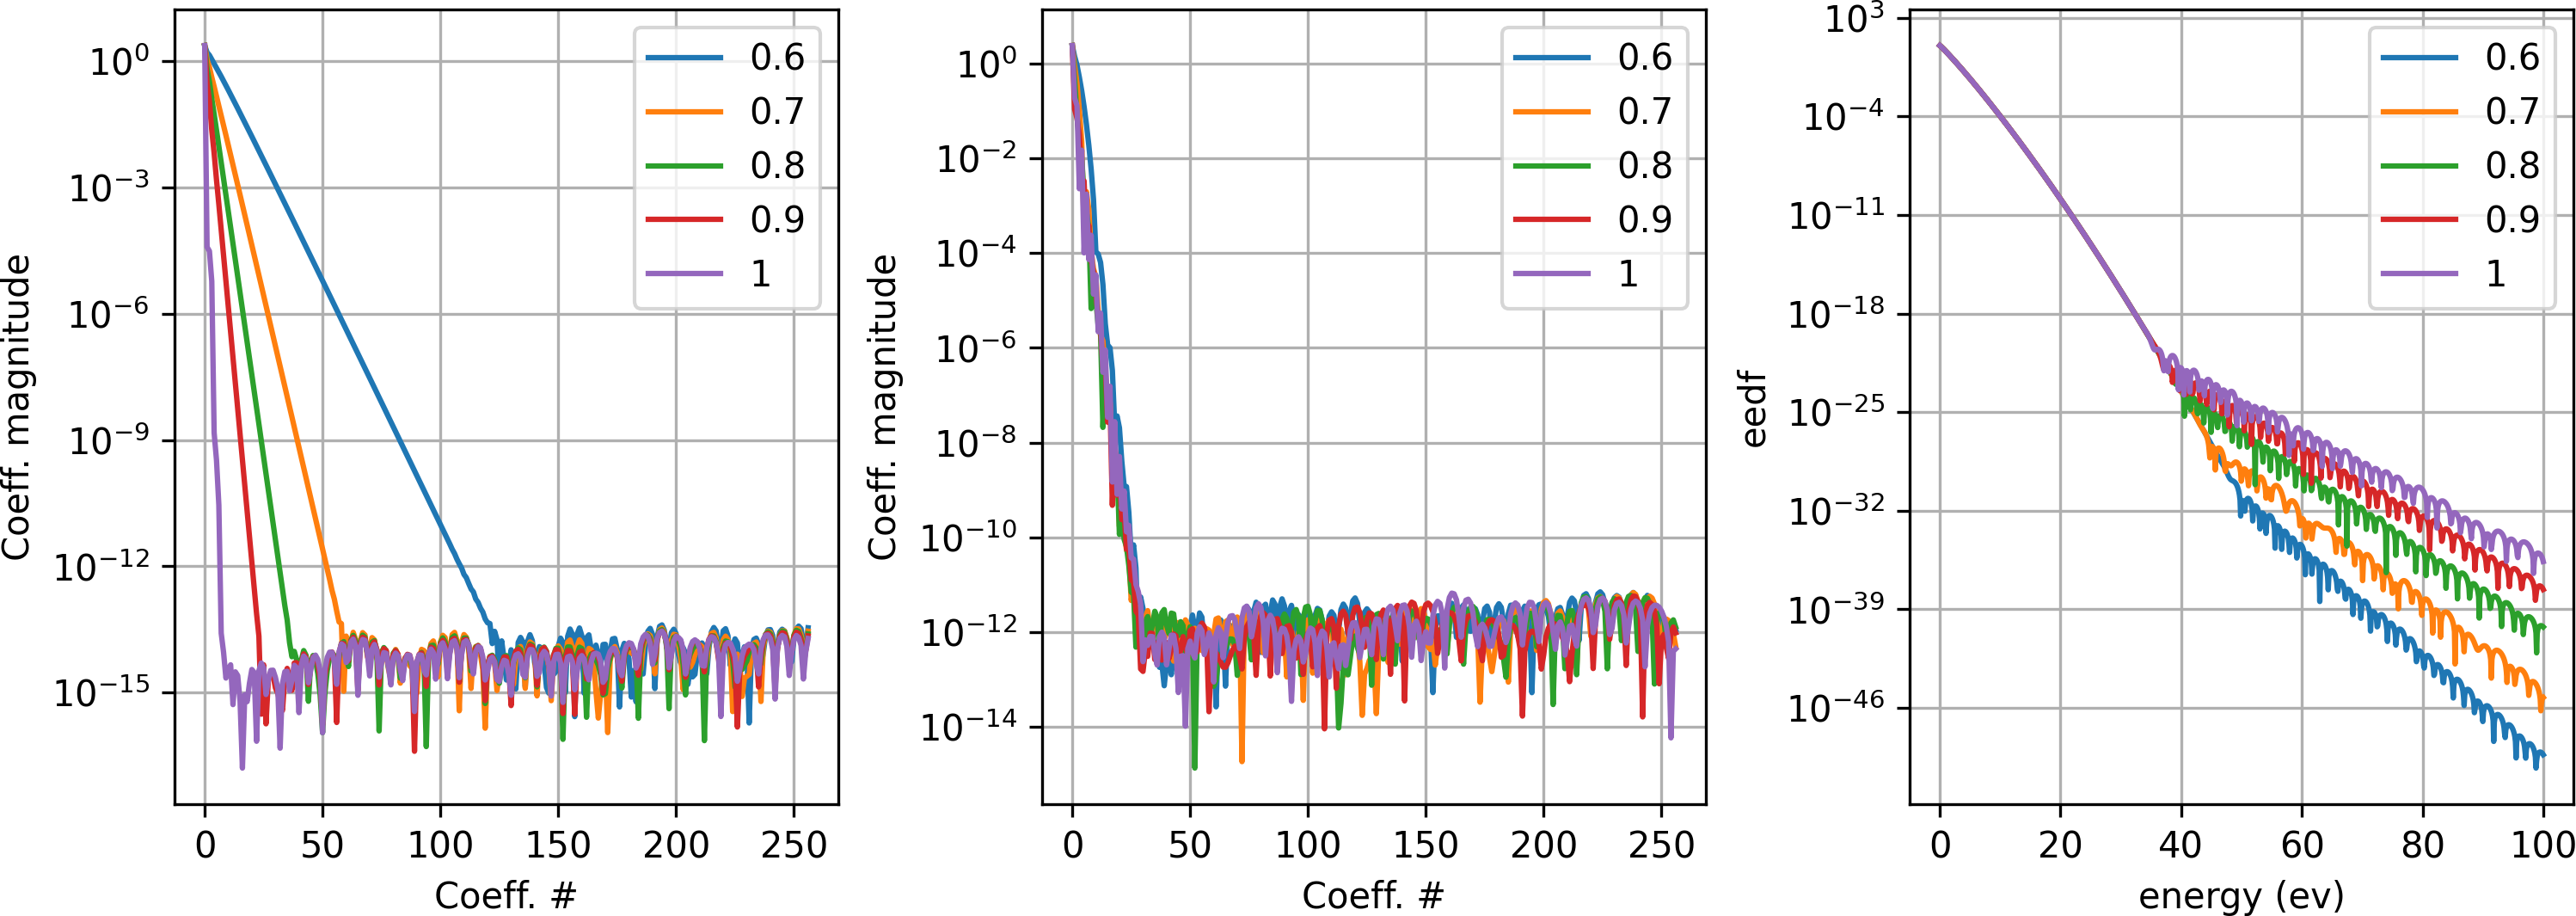
\includegraphics[width=0.99\textwidth]{fig/different_vth_const_1e-6.png}

Data-fitted cross section $t_{end} = 10^{-6}$ s\\
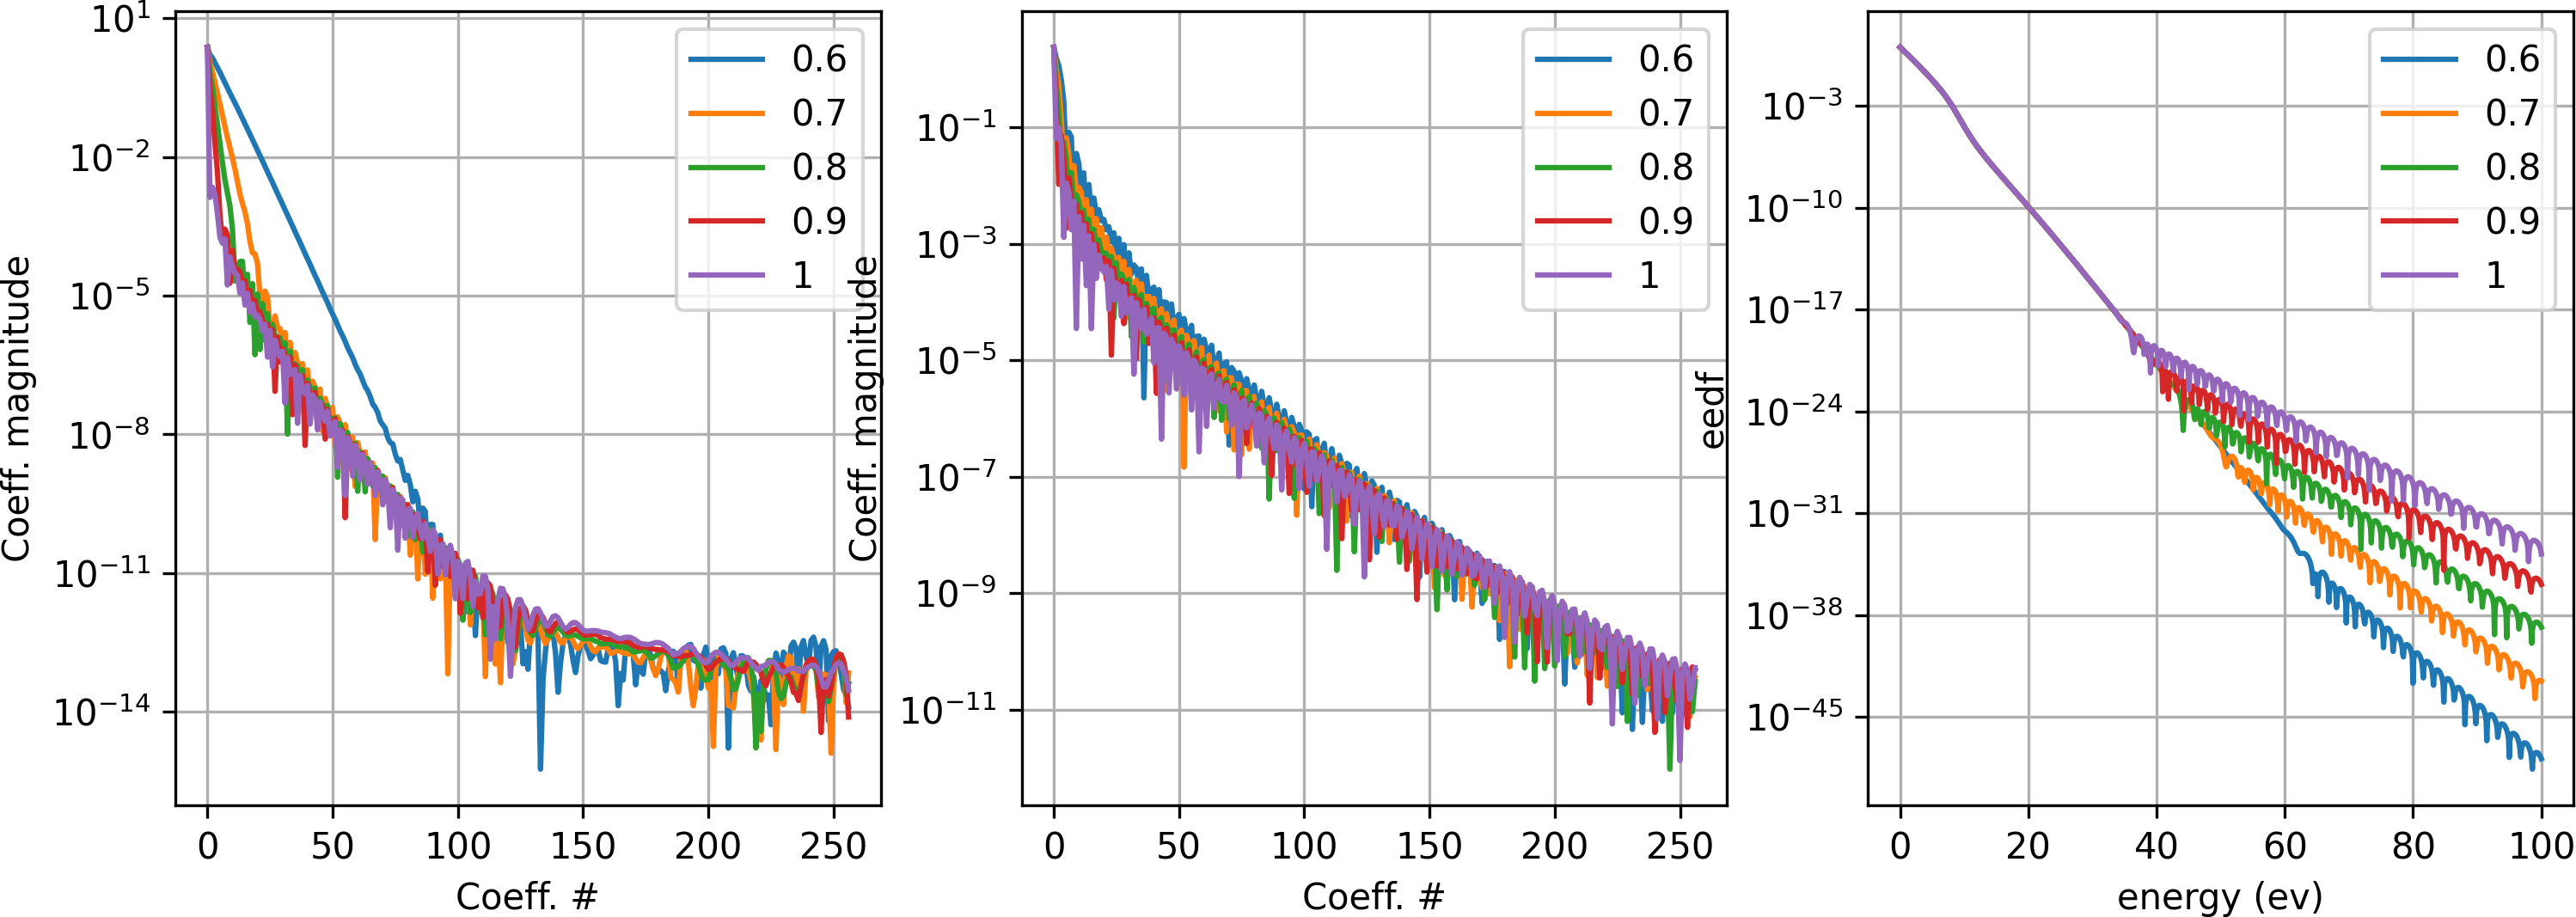
\includegraphics[width=0.99\textwidth]{fig/different_vth_real_1e-6.png}

Constant cross-section $t_{end} = 10^{-5}$ s\\
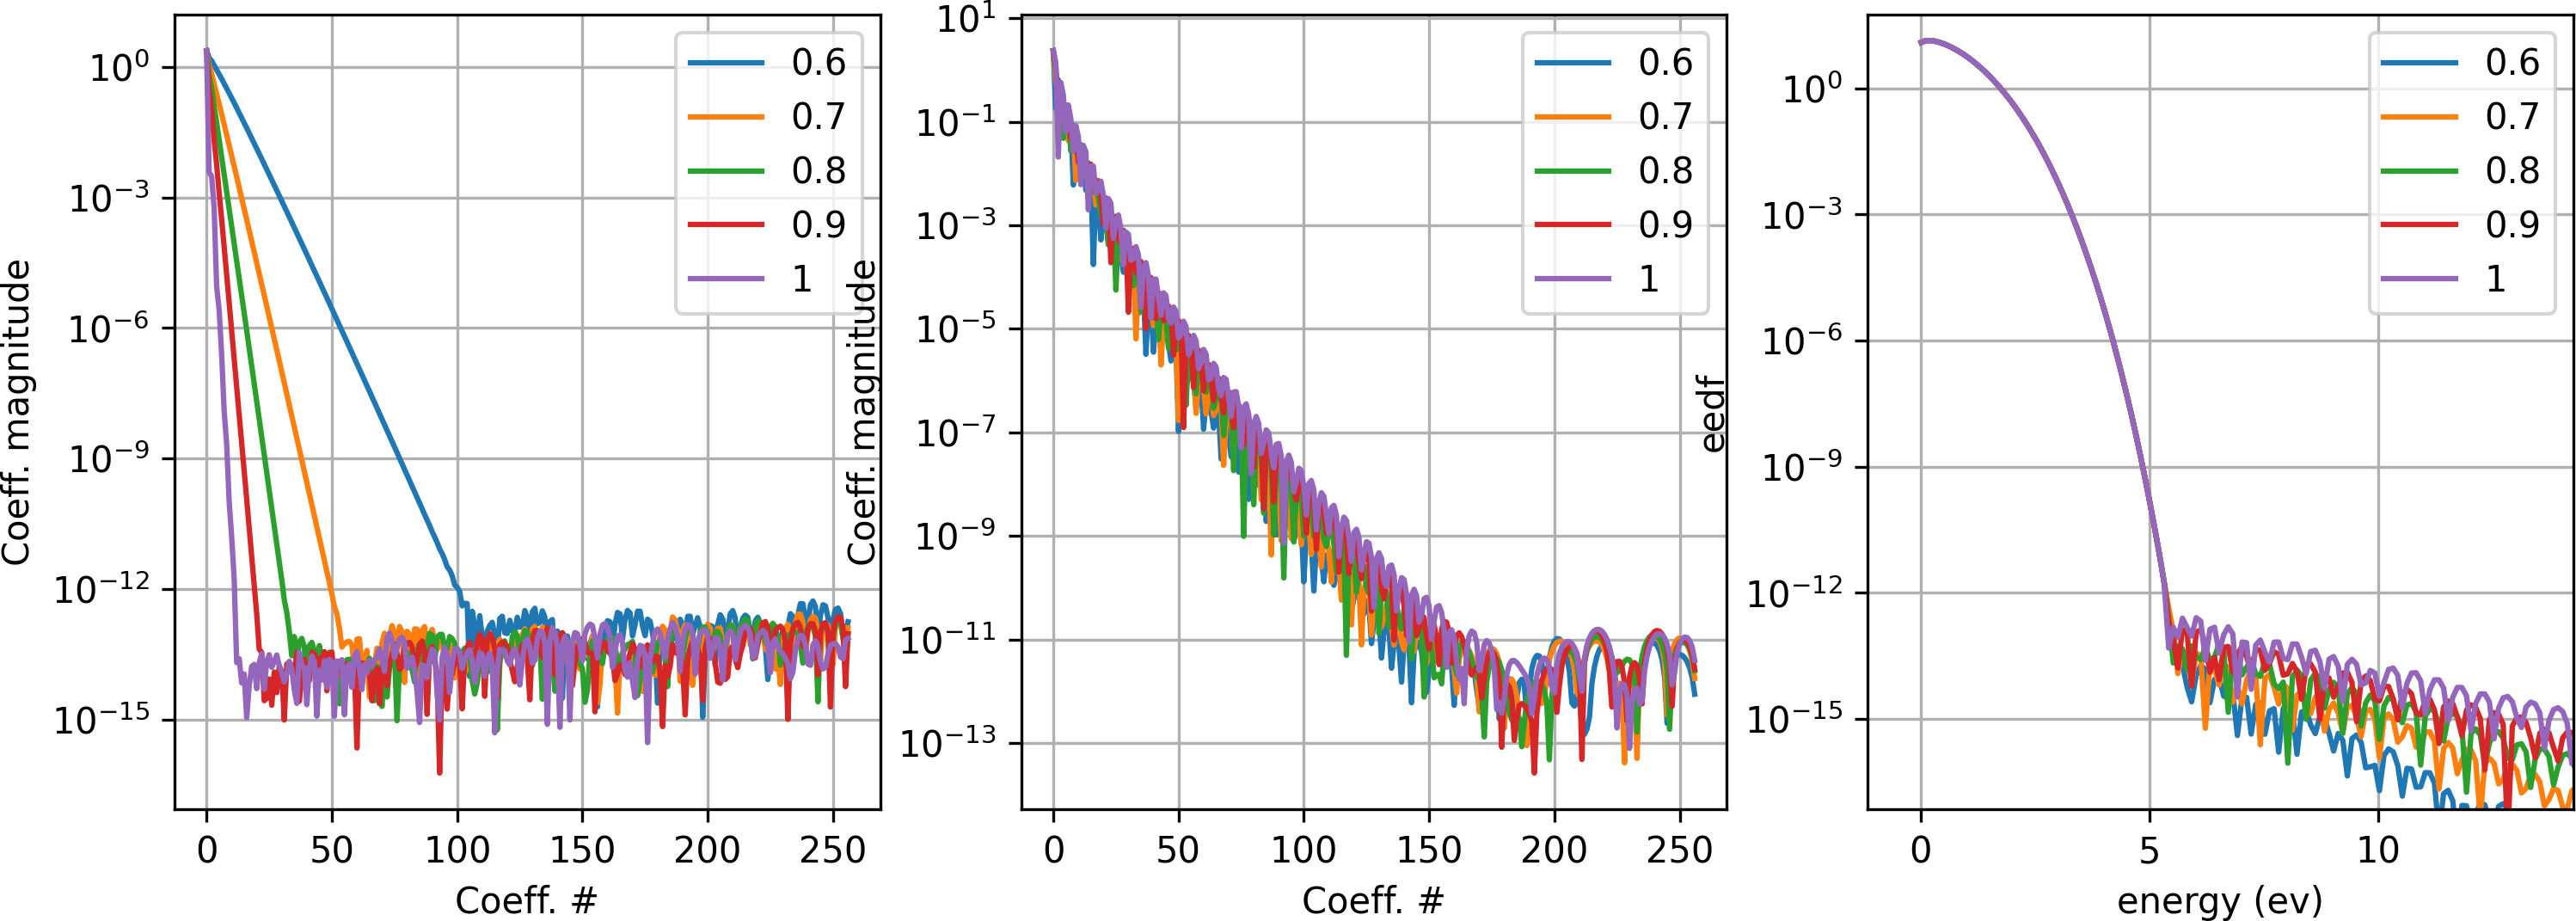
\includegraphics[width=0.99\textwidth]{fig/different_vth_const_1e-5.png}

Data-fitted cross section $t_{end} = 10^{-5}$ s\\
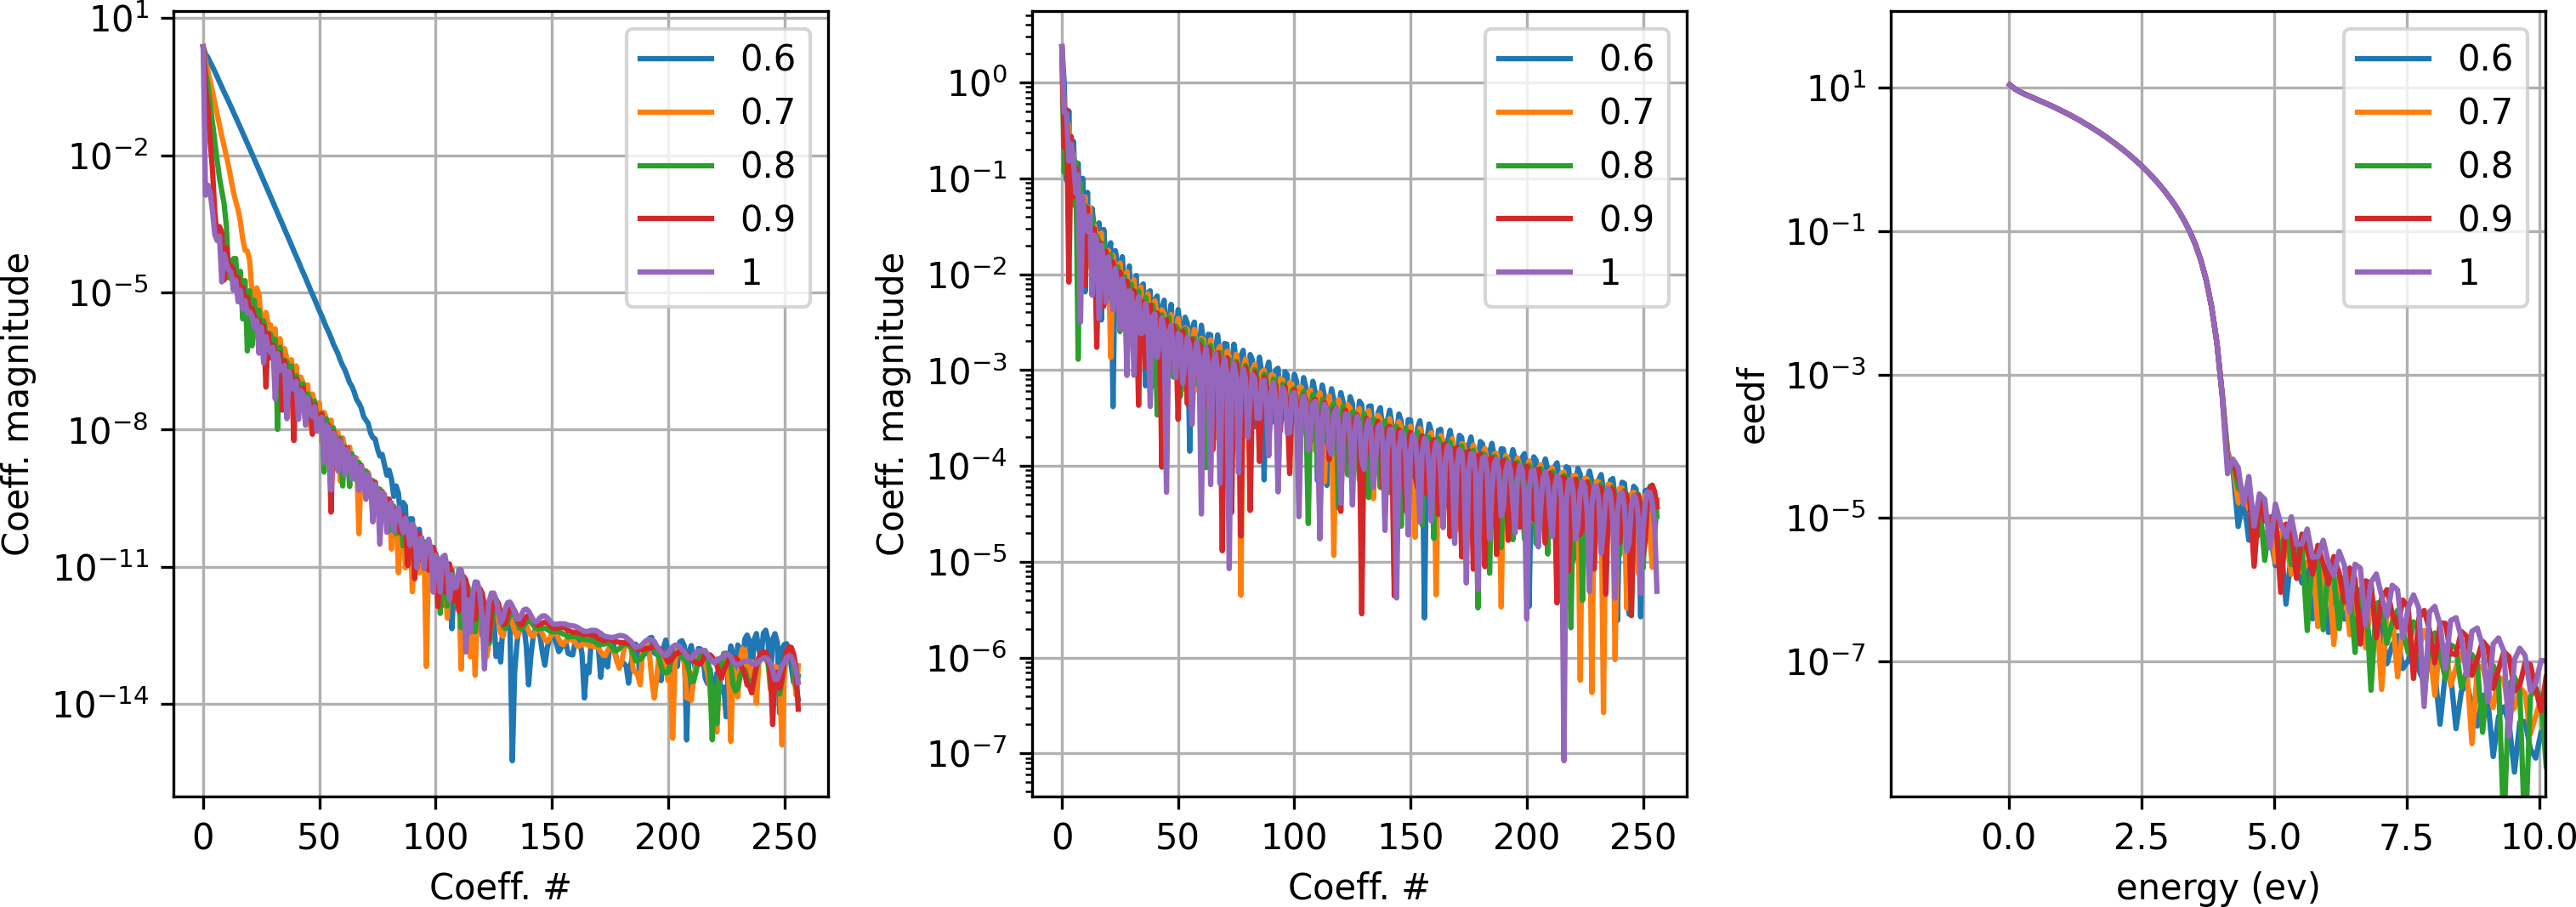
\includegraphics[width=0.99\textwidth]{fig/different_vth_real_1e-5.png}

\newpage
\section{Analytical solutions}

Expansion
%\begin{align*}
%f\of{\vect{v},t} = \sum h_{klm}\of{t} \exp\of{-\frac{v^2}{\vth^2}} \left( \frac{v}{\vth} \right)^{l} P_{kl}\of{\frac{v}{\vth}} Y_{lm}\of{\vtheta, \vphi}
%\end{align*}
\begin{align*}
f\of{\vect{v},t} = \sum h_{klm}\of{t} \Phi_{kl}\of{\vr} Y_{lm}\of{\vtheta, \vphi}
\end{align*}
Total number of electrons
\begin{align*}
n = \myint_{R^3} f\of{\vect{v},t} d\vect{v} = h_{000}\of{t} \myint_{R^3} \Phi_{00}\of{\vr} Y_{00}\of{\vtheta, \vphi} d\vect{v} = \alpha h_{000}\of{t}
\end{align*}
\begin{align*}
Y_{00}\of{\vtheta, \vphi} &= \sqrt{\frac1{4\pi}}
\\
\Phi_{00}\of{\vr} &= \exp\of{ -\left( \frac{v}{\vth} \right)^2 } P_{00} \of{\frac{v}{\vth}}
\end{align*}
\begin{align*}
\alpha = \frac\pi{2} P_{00}\of{0} \vth^3
\end{align*}
System of ODEs for coefficients
\begin{align*}
\frac{d \vect{h}}{dt} + E \vect{h} = C \vect{h}
\end{align*}
Factor out the very first coefficient $h_0\of{t}$:
\begin{align*}
\vect{h} = 
\begin{pmatrix}
h_0 \\ \vect{h}_\ast
\end{pmatrix}
,\quad
E = 
\begin{pmatrix}
0 & \vect{0}^T \\
\vect{e}_{0\ast} & E_{\ast\ast}
\end{pmatrix}
,\quad
C = 
\begin{pmatrix}
C_{00} & \vect{c}_{\ast 0}^T \\
\vect{c}_{0\ast} & C_{\ast\ast}
\end{pmatrix}
\end{align*}
A slightly more explicit systems of ODEs
\begin{align*}
\frac{dh_0}{dt} &= h_0 \left(C_{00} + \vect{c}_{\ast 0}^T \frac{\vect{h}_\ast}{h_0} \right)
\\
\frac{d \vect{h}_\ast}{dt} &= - \vect{e}_{0\ast} h_0 
- E_{\ast\ast} \vect{h}_\ast
- \vect{c}_{0\ast} h_0 
- C_{\ast\ast} \vect{h}_\ast
\end{align*}
Deriving an equation for scaled coefficients $\frac{\vect{h}_\ast}{h_0}$
\begin{align*}
\frac{d}{dt} \left( \frac{\vect{h}_\ast}{h_0} \right) + \frac{\vect{h}_\ast}{h_0^2} \frac{dh_0}{dt} &= 
\left( \vect{c}_{0\ast} - \vect{e}_{0\ast} \right)
+ \left( C_{\ast\ast} - E_{\ast\ast} \right) \frac{\vect{h}_\ast}{h_0}
\end{align*}
Substituting equation for $\frac{dh_0}{dt}$
\begin{align*}
\frac{d}{dt} \left( \frac{\vect{h}_\ast}{h_0} \right) 
+ \frac{\vect{h}_\ast}{h_0} \left(C_{00} + \vect{c}_{\ast 0}^T \frac{\vect{h}_\ast}{h_0} \right) &= 
\left( \vect{c}_{0\ast} - \vect{e}_{0\ast} \right)
+ \left( C_{\ast\ast} - E_{\ast\ast} \right) \frac{\vect{h}_\ast}{h_0}
\end{align*}
\begin{align*}
\frac{d}{dt} \left( \frac{\vect{h}_\ast}{h_0} \right) 
&= 
\left( \vect{c}_{0\ast} - \vect{e}_{0\ast} \right)
+ \left( C_{\ast\ast} - E_{\ast\ast} - \left(C_{00} + \vect{c}_{\ast 0}^T \frac{\vect{h}_\ast}{h_0} \right) I \right) \frac{\vect{h}_\ast}{h_0}
\end{align*}
Steady-state solution
\begin{align*}
\frac{\vect{h}_\ast}{h_0} = 
\left( \left(C_{00} + \vect{c}_{\ast 0}^T \frac{\vect{h}_\ast}{h_0} \right) I
- \left( C_{\ast\ast} - E_{\ast\ast} \right) \right)^{-1}
\left( \vect{c}_{0\ast} - \vect{e}_{0\ast} \right)
\end{align*}


\newpage


System of ODEs for coefficients
\begin{align*}
\frac{d \vect{h}}{dt} + E \vect{h} = C \vect{h}
\end{align*}

Let $\vect{u}$ be some vector, e.g. if $\vect{u} = \begin{pmatrix}
1 & \ldots & 1 
\end{pmatrix}^T$, then $\vect{u}^T \vect{h} = \sum h_i$.
Equation for $\hat{\vect{h}} = \frac{\vect{h}}{\vect{u}^T \vect{h}}$:
\begin{align*}
\frac{d \hat{\vect{h}}}{dt} 
=
\frac{d}{dt} \left( \frac{\vect{h}}{\vect{u}^T \vect{h}} \right) 
&= 
\frac{1}{\vect{u}^T \vect{h}} \frac{d\vect{h}}{dt}
- \frac{\vect{h}}{\vect{u}^T \vect{h}} \frac{\vect{u}^T d\vect{h}/dt}{\vect{u}^T \vect{h}}
\\
&= \left( C - E \right) \hat{\vect{h}} - \hat{\vect{h}} \vect{u}^T \left( C - E \right) \hat{\vect{h}}
\end{align*}

Transient equation for $\hat{\vect{h}}$
\begin{align*}
\frac{d \hat{\vect{h}}}{dt} 
= \left( C - E - \vect{u}^T \left( C - E \right) \hat{\vect{h}} I \right) \hat{\vect{h}}
\end{align*}

Transient equation for $\vect{u}^T \hat{\vect{h}}$
\begin{align*}
\frac{d \vect{u}^T \hat{\vect{h}}}{dt} 
= \left( 1 - \vect{u}^T \hat{\vect{h}} \right) \vect{u}^T \left( C - E \right) \hat{\vect{h}}
\end{align*}
Note that, if $\vect{u}^T \hat{\vect{h}} = 1$ at the initial time instant $t=0$, then $\frac{d \vect{u}^T \hat{\vect{h}}}{dt} = 0$ and $\vect{u}^T \hat{\vect{h}} = 1$ for any $t>0$. \textbf{Question:} if $\vect{u}^T \hat{\vect{h}} = 1+\varepsilon$ due to machine precision, would it lead to instability?


At the steady-state one should have $\frac{d \hat{\vect{h}}}{dt} = 0$ subject to $\vect{u}^T \hat{\vect{h}} = 1$ (by construction). 

\newpage

\begin{align*}
n_e(t) &= \int_{\vect{v}} f(t, \vect{v}) \diff{\vect{v}} \text{ and } a(t) = \frac{1}{n_e(t)}
\end{align*}
The normalized distribution function $\hat{f}(t,\vect{v}) = a(t) f(t, \vect{v})$. Write the Boltzmann equation in the normalized $\hat{f}(t, \vect{v})$. For distribution function $f$, we can write, 
\begin{align*}
	\partial_t f\of{t,\vect{v}} &= (C-E)f \\
	\partial_t\of{a\of{t} f\of{t,\vect{v}}} &= \dot{a}\of{t}f\of{t,\vect{v}} + a\of{t} \dot{f}\of{t,\vect{v}} \\
											&= \dot{a}\of{t}f + a\of{t} (C-E)f \\
											&= -\dot{n}_e\of{t} a^2\of{t} f + a\of{t} (C-E)f \\
\end{align*}
we can re-write the above with the normalized distribution $\hat{f}$, 
\begin{align*}
\partial_t\of{\hat{f}(t,\vect{v})} &=-\dot{n}_e\of{t} a\of{t} \hat{f} + (C-E)\hat{f}
\end{align*}. In the continuous form, 
\begin{align*}
\dot{n}_e (t) = \int_\vect{v} \dot{f} \diff{\vect{v}} &= \int_\vect{v} C(f) \diff{v} - \int_\vect{v} \vect{E} \cdot \nabla_\vect{v} f \diff{\vect{v}} \\
&= \int_\vect{v} C(f) \diff{v} -\int_\vect{v} \nabla_\vect{v} \cdot (\vect{E} f) \diff{\vect{v}} \\
&= \int_\vect{v} C(f) \diff{v} -\int_{\partial\vect{v}} (\vect{E} f) \cdot \vect{n} \diff\vect{s}
\end{align*}


where, 
\begin{align*}
\dot{n}_e (t) = \int \dot{f} dv &= \int (C-E) f dv = \int C f dv \\
\frac{\dot{n}_e (t)}{n_e(t)} &=\int C \hat{f} dv \\
\partial_t\of{\hat{f}(t,\vect{v})} &=-\left(\int C \hat{f} dv \right) \hat{f} + (C-E)\hat{f}
\end{align*}
For the steady state, we can write, 
\begin{align*}
	\partial_t\of{\hat{f}} &=0 \implies -\left(\int C \hat{f} dv \right) \hat{f} + (C-E)\hat{f} =0 \\ 
\end{align*}
let $u^T f$ be the mass of the distribution function, by construction, $u^T \hat{f}=1$.
\begin{align*}
 -(u^T C \hat{f}) \hat{f} + (C-E)\hat{f} =0 \\ 
\end{align*} 
Let, 
\begin{align*}
R(f)&=
\begin{pmatrix}
-(u^T C f) f + (C-E)f \\
u^Tf-1
\end{pmatrix}
\end{align*} For the steady  state we need $R(f) = \vect{0}$. The Jacobian for the $R$ is given by, 
\begin{align*}
J(f)&=
\begin{pmatrix}
-2(u^T C f) I + (C-E) \\
u^T
\end{pmatrix}
\end{align*}




%\begin{align*}
%\partial_t\of{a\of{t} f\of{t,\vect{v}}} + \vect{E} \cdot \nabla_\vect{v}\of{a\of{t} f\of{t,\vect{v}}}  & = C\of{a(t) f(t, \vect{v})} \\
%\dot{a}\of{t}f\of{t,\vect{v}} + a\of{t} \dot{f}\of{t,\vect{v}} +  a\of{t} \vect{E} \cdot \nabla_\vect{v}\of{f\of{t,\vect{v}}} &= C\of{a(t) f(t, \vect{v})}\\
%\end{align*}



%Attempt to compute the steady state solution analytically for B-splines. 
%\begin{align*}
%f\of{\vect{v},t} = \sum h_{klm}\of{t} \Phi_{kl}\of{\vr} Y_{lm}\of{\vtheta, \vphi}
%\end{align*}
%Total number of electrons
%\begin{align*}
%n = \myint_{R^3} f\of{\vect{v},t} d\vect{v} = \sum_{k} h_{k00}\of{t} \myint_{R^3} \Phi_{k0}\of{\vr} Y_{00}\of{\vtheta, \vphi} d\vect{v} = W_{p00}^T h_{p00}
%\end{align*} where $W_{p00} = \myint_{R^3} \Phi_{k0}\of{\vr} Y_{00}\of{\vtheta, \vphi} d\vect{v} $.
%
%\begin{align*}
%\vect{h} = 
%\begin{pmatrix}
%h_{k00} \\ \vect{h}_\ast
%\end{pmatrix}
%,\quad
%E = 
%\begin{pmatrix}
%0 & \vect{0}^T \\
%\vect{e}_{0\ast} & E_{\ast\ast}
%\end{pmatrix}
%,\quad
%C = 
%\begin{pmatrix}
%C_{00} & \vect{c}_{\ast 0}^T \\
%\vect{c}_{0\ast} & C_{\ast\ast}
%\end{pmatrix}
%\end{align*}



\newpage

\begin{align*}
\vect{h} =
\begin{pmatrix}
h_0 \\
\tilde{\vect{h}}
\end{pmatrix}
,\quad
C = 
\begin{pmatrix}
0 & \vect{0}^T \\
\vect{c}_0 & \tilde{C}
\end{pmatrix}
\end{align*}
\begin{align*}
\frac{d \tilde{\vect{h}}}{dt} = \tilde{C} \tilde{\vect{h}} + h_0 \vect{c}_0
\end{align*}

\begin{align*}
\tilde{C} &= V \Lambda V^{-1}
\end{align*}

\begin{align*}
\tilde{\vect{h}}\of{t} = V \exp\of{\Lambda t} V^{-1} \tilde{\vect{h}}\of{0} + h_0 V \left( I - \exp\of{\Lambda t} \right) \Lambda^{-1} V^{-1} \vect{c}_0
\end{align*}

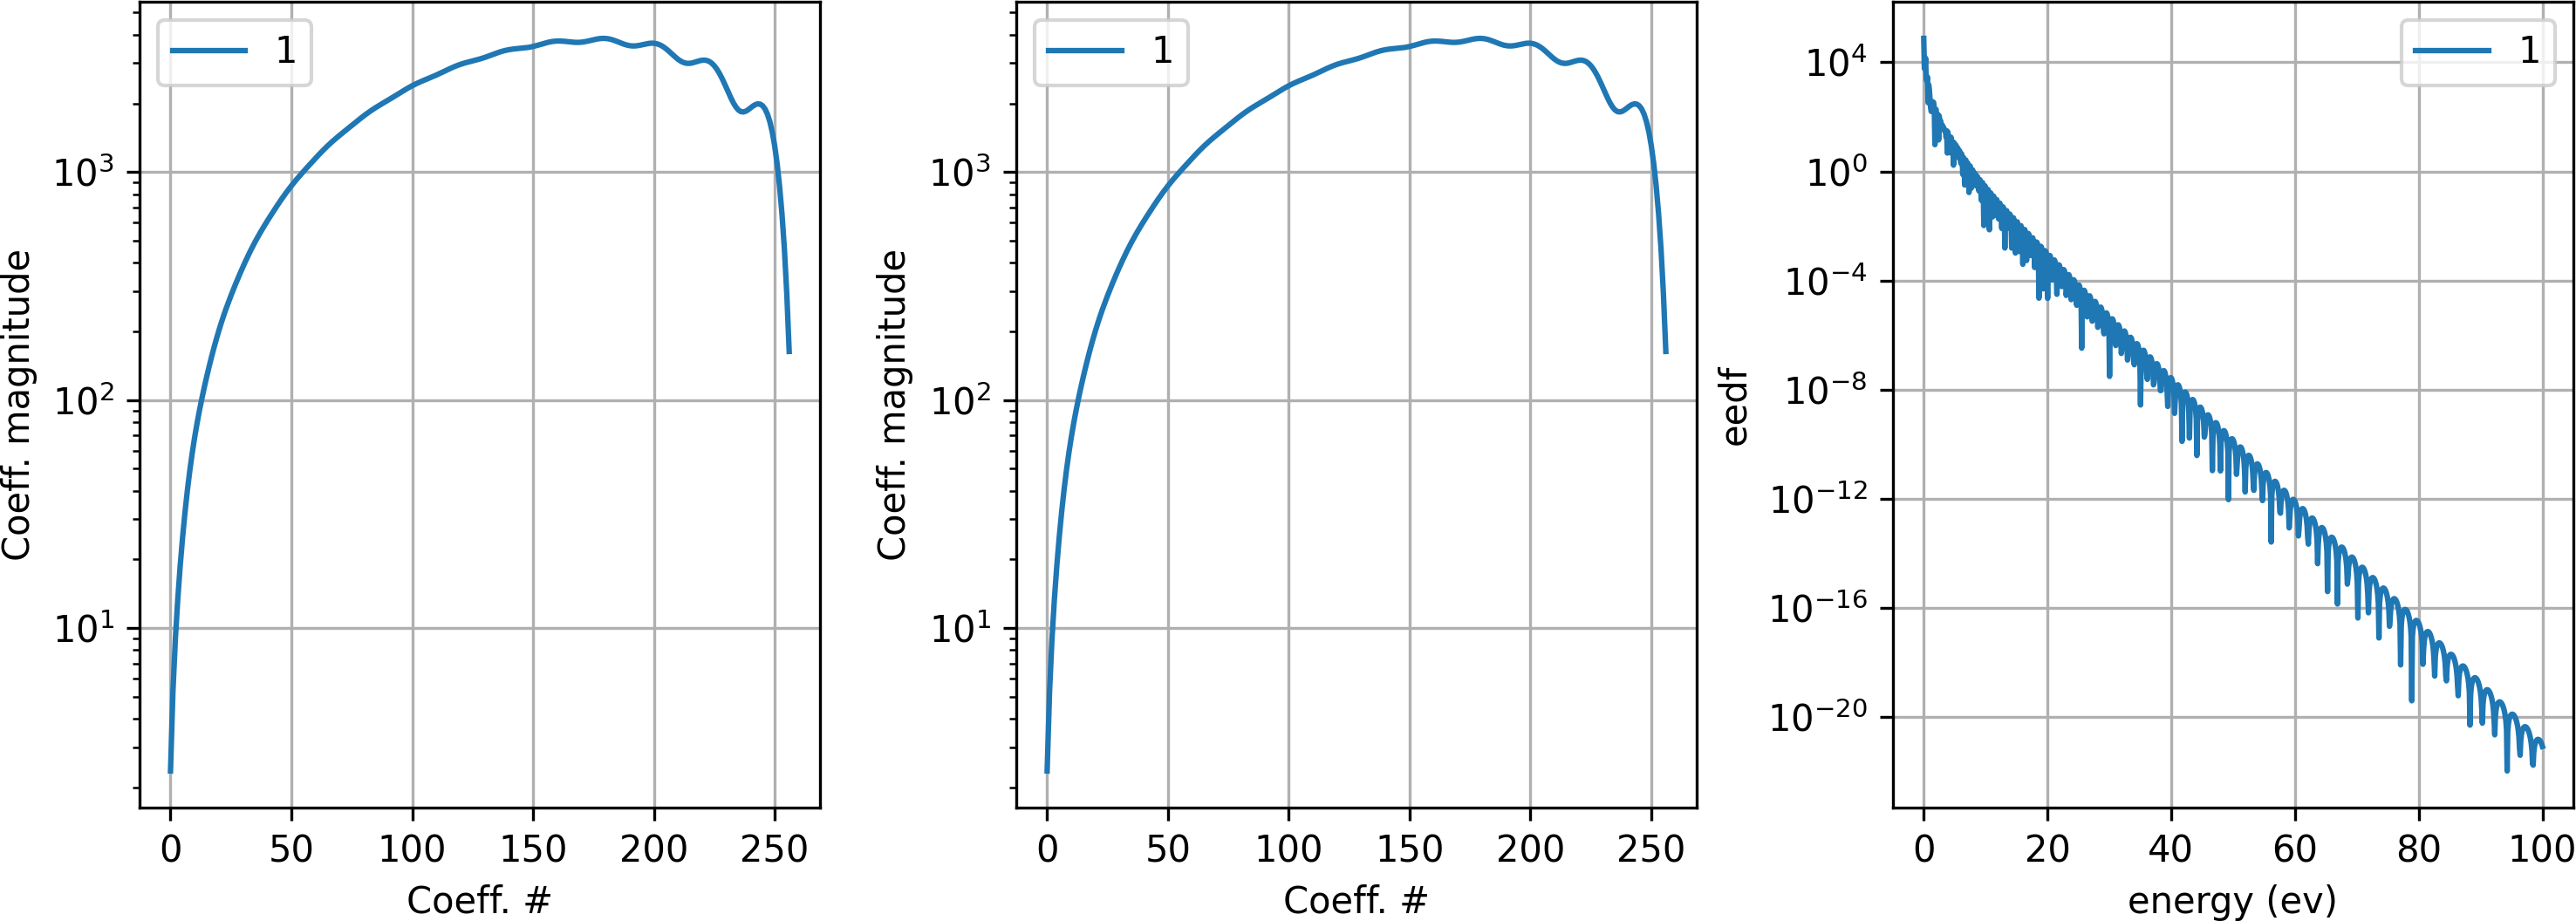
\includegraphics[width=0.99\textwidth]{fig/steady_state_elastic_only.png}

\newpage
System of ODEs for coefficients
\begin{align*}
\frac{d \vect{h}}{dt} - E \sin\of{\omega t} \vect{h} = C \vect{h}
\end{align*}
Eigenvalue decomposition of $C$:
\begin{align*}
C &= V \Lambda V^{-1}
\end{align*}
Change of variables:
\begin{align*}
\vect{y} &= V^{-1} \vect{h} \\
F &= V^{-1} E V
\end{align*}
New form:
\begin{align*}
\frac{d \vect{y}}{dt} - F \sin\of{\omega t} \vect{y} = \Lambda \vect{y}
\end{align*}
A Floquet-Lyapunov transformation:
\begin{align*}
\vect{y} = \exp\of{-\frac{F}{\omega} \cos{\omega t} + \Lambda t} \vect{z}
\end{align*}
leads to:
\begin{align*}
\frac{d \vect{z}}{dt} = 0
\end{align*}
thus:
\begin{align*}
\vect{h}\of{t} = V \exp\of{\frac{V^{-1} E V}{\omega}  \left(1 - \cos\of{\omega t} \right) + \Lambda t} V^{-1} \vect{h}\of{0}
\end{align*}

\newpage
\begin{align*}
\vect{h} =
\begin{pmatrix}
h_0 \\
\tilde{\vect{h}}
\end{pmatrix}
,\quad
C = 
\begin{pmatrix}
0 & \vect{0}^T \\
\vect{c}_0 & \tilde{C}
\end{pmatrix}
\end{align*}
\begin{align*}
\frac{d \tilde{\vect{h}}}{dt} - E \sin\of{\omega t} \tilde{\vect{h}} = \tilde{C} \tilde{\vect{h}} + h_0 \vect{c}_0
\end{align*}
Change of variables:
\begin{align*}
\vect{y} &= \tilde{V}^{-1} \tilde{\vect{h}} \\
F &= \tilde{V}^{-1} \tilde{E} \tilde{V}\\
\vect{g} &= \tilde{V}^{-1} h_0 \vect{c}_0
\end{align*}
New form:
\begin{align*}
\frac{d \vect{y}}{dt} - F \sin\of{\omega t} \vect{y} = \Lambda \vect{y} + \vect{g}
\end{align*}
After a Floquet-Lyapunov transformation:
\begin{align*}
\exp\of{-\frac{F}{\omega} \cos{\omega t} + \Lambda t} \frac{d \vect{z}}{dt} = \vect{g}
\end{align*}
Solving:
\begin{align*}
\vect{z}\of{t} = \vect{z}\of{0} + \int_{0}^{t} \exp\of{\frac{F}{\omega} \cos{\omega \tau} - \Lambda \tau} d\tau \vect{g} 
\end{align*}

\begin{multline*}
\tilde{\vect{h}}\of{t} = \tilde{V} \exp\of{\frac{\tilde{V}^{-1} \tilde{E} \tilde{V}}{\omega} \left(1 - \cos\of{\omega t}\right) + \Lambda t} V^{-1} \tilde{\vect{h}}\of{0}
\\
+
h_0
\tilde{V} 
\int_{0}^{t} \exp\of{\frac{\tilde{V}^{-1} \tilde{E} \tilde{V}}{\omega} \left( \cos\of{\omega \tau} - \cos\of{\omega t} \right)  - \Lambda \left( \tau - t \right)} d\tau V^{-1} \vect{c}_0
\end{multline*}


\end{document}
